%-----------------------------------------------------------------------------%
% Set metadata for use with pdfx
%\begingroup\newif\ifmy
%\IfFileExists{\jobname.xmpdata}{}{\mytrue}
%\ifmy
%\begin{filecontents*}{\jobname.xmpdata}
%\Title{Data Science Notes}
%\Author{Matthew Epland, Ph.D.}
%\Keywords{Data Science\sep Machine Learning\sep Statistics}
%\Copyright{CC-BY-4.0}
%\end{filecontents*}
%\fi\endgroup

% \Subject{TODO}

%-----------------------------------------------------------------------------%
% Set documentclass
\documentclass[nogradschool,singlespace,nobind]{dukedissertation_modified}

%-----------------------------------------------------------------------------%
% usepackages
\usepackage{amsmath,amssymb,bbm,bm} % https://ctan.org/pkg/bm
\usepackage{mathtools}
\usepackage{cancel}
\usepackage{graphicx}
\usepackage{xcolor}
\usepackage{textcomp} % needed to fix \mico \textmu from siunitx to work with microtype: https://tex.stackexchange.com/questions/74670/microtype-siunitx-and-micro-mysterious-warnings
\usepackage[protrusion=true,expansion=true]{microtype} % make text flow nicely... might screw up duke dissertation template
\usepackage{verbatim} % verbatim text and comment environment
\usepackage{lmodern} % allowing font sizes at arbitrary sizes
\usepackage{notoccite} % fixes citation numbering in captions with respect to lof & lot, see https://ctan.org/pkg/notoccite
\usepackage[nocompress]{cite} % orders references numerically within one \cite{}, see https://tex.stackexchange.com/questions/69230/numbered-ordering-of-multiple-citations Also changes spacing after comma
\usepackage{fnpct} % make multiple footnotes at one point look nice, https://tex.stackexchange.com/questions/28465/multiple-footnotes-at-one-point
\usepackage[separate-uncertainty,multi-part-units=single,free-standing-units,product-units=repeat,use-xspace,binary-units]{siunitx} % units package, see https://www.ctan.org/pkg/siunitx
\sisetup{range-phrase={\text{--}},range-units=single}
\usepackage{physics}
\usepackage{booktabs,array,multirow,diagbox}
\renewcommand{\arraystretch}{1.5} % gives extra height to tabular rows for super/subscripts
%\usepackage{longtable}
\usepackage{enumitem}
\usepackage{lscape} % landscape https://ctan.org/pkg/lscape
\usepackage{moresize}
\usepackage{listings}
\usepackage[T1]{fontenc}

\usepackage[top=1in, bottom=1.25in, left=1.25in, right=1.25in]{geometry}
\usepackage{fancyhdr}
\pagestyle{plain}

% use subcaption to get split figures, but the caption dependency doesn't know about the dukedissertation document class - turn off the warning with silence
% load caption explicitly first to set it's options, subcaption says it passes them through but it doesn't seem to work
% https://tex.stackexchange.com/questions/34579/is-there-really-something-wrong-with-using-the-caption-package-for-continuedflo
% https://en.wikibooks.org/wiki/LaTeX/Floats,_Figures_and_Captions#Subfloats
% https://ctan.org/pkg/caption
% https://ctan.org/pkg/subcaption
\usepackage{silence}
\WarningFilter{caption}{Unsupported document class}
\WarningFilter{hyperref}{The PDF version number could not be set}
\usepackage{setspace} % needed to specify, https://ctan.org/pkg/setspace
\usepackage[style=base,skip=2pt,width=\textwidth]{caption} % ,font={stretch=1.3}
\usepackage[skip=1pt]{subcaption}
\newsavebox{\largestimage} % see https://tex.stackexchange.com/questions/239128/subcaption-vertical-alignment-of-two-images-of-different-vertical-size

% Don't let floats get before the subsection where they're included
% https://tex.stackexchange.com/questions/32598/force-latex-image-to-appear-in-the-section-in-which-its-declared
% https://tex.stackexchange.com/questions/279/how-do-i-ensure-that-figures-appear-in-the-section-theyre-associated-with/235312#235312
% Also doesn't let a float go into a following subsection, results in a ton of blank space - probably better left off
% \usepackage{placeins}
%\let\Oldsubsection\subsection
%\renewcommand{\subsection}{\FloatBarrier\Oldsubsection}

\usepackage{float} % to allow for H option. Works better than \FloatBarrier from placeins, though it is more manual
\floatstyle{plaintop}
\restylefloat{table}

% keep footnotes from splitting, can still happen sometimes (10000 forces)
% https://tex.stackexchange.com/questions/32208/footnote-runs-onto-second-page
\interfootnotelinepenalty=9999

% keep inline equations from splitting, can still happen sometimes (10000 forces)
% https://tex.stackexchange.com/a/14243
\relpenalty=9999
\binoppenalty=9999

%-----------------------------------------------------------------------------%
% Other possibly useful packages
% \usepackage{fancyvrb}
% \usepackage{ulem}
% \usepackage{overpic}
% \usepackage{amsfonts, amsthm}
% \usepackage{mathabx}

%-----------------------------------------------------------------------------%
% tweak listings
\definecolor{codegreen}{rgb}{0,0.6,0}
\definecolor{codegray}{rgb}{0.5,0.5,0.5}
\definecolor{codemauve}{rgb}{0.58,0,0.82}

\lstset{
  backgroundcolor=\color{white},     % choose the background color; you must add \usepackage{color} or \usepackage{xcolor}; should come as last argument
  % basicstyle=\ssmall,                % the size of the fonts that are used for the code
  basicstyle=\ttfamily,              % make font tt
  upquote=true,                      % make all single quotes straight up and down
  breakatwhitespace=false,           % sets if automatic breaks should only happen at whitespace
  breaklines=true,                   % sets automatic line breaking
  captionpos=b,                      % sets the caption-position to bottom
  commentstyle=\color{codegreen},    % comment style
  % deletekeywords={...},            % if you want to delete keywords from the given language
  % escapeinside={\%*}{*)},          % if you want to add LaTeX within your code
  extendedchars=true,                % lets you use non-ASCII characters; for 8-bits encodings only, does not work with UTF-8
  firstnumber=1,                     % start line enumeration with line 1000
  frame=none,                        % adds a frame around the code
  keepspaces=true,                   % keeps spaces in text, useful for keeping indentation of code (possibly needs columns=flexible)
  keywordstyle=\color{blue},         % keyword style
  % language=Octave,                 % the language of the code
  % morekeywords={*,...},            % if you want to add more keywords to the set
  numbers=left,                      % where to put the line-numbers; possible values are (none, left, right)
  numbersep=5pt,                     % how far the line-numbers are from the code
  numberstyle=\ttfamily\tiny\color{codegray}, % the style that is used for the line-numbers
  rulecolor=\color{black},           % if not set, the frame-color may be changed on line-breaks within not-black text (e.g. comments (green here))
  showspaces=false,                  % show spaces everywhere adding particular underscores; it overrides 'showstringspaces'
  showstringspaces=false,            % underline spaces within strings only
  showtabs=false,                    % show tabs within strings adding particular underscores
  stepnumber=1,                      % the step between two line-numbers. If it's 1, each line will be numbered
  stringstyle=\color{codemauve},     % string literal style
  tabsize=2,                         % sets default tabsize to 2 spaces
}

%-----------------------------------------------------------------------------%
% Include abbreviations
\usepackage{xspace}
 % note that \xspace properly handles the abbreviation period spacing - producing a single regular space, not the end of a sentence spacing

% https://tex.stackexchange.com/questions/7032/good-way-to-make-textcircled-numbers
% \usepackage{tikz}
% \DeclareRobustCommand{\circled}[1]{\tikz[baseline=(char.base)]{\node[shape=circle,draw,inner sep=1pt] (char) {#1};}}

% general, https://tex.stackexchange.com/questions/2229/is-a-period-after-an-abbreviation-the-same-as-an-end-of-sentence-period/2230#2230
\newcommand*{\ie}{\textit{i.e.}\@\xspace}
\newcommand*{\eg}{\textit{e.g.}\@\xspace}
%\newcommand*{\etc}{\textit{etc.}\@\xspace}
\makeatletter
\newcommand\etc{\textit{etc}\@ifnextchar.{}{.\@\xspace}}
\makeatother

% \newcommand{\orderof}{\ensuremath{\mathcal{O}}} % use \order from physics package instead
\newcommand{\lagr}{\ensuremath{\mathcal{L}}\xspace}
\newcommand{\transpose}{\ensuremath{^{\text{T}}}\xspace}
\newcommand{\stcomp}[1]{\overline{#1}}
\newcommand{\identity}{\ensuremath{I}\xspace} % note \mathbb{1} did not work
% \newcommand{\dif}{\mathop{}\!\mathrm{d}} % I think dt looks just fine
% \newcommand{\dif}{d} % I think dt looks just fine
\newcommand*{\dif}{\ensuremath{d}} % from ATLAS def

\DeclareMathOperator*{\sign}{sgn}

\DeclareMathOperator*{\argmin}{arg\,min} % thin space, limits underneath in displays, https://tex.stackexchange.com/questions/5223/command-for-argmin-or-argmax
\DeclareMathOperator*{\argmax}{arg\,max}

\newcommand*{\cov}[2]{\ensuremath{\text{cov}\left(#1,#2\right)}\xspace}
\newcommand*{\variance}[1]{\ensuremath{\text{var}\left(#1\right)}\xspace}
\newcommand*{\bias}[1]{\ensuremath{\text{bias}\left(#1\right)}\xspace}

\newcommand*{\expvalE}[1]{\ensuremath{E\left(#1\right)}\xspace}

\newcommand*{\pvalue}{\ensuremath{p\text{-value}}\xspace}

\newcommand*{\insitu}{\text{\textit{in~situ}}\xspace}
\newcommand*{\Insitu}{\text{\textit{In~situ}}\xspace}
\newcommand*{\InSitu}{\text{\textit{In~Situ}}\xspace}

\newcommand*{\apriori}{\text{\textit{a~priori}}\xspace}
\newcommand*{\aposteriori}{\text{\textit{a~posteriori}}\xspace}

\newcommand*{\CLs}{\ensuremath{CL_{s}}\xspace}

\newcommand*{\yhatBDT}{\ensuremath{\hat{y}_{\text{BDT}}}\xspace}
\newcommand*{\yhat}{\ensuremath{\hat{y}}\xspace}

% Software packages
\newcommand*{\xgboost}{\textsc{XGBoost}\xspace}
\newcommand*{\uprootPackage}{\textsc{uproot}\xspace} % \uproot already exists
\newcommand*{\python}{\textsc{Python}\xspace}
\newcommand*{\R}{\textsc{R}\xspace}
\newcommand*{\sql}{\textsc{SQL}\xspace}
\newcommand*{\pandas}{\textsc{Pandas}\xspace}
\newcommand*{\pyspark}{\textsc{PySpark}\xspace}
\newcommand*{\numpy}{\textsc{NumPy}\xspace}
\newcommand*{\scipy}{\textsc{SciPy}\xspace}
\newcommand*{\sklearn}{\textsc{Scikit-Learn}\xspace}
\newcommand*{\skopt}{\textsc{Scikit-Optimize}\xspace}
\newcommand*{\networkx}{\textsc{NetworkX}\xspace}
\newcommand*{\ROOT}{\textsc{ROOT}\xspace}
\newcommand*{\TMVA}{\textsc{TMVA}\xspace}
\newcommand*{\HF}{\textsc{HistFitter}\xspace}
\newcommand*{\hfactory}{\textsc{HistFactory}\xspace}
\newcommand*{\roostats}{\textsc{RooStats}\xspace}
\newcommand*{\roofit}{\textsc{RooFit}\xspace}


%-----------------------------------------------------------------------------%
% Include tikz figures which can not be made standalone, only if they have internal references / citations. Also must be manually added to Makefile if they use feynmp

%-----------------------------------------------------------------------------%
% Theorem, Lemma, etc. environments
%\newtheorem{theorem}{Theorem}%[section]
%\newtheorem{lemma}[theorem]{Lemma}
%\newtheorem{proposition}[theorem]{Proposition}
%\newtheorem{corollary}[theorem]{Corollary}
%\newtheorem{result}[theorem]{Result}

%-----------------------------------------------------------------------------%
% PREAMBLE
%-----------------------------------------------------------------------------%
\author{Matthew Epland, Ph.D.}
\title{Data Science Notes}
\date{\today}
%-----------------------------------------------------------------------------%

%-----------------------------------------------------------------------------%
% HYPERREF
%-----------------------------------------------------------------------------%
\usepackage[hyperpageref]{backref} % pages

% need to load in this order to get proper pdfx a-2b format!!!
\PassOptionsToPackage{hyperfootnotes,pagebackref}{hyperref}

% comment out \usepackage{hyperref} and \hypersetup if using pdfx
\usepackage{hyperref}
\makeatletter\hypersetup{
    breaklinks, baseurl=http://, pdfborder=0 0 0, pdfpagemode=UseNone, pdfstartpage=1, bookmarksopen=false, bookmarksdepth=2, % to show sections and subsections
    pdfauthor      = {Matthew Epland, Ph.D.}, %
    pdftitle       = {Data Science Notes}, %
    pdfsubject     = {Data Science, Machine Learning, Statistics}, %
    pdfkeywords    = {Data Science, Machine Learning, Statistics}
}\makeatother

% \usepackage[a-2b]{pdfx} % Note pdfx does not work with travis CI due to latest ubuntu image being from 2016, thus containing this bug https://bugs.debian.org/cgi-bin/bugreport.cgi?bug=877167 fixed in oct 2017. Can use locally if desired

\hypersetup{plainpages=false, bookmarksnumbered,
            % draft, % for printing
            colorlinks, linkcolor=blue, citecolor=blue, urlcolor=blue, % for web
            % breaklinks=true,
           }

% adapted from https://tex.stackexchange.com/questions/183702/formatting-back-references-in-bibliography-bibtex
\renewcommand*{\backrefalt}[4]{%
%    \ifcase #1 Not cited.%
    \ifcase #1% Not cited.%
          \or Cited on page~#2.%
          \else Cited on pages #2.%
    \fi%
    }

%-----------------------------------------------------------------------------%
% use cref and not ref, have to load last
\usepackage[capitalise]{cleveref} % https://ctan.org/pkg/cleveref see section 7.1, if redefining need to make them caps
\crefname{figure}{Figure}{Figures}
\Crefname{figure}{Figure}{Figures}
\crefname{tabular}{Table}{Tables}
\Crefname{tabular}{Table}{Tables}
\crefname{section}{Section}{Sections}
\Crefname{section}{Section}{Sections}
\crefname{chapter}{Chapter}{Chapters}
\Crefname{chapter}{Chapter}{Chapters}
\crefname{appchap}{Appendix}{Appendices}
\Crefname{appchap}{Appendix}{Appendices}
\crefformat{equation}{(#2#1#3)}

\newcommand\preface{%
   \nmchapter{Preface}
}

\begin{document}

%-----------------------------------------------------------------------------%
% TITLE PAGE
%-----------------------------------------------------------------------------%
\maketitle

%-----------------------------------------------------------------------------%
% ABSTRACT -- included file should start with '\abstract'.
%-----------------------------------------------------------------------------%
% \include{{sections/abstract}}

%-----------------------------------------------------------------------------%
% FRONTMATTER
%-----------------------------------------------------------------------------%
\tableofcontents % Automatically generated
\backrefsetup{disable}
\abbreviations

\section*{Symbols}

\begin{symbollist}
  \item[$P\left(X \mid Y\right)$] (Conditional) Probability of $X$ Given $Y$
  \item[$\expval{X}$ or $\expvalE{X}$] Expectation Value of $X$
  \item[$\sigma_{X}^{2}$ or $\variance{X}$] Variance of $X$
  \item[$\sigma_{u,v}^{2}$ or $\cov{u}{v}$] Covariance of $u$ and $v$
  \item[$\bm{\beta}$] Model Parameters, $n \times 1$ Column Vector
  \item[$\mathbf{X}$] Input Features, $m \times n$ Matrix
  \item[$y$] Dependent Feature
  \item[$m$] Number of Data Points or Rows% TODO sometimes n
  \item[$n$] Number of Input Features or Columns
  \item[$\nu$] Number of Degrees of Freedom
  \item[$S\left(\bm{\beta}\right)$] Objective Function
  \item[$L\left(\bm{\beta}\right)$] Loss Function
  \item[$\Omega\left(\bm{\beta}\right)$] Regularization Function
  \item[$L$] Likelihood Function
  \item[$\yhat$] Estimated Dependent Feature or Classification Score, Prediction
  \item[$Z$] Significance
  \item[$S\left(t\right)$] Survival Function
  \item[$\lambda\left(t\right)$] Hazard Function
  % \item[\ZB] Significance, Incomplete Beta Function Approximation
  % \item[\CLs] Signal Confidence Level
\end{symbollist}

\clearpage
\section*{Abbreviations}
% TODo keep updated

\begin{symbollist}
  \item[$k$-NN] $k$-Nearest Neighbors
  \item[ABC] Approximate Bayesian Computation
  \item[ACF] Auto-Correlation Function
  \item[ADF] Augmented Dickey--Fuller Test for Stationarity
  \item[AIC] Akaike Information Criterion
  \item[ANCOVA] Analysis of Covariance
  \item[ANOVA] Analysis of Variance
  \item[AR] Autoregressive (Models)
  \item[AUC] Area Under Curve
  \item[BDT] Boosted Decision Tree
  \item[BIC] Bayesian Information Criterion
  \item[BLUE] Best Linear Unbiased Estimator
  \item[CART] Classification and Regression Tree
  \item[CDF] Cumulative Distribution Function
  \item[CLT] Central Limit Theorem
  \item[CNN] Convolutional Neural Network
  \item[DID] Difference in Differences
  \item[FWHM] Full Width at Half Maximum
  \item[GLM] Generalized Linear Model
  \item[GLS] Generalized Least Squares
  \item[GMM] Gaussian Mixture Model
  \item[GP] Gaussian Process
  \item[HR] Hazard Ratio
  \item[i.i.d.] Independent and Identically Distributed
  \item[IQR] Interquartile Range
  \item[LSTM] Long Short Term Memory
  \item[LVQ] Learning Vector Quantization
  \item[MA] Moving Average (Models)
  \item[MANOVA] Multivariate Analysis of Variance
  \item[MAP] Maximum \aposteriori (Estimation)
  \item[MAPE] Mean Absolute Percent Error
  \item[MI] Mutual Information
  \item[ML] Machine Learning
  \item[MLE] Maximum Likelihood Estimation (or Estimator)
  \item[MMSE] Minimum Mean Square Error (Estimator)
  \item[MSE] Mean Squared Error
  \item[NMI] Normalized Mutual Information
  \item[NN] Neural Network
  \item[OLS] Ordinary Least Squares
  \item[PACF] Partial Auto-Correlation Function
  \item[PCA] Principle Component Analysis
  \item[PCR] Principal Component Regression
  \item[PDF] Probability Density Function
  \item[PR] Prevalence Ratio
  \item[RDBMS] Relational Database Management System
  \item[RMSD] Root Mean Squared Deviation
  \item[RMSE] Root Mean Squared Error
  \item[RNN] Recurrent Neural Network
  \item[ROC] Receiver Operating Characteristic
  \item[SGD] Stochastic Gradient Descent
  \item[SMBO] Sequential Model-Based Optimization
  \item[SQL] Structured Query Language
  \item[SVD] Singular Value Decomposition
  \item[SVM] Support Vector Machine
  \item[TPE] Tree-Structured Parzen Estimator
  \item[VIF] Variance Inflation Factor
%  \item[] 
\end{symbollist}
%  \item[GAN] Generational Adversarial Network
} % List of Abbreviations. Start file with '\abbreviations'
\backrefsetup{enable}

%-----------------------------------------------------------------------------%
% PREFACE
%-----------------------------------------------------------------------------%
\preface

These notes were prepared while studying data science interviews and are somewhat incomplete and scattered.
They are intended for use as a quick reference rather than an introduction to the material.
If you find an error, please let the author know at \href{https://www.linkedin.com/in/matthew-epland/}{{\small\faLinkedinSquare}~matthew-epland}.
You may also be interested in \textit{The Elements of Statistical Learning} \cite{HastieTF09},
and Doug Davis' lecture notes on the analysis of uncertainties \cite{DougNotes}.
}

%==============================================================================
%-----------------------------------------------------------------------------%
%
% MAIN BODY
%
%
%-----------------------------------------------------------------------------%
\chapter{Statistics}
\label{chap:stats}

%%%%%%%%%%%%%%%%%%%%%%%%%%%%%%%%%%%%%%%%%%%%%%%%%%%%%%%%
\section{Bayes' Theorem}
\label{stats:Bayes}

Bayes' theorem follows from the probability of the intersection of two events $A$ and $B$:

\begin{equation}\label{eq:stats:intersection}
P\left(A \cap B\right) = P\left(A \mid B\right) P\left(B\right) = P\left(B \mid A\right) P\left(A\right).
\end{equation}

\noindent Dividing by $P\left(B\right)$ we have:

\begin{equation}\label{eq:stats:Bayes}
\begin{split}
P\left(A \mid B\right) &= \frac{P\left(B \mid A\right) P\left(A\right)}{P\left(B\right)}\,, \\
&= \frac{P\left(B \mid A_{i}\right) P\left(A_{i}\right)}{\sum_{j} P\left(B \mid A_{j}\right)P\left(A_{j}\right)}\,, \\
\text{Posterior} &= \frac{\text{Likelihood} \times \text{Prior}}{\text{Normalization}}\,.
\end{split}
\end{equation}

Example: Testing for disease with a \SI{2}{\percent} incidence rate in the wider population.
The test has a \SI{99}{\percent} true positive rate and a \SI{15}{\percent} false positive rate.
What is the probability an individual has the disease if their test is positive?

\begin{equation}\label{eq:stats:BayesEx}
\begin{split}
P\left(\text{Infected} \mid +\right) &= \frac{P\left(+ \mid \text{Infected}\right) P\left(\text{Infected}\right)}{P\left(+\right)}\,, \\
 &= \frac{P\left(+ \mid \text{Infected}\right) P\left(\text{Infected}\right)}{
P\left(+ \mid \text{Infected}\right)P\left(\text{Infected}\right) + P\left(+ \mid \text{Healthy}\right)P\left(\text{Healthy}\right)}\,, \\
&= \frac{\num{0.99} \times \num{0.02}}{\num{0.99} \times \num{0.02} + \num{0.15} \times \left(1-\num{0.02}\right)}\,, \\
&\approx \num{0.57}\,.
\end{split}
\end{equation}

\noindent And if we run a second, independent, test which also comes back positive?

\begin{equation}\label{eq:stats:BayesEx2}
\begin{split}
P\left(\text{Infected} \mid ++\right) &= \frac{P\left(++ \mid \text{Infected}\right) P\left(\text{Infected}\right)}{P\left(++\right)}\,, \\
&= \frac{\num{0.99}^{2} \times \num{0.02}}{\num{0.99}^{2} \times \num{0.02} + \num{0.15}^{2} \times \left(1-\num{0.02}\right)}\,, \\
&\approx \num{0.90}\,.
\end{split}
\end{equation}

%%%%%%%%%%%%%%%%%%%%%%%%%%%%%%%%%%%%%%%%%%%%%%%%%%%%%%%%
% \section{Gaussian Distribution}
% \label{stats:gaus}
% TODO might not need

%%%%%%%%%%%%%%%%%%%%%%%%%%%%%%%%%%%%%%%%%%%%%%%%%%%%%%%%
% \section{Binomial Distribution}
% \label{stats:binomial}
% TODO

%%%%%%%%%%%%%%%%%%%%%%%%%%%%%%%%%%%%%%%%%%%%%%%%%%%%%%%%
% \section{Poisson Distribution}
% \label{stats:poisson}
% TODO

% \subsection{Bernoulli Distribution}
% \label{stats:poisson:bernoulli}
% TODO

%%%%%%%%%%%%%%%%%%%%%%%%%%%%%%%%%%%%%%%%%%%%%%%%%%%%%%%%
% \section{Maximum Likelihood Estimation (MLE)}
% \label{stats:MLE}
% TODO

%%%%%%%%%%%%%%%%%%%%%%%%%%%%%%%%%%%%%%%%%%%%%%%%%%%%%%%%
% \section{Principle Component Analysis (PCA)}
% \label{stats:PCA}
% TODO

%%%%%%%%%%%%%%%%%%%%%%%%%%%%%%%%%%%%%%%%%%%%%%%%%%%%%%%%
% \section{Analysis of Variance (ANOVA)}
% \label{stats:ANOVA}
% TODO

}
%%%%%%%%%%%%%%%%%%%%%%%%%%%%%%%%%%%%%%%%%%%%%%%%%%%%%%%%
%%%%%%%%%%%%%%%%%%%%%%%%%%%%%%%%%%%%%%%%%%%%%%%%%%%%%%%%
\chapter{Regression}
\label{chap:regression}

%%%%%%%%%%%%%%%%%%%%%%%%%%%%%%%%%%%%%%%%%%%%%%%%%%%%%%%%
%%%%%%%%%%%%%%%%%%%%%%%%%%%%%%%%%%%%%%%%%%%%%%%%%%%%%%%%
\section{Linear Regression}
\label{regression:linear}

Linear regression fits the best hyperplane, or line in 1D,
to a collection of $m$ points $\mathbf{x}_{i}, y_{i}$,
typically via the method of least squares.
If $\mathbf{x}$ has $n$ features we can represent the
linear relationship between $\mathbf{x}$ and $y$ as:

\begin{equation}\label{eq:linear:onepoint}
y_{i} = \beta_{0} + \sum_{j=1}^{n}\, \beta_{j} x_{ij} + \epsilon_{i}\,,
\end{equation}

\noindent where $\beta_{j}$ are the parameters of the regression
and $\epsilon$ represent random errors.
Transitioning to matrix notation\footnote{Note
that \textit{linear} regression refers to the linearity in the model parameters
$\bm{\beta}$, not $\mathbf{X}$.
The components of $\mathbf{X}_{i}$ can be, and often are,
non-linear functions of other input features.}, this is simply:

\begin{equation}\label{eq:linear:matrix}
\mathbf{y} = \mathbf{X} \bm{\beta} + \bm{\epsilon}\,,
\end{equation}

\noindent where we have set $X_{i0} =1$.

The ordinary least squares (OLS) estimate of the parameters $\hat{\bm{\beta}}$
can be found by minimizing the squares of the residuals,
\ie the objective function $S\left(\bm{\beta}\right)$:

\begin{subequations} \label{eq:linear:ols}
\begin{align}
\hat{\bm{\beta}} &= \argmin_{\bm{\beta}} S\left(\bm{\beta}\right)\,, \label{eq:linear:argmin} \\
S\left(\bm{\beta}\right) &= \sum_{i=1}^{m} \, \abs{y_{i} - \sum_{j=0}^{n} \, \beta_{j} x_{ij}}^{2} = \norm{\mathbf{y} - \mathbf{X} \bm{\beta}}^{2}\,. \label{eq:linear:S}
\end{align}
\end{subequations}

\noindent The optimal $\hat{\bm{\beta}}$ of \cref{eq:linear:ols} has a closed form solution:

\begin{equation}\label{eq:linear:betahat}
\hat{\bm{\beta}} = \left(\mathbf{X}\transpose\mathbf{X}\right)^{-1}\mathbf{X}\transpose \mathbf{y}\,,
\end{equation}

\noindent provided the following assumptions hold:

%%%%%%%%%%%%%%%%%%%%%%%%%%%%%%%%%%%%%%%%%%%%%%%%%%%%%%%%
\subsection{Assumptions}
\label{regression:linear:assumptions}

\begin{enumerate}[noitemsep]
\item The underlying relationship between $\mathbf{x}$ and $y$ is linear, and there are no major outliers.\label{item:regression:linear:linear}
\item The columns of $\mathbf{X}$, \ie features, are linearly independent, \ie $\mathrm{rank}\left(\mathbf{X}\right) = n$ (no multicollinearity).\label{item:regression:linear:multicollinearity}
\item The errors $\epsilon$ have conditional mean 0, $E\left(\epsilon \mid \mathbf{X}\right) = 0$ (exogeneity). The errors thus:\label{item:regression:linear:exogeneity}
\begin{enumerate}[noitemsep]
\item Have a mean of zero, $E\left(\epsilon\right) = 0$.
\item Are not correlated with the input features, $E\left(\mathbf{X}\transpose\epsilon\right) = 0$.
\end{enumerate}
\item The errors are spherical, $\mathrm{var}\left(\epsilon \mid \mathbf{X}\right) = \sigma^{2} \identity$. Thus:\label{item:regression:linear:spherical}
\begin{enumerate}[noitemsep]
\item Each observation $\mathbf{x}_{i}$ has the same constant variance $\sigma^{2}$ (homoscedasticity).
\item The errors are uncorrelated between observations, $E\left(\epsilon_{i}\epsilon_{j \neq i} \mid \mathbf{X}\right) = 0$ (no autocorrelation).
\end{enumerate}
\item The errors are normally distributed (multivariate normality)\footnote{This is not strictly required, but if true the OLS is the MLE and hypothesis testing works.}.\label{item:regression:linear:normality}
\end{enumerate}

If these assumptions are violated the following issues arise,
namely the model may be biased and or have a large or invalid estimated variance\footnote{A good reference may be found \href{http://people.duke.edu/~rnau/testing.htm}{here}.}:

\begin{itemize}[noitemsep]
\item[\ref{item:regression:linear:linear}.] If you are fitting nonlinear data the predictions will have large errors,
particularly when extrapolated beyond the range of the fitted data.
This will show up as systematic errors in the residuals plot,
or may be obvious when comparing observed vs predicted values.
Possible fixes include applying a nonlinear transformation to some of the features to linearize the data, \eg take the log,
adding more combinations of features, \eg higher polynomial terms,
or finding new independent features which may explain the nonlinearity.

\item[\ref{item:regression:linear:multicollinearity}.] If some of the features are not linearly independent (multicollinearity),
they can be biasing the model and should be removed in turn until linear independence is restored.
Multicollinearity can be spotted in the input feature correlation matrix,
or if the residuals correlate to any of the features.

\item[\ref{item:regression:linear:exogeneity}. \& \ref{item:regression:linear:spherical}.] If something is wrong with the errors
such that they correlate to the input features or across observations\footnote{Thus the residuals correlate with row number, \ie autocorrelation.},
have a non-zero mean, or have a changing variance,
the reported confidence intervals on the model parameters may be over or underestimated.

\item[\ref{item:regression:linear:normality}.] If the errors are not normally distributed the confidence intervals are again suspect.
This can be diagnosed by comparing the errors to the normal distribution with a normal probability plot, or normal quantile plot,
or through a statistical method like the Anderson-Darling and Kolmogorov-Smirnov tests.
Note that violating normality in the errors is not as much of an issue compared to the other assumptions
since the fit will still give usable coefficients provided the assumed form of the model is correct.
Problems of this kind can arise from nonlinear data or influential outliers.
If the errors really are non-normal, a generalized linear model (GLM) could be employed to model them correctly.
\end{itemize}

%%%%%%%%%%%%%%%%%%%%%%%%%%%%%%%%%%%%%%%%%%%%%%%%%%%%%%%%
\subsection{Goodness of Fit}
\label{regression:linear:goodness_of_fit}

% TODO R2, reduced chi square values, F-test, t-test

% TODO Ridge regression
% TODO Lasso regression

%%%%%%%%%%%%%%%%%%%%%%%%%%%%%%%%%%%%%%%%%%%%%%%%%%%%%%%%
%%%%%%%%%%%%%%%%%%%%%%%%%%%%%%%%%%%%%%%%%%%%%%%%%%%%%%%%
\section{Logistic Regression}
\label{regression:logistic}

Logistic regression is a simple method to create a classifier,
typically on two classes $y = 0,1$, though multinomial extensions exist.
Its name comes from the use of the logit, or log-odds, function

\begin{equation}\label{eq:logistic:logic}
l = \text{logit}\left(p\right) = \log\left(\frac{p}{1-p}\right)
\end{equation}

\noindent on the probability $p$ of class $1$.
$l$ is estimated linearly from $n$ input features $x_{j}$ with $n+1$ parameters $\beta_{j}$ as:

\begin{equation}\label{eq:logistic:logicBeta}
l = \beta_{0} + \sum_{j=1}^{n} \, \beta_{j}\,x_{j}\,.
\end{equation}

\noindent The probability $p$ is then

\begin{equation}\label{eq:logistic:p}
p = \frac{e^l}{e^l + 1} = \frac{1}{1+e^{-l}} = \text{logit}^{-1}\left(l\right)
\end{equation}

\noindent which can be turned into a predicted class through the choice of a suitable decision threshold.

The model parameters $\bm{\beta}$ are chosen by maximizing
the log of the likelihood $L$ \cref{eq:logistic:L} over $m$ known example points $\mathbf{x}_{i}, y_{i}$.
Note that $P\left(y \mid x\right)$ \cref{eq:logistic:Pr} is simply the Bernoulli distribution.
In practice the log-likelihood $\log\left(L\right)$ is maximized via gradient descent.
An example of logistic regression can be found in \cref{fig:logistic_regression_ex}.

\begin{subequations} \label{eq:logistic:L_Pr}
\begin{align}
L\left(\bm{\beta} \mid \mathbf{x}\right) &= \prod_{i=1}^{m} \, P\left(y_{i} \mid \mathbf{x}_{i};\,\bm{\beta}\right) \label{eq:logistic:L} \\
P\left(y \mid \mathbf{x}\right) &= p^y\left(1-p\right)^{1-y}, \quad y \in \{0, 1\} \label{eq:logistic:Pr}
\end{align}
\end{subequations}

\begin{figure}
\centering
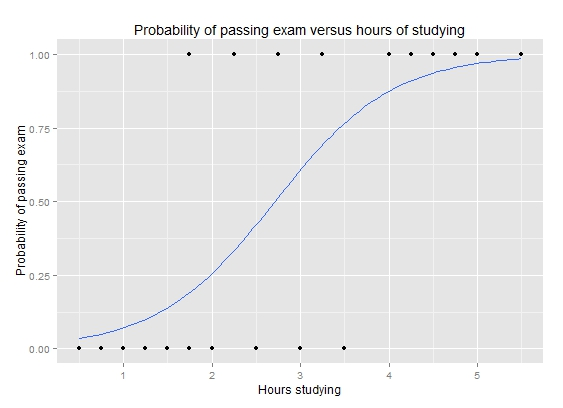
\includegraphics[width=0.8\textwidth]{figures/regression/Exam_pass_logistic_curve.jpeg}
\caption{
Example logistic regression curve on one input feature, by \href{https://en.wikipedia.org/wiki/File:Exam_pass_logistic_curve.jpeg}{Michaelg2015}.
}
\label{fig:logistic_regression_ex}
\end{figure}

Some assumptions of the logistic regression approach are:
\begin{enumerate}[noitemsep]
\item $y$ is either present or absent (dichotomous).
\item There are minimal correlations between the $x_{j}$ features (no multicollinearity).
\item There are no major outliers in the data.
\end{enumerate}

% TODO pseudo R2, Wald statistic

%%%%%%%%%%%%%%%%%%%%%%%%%%%%%%%%%%%%%%%%%%%%%%%%%%%%%%%%
%%%%%%%%%%%%%%%%%%%%%%%%%%%%%%%%%%%%%%%%%%%%%%%%%%%%%%%%
\section{Gaussian Process Regression}
\label{Regression:kriging}
% TODO also known as kriging

}
%%%%%%%%%%%%%%%%%%%%%%%%%%%%%%%%%%%%%%%%%%%%%%%%%%%%%%%%
%%%%%%%%%%%%%%%%%%%%%%%%%%%%%%%%%%%%%%%%%%%%%%%%%%%%%%%%
%%%%%%%%%%%%%%%%%%%%%%%%%%%%%%%%%%%%%%%%%%%%%%%%%%%%%%%%
% \chapter{Machine Learning}
% \label{ml}

%%%%%%%%%%%%%%%%%%%%%%%%%%%%%%%%%%%%%%%%%%%%%%%%%%%%%%%%
%%%%%%%%%%%%%%%%%%%%%%%%%%%%%%%%%%%%%%%%%%%%%%%%%%%%%%%%
%%%%%%%%%%%%%%%%%%%%%%%%%%%%%%%%%%%%%%%%%%%%%%%%%%%%%%%%
\chapter{General Machine Learning Concepts}
\label{ml:general}

%%%%%%%%%%%%%%%%%%%%%%%%%%%%%%%%%%%%%%%%%%%%%%%%%%%%%%%%
%%%%%%%%%%%%%%%%%%%%%%%%%%%%%%%%%%%%%%%%%%%%%%%%%%%%%%%%
\section{Evaluating Performance}
\label{ml:general:eval}

%%%%%%%%%%%%%%%%%%%%%%%%%%%%%%%%%%%%%%%%%%%%%%%%%%%%%%%%
\subsection{Confusion Matrix}
\label{ml:general:eval:cm}

The confusion matrix is a simple table of the number of actual, or truth, class instances
versus the number of a model's predicted class instances.
A two class example is provided in \cref{table:CM}.
Multi-class confusion matrices are straight forward extensions,
with correctly classified instances appearing along the diagonal.

\begin{table}[H]
  \centering
  \begin{tabular}{c | c | c | c |}
  \multicolumn{2}{c}{} & \multicolumn{2}{c}{\textbf{Actual}} \\ \cline{3-4}
  \multicolumn{1}{c}{} & & Positive & Negative \\ \cline{2-4}
  \multirow{4}{*}{\rotatebox{90}{\textbf{Predicted}}} & \multirow{2}{*}{Positive} & \multirow{2}{*}{TP} & FP \\[-8pt]
   & & & (Type I) \\ \cline{2-4}
   & \multirow{2}{*}{Negative} & FN & \multirow{2}{*}{TN} \\[-8pt]
   & & (Type II) & \\ \cline{2-4}
  \end{tabular}
  \caption{Two class confusion matrix.}
  \label{table:CM}
\end{table}

%%%%%%%%%%%%%%%%%%%%%%%%%%%%%%%%%%%%%%%%%%%%%%%%%%%%%%%%
\subsection{TPR \& TNR -- Sensitivity \& Specificity}
\label{ml:general:eval:TPR_TNR}

The true positive rate (TPR) and true negative rate (TNR) are
relatively straight forward to compute and understand, along with their complements,
the false negative rate (FNR), \ie miss rate, and false positive rate (FPR), \ie fall-out.
Here the denominators are the number of true class members.

\begin{enumerate}[noitemsep]
\item True positive rate (TPR), \ie sensitivity, recall, hit rate:
\begin{equation} \label{eq:TPR}
\text{TPR} = \frac{\text{TP}}{\text{P}} = \frac{\text{TP}}{\text{TP}+\text{FN}} = 1 - \text{FNR} = P\left(\hat{+} \mid + \right)
\end{equation}

\item True negative rate (TNR), \ie specificity, selectivity:
\begin{equation} \label{eq:TNR}
\text{TNR} = \frac{\text{TN}}{\text{N}} = \frac{\text{TN}}{\text{TN}+\text{FP}} = 1 - \text{FPR} = P\left(\hat{-} \mid - \right)
\end{equation}
\end{enumerate}

%%%%%%%%%%%%%%%%%%%%%%%%%%%%%%%%%%%%%%%%%%%%%%%%%%%%%%%%
\subsection{PPV (Precision) \& NPV}
\label{ml:general:eval:PPV_NPV}

The positive predictive value (PPV), more commonly known as precision, and negative predictive value (NPV)
are related metrics, but with predicted class members in the denominators.
Their complements are the false discovery rate (FDR) and false omission rate (FOR).
It is helpful to look at these metrics graphically, as in \cref{fig:graphical_CM_quantities}.

\begin{enumerate}[noitemsep]
\item Positive predictive value (PPV), \ie precision:
\begin{equation} \label{eq:PPV}
\text{PPV} = \frac{\text{TP}}{\hat{\text{P}}} = \frac{\text{TP}}{\text{TP}+\text{FP}} = 1 - \text{FDR} = P\left(+ \mid \hat{+} \right)
\end{equation}

\item Negative predictive value (NPV):
\begin{equation} \label{eq:NPV}
\text{NPV} = \frac{\text{TN}}{\hat{\text{N}}} = \frac{\text{TN}}{\text{TN}+\text{FN}} = 1 - \text{FOR} = P\left(- \mid \hat{-} \right)
\end{equation}
\end{enumerate}

\begin{figure}[H]
\centering
  \begin{subfigure}[c]{0.48\textwidth}\centering
  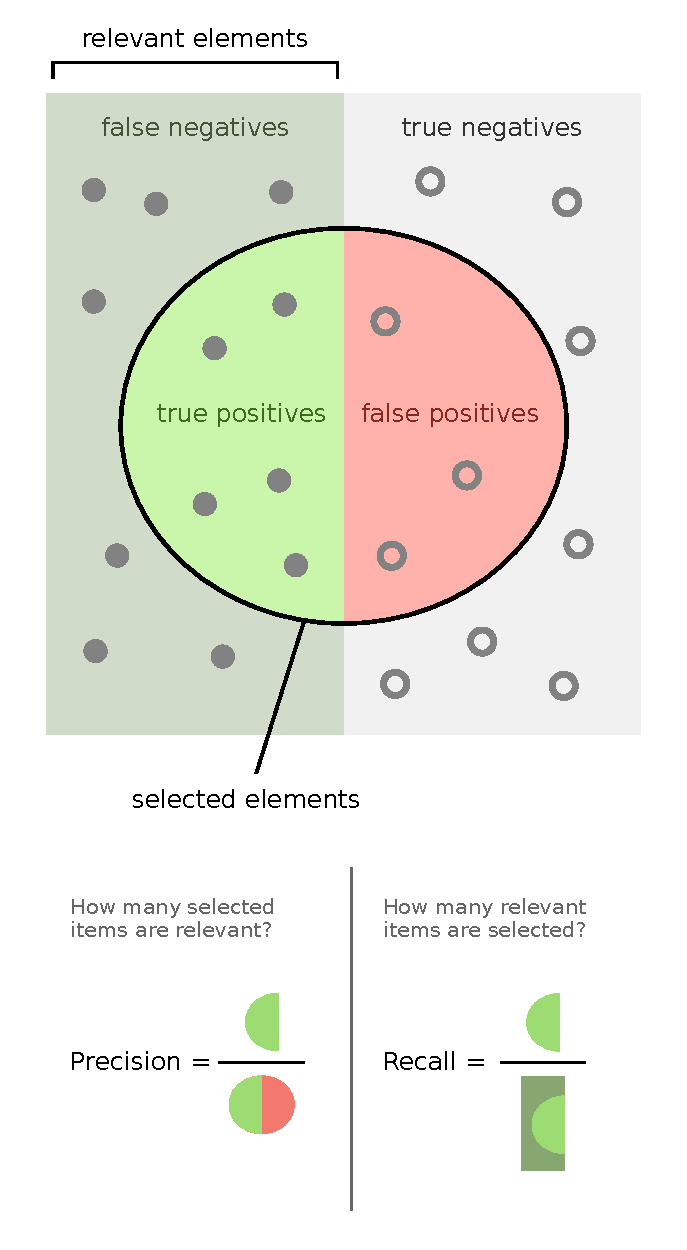
\includegraphics[width=\textwidth]{figures/ml/precision_recall.pdf}
  \caption{Precision \& Recall}
  \label{fig:graphical_CM_quantities:precision_recall}
  \end{subfigure}
  ~
  \begin{subfigure}[c]{0.48\textwidth}\centering
  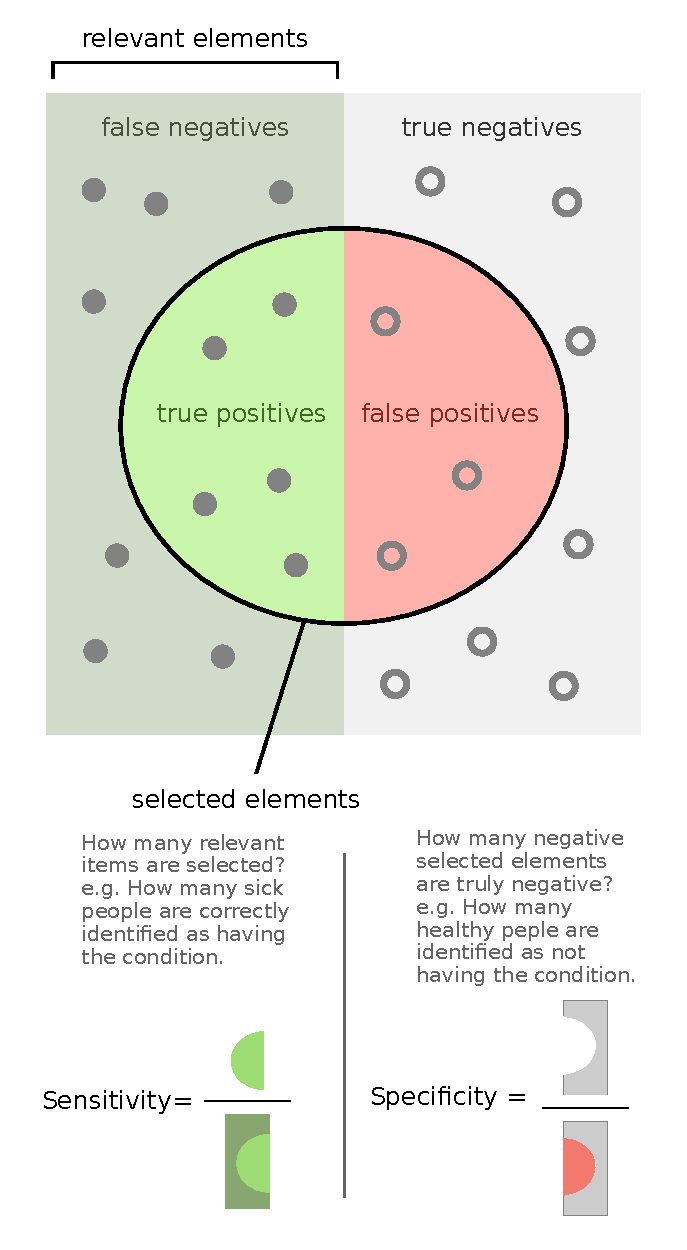
\includegraphics[width=\textwidth]{figures/ml/sensitivity_and_specificity.pdf}
  \caption{Sensitivity \& Specificity}
  \label{fig:graphical_CM_quantities:sensitivity_specificity}
  \end{subfigure}
\caption{
Graphical representation of
precision versus recall (sensitivity), by \href{https://commons.wikimedia.org/wiki/File:Precisionrecall.svg}{Walber},
and
sensitivity (recall) versus specificity, by \href{http://en.wikipedia.org/wiki/File:Sensitivity_and_specificity.svg}{FeanDoe}.
}
\label{fig:graphical_CM_quantities}
\end{figure}

%%%%%%%%%%%%%%%%%%%%%%%%%%%%%%%%%%%%%%%%%%%%%%%%%%%%%%%%
\subsection{Other Scores}
\label{ml:general:eval:other_scores}

The accuracy (ACC), the proportion of correct predictions, is a natural metric for measuring a classifiers performance.
Various F-scores, such as $F_{1}$ and $F_{\beta}$, combine precision and recall into one metric\footnote{Note that $F_{\beta}$ does not depend on TN at all, a potential shortcoming.}.
$F_{1}$ balances precision and recall equally, and is their harmonic mean,
while $F_{\beta}$ uses $\beta$ to assign different weights to each\footnote{$F_{2}$ weights recall over precision, $F_{0.5}$ weights precision over recall.}.

\begin{enumerate}[noitemsep]
\item Accuracy (ACC):
\begin{equation} \label{eq:ACC}
\text{ACC} = \frac{\text{TP}+\text{TN}}{\text{P}+\text{N}} = \frac{\text{TP}+\text{TN}}{\text{TP}+\text{TN}+\text{FP}+\text{FN}}
\end{equation}

\item $F_{1}$ ($F_{1}=1$ is best, $F_{1}=0$ is worst):
\begin{equation} \label{eq:F1}
F_{1} = \left(\frac{\text{precision}^{-1}+\text{recall}^{-1}}{2}\right)^{-1} = 2\,\,\frac{\text{precision} \times \text{recall}}{\text{precision} + \text{recall}}
\end{equation}

\item $F_{\beta}$ (Larger $\beta$ weights recall over precision):
\begin{equation} \label{eq:Fbeta}
F_{\beta} = \left(1+\beta^{2}\right) \frac{\text{precision} \times \text{recall}}{\beta^{2}\,\text{precision} + \text{recall}} =
\frac{\left(1+\beta^{2}\right) \text{TP}}{\left(1+\beta^{2}\right) \text{TP} + \beta^{2}\,\text{FN} + \text{FP}}
\end{equation}
\end{enumerate}

\clearpage% TODo hard coded
%%%%%%%%%%%%%%%%%%%%%%%%%%%%%%%%%%%%%%%%%%%%%%%%%%%%%%%%
%%%%%%%%%%%%%%%%%%%%%%%%%%%%%%%%%%%%%%%%%%%%%%%%%%%%%%%%
\section{Bias-Variance Tradeoff}
\label{ml:general:bias_variance_tradeoff}

\begin{enumerate}[noitemsep]
\item Bias: Errors due to a model not learning about relationships between features in the training data, \ie underfitting. Caused by invalid relationships present in the model.
\item Variance: Errors due to an overly complex model failing to generalize beyond the training data, \ie overfitting. Caused by sensitivity to small fluctuations in the training data.
\end{enumerate}

\begin{figure}[H]
  \centering
  \savebox{\largestimage}{
    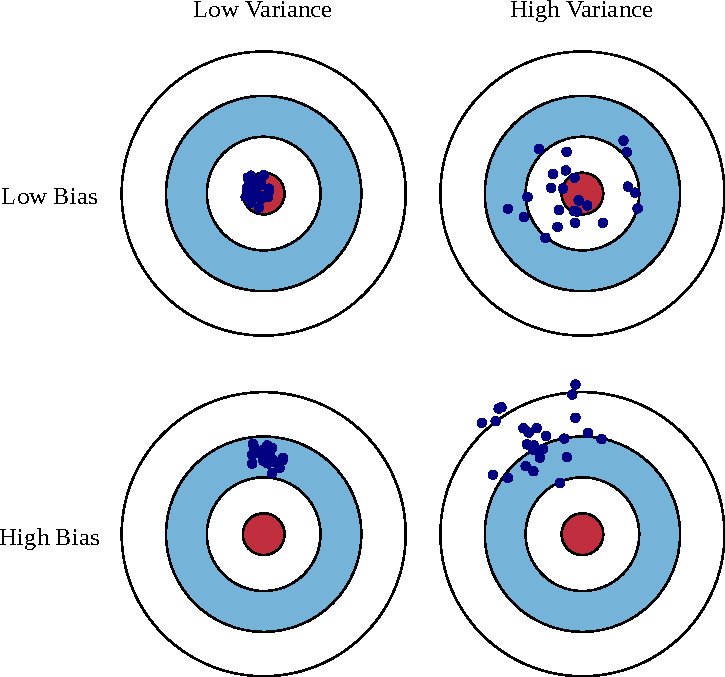
\includegraphics[width=0.47\textwidth]{figures/ml/bias_variance_tradeoff.pdf}
  }% Store largest image in a box

  \begin{subfigure}[b]{0.48\textwidth}\centering
    \usebox{\largestimage}
    \vspace{0.01cm}
  \caption{Direct Comparison}
  \label{fig:ml:bias_variance_tradeoff:direct}
  \end{subfigure}
  ~
  \begin{subfigure}[b]{\wd\largestimage}\centering
    \raisebox{\dimexpr.5\ht\largestimage-.5\height}{% Adjust vertical height of smaller image
      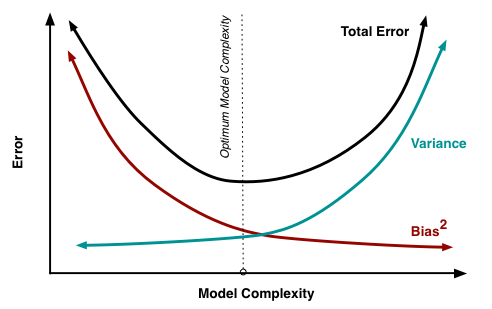
\includegraphics[width=\textwidth]{figures/ml/bias_variance_error_tradeoff.png}}
  \caption{Error Components (Test Set)}
  \label{fig:ml:bias_variance_tradeoff:error}
  \end{subfigure}
\caption{
Illustrations of the bias-variance tradeoff,
by \href{http://scott.fortmann-roe.com/docs/BiasVariance.html}{Scott Fortmann-Roe}.
\label{fig:ml:bias_variance_tradeoff}
}
\end{figure}

Every model makes a tradeoff between bias and variance,
which is roughly controlled by its level of complexity
as can be seen in \cref{fig:ml:bias_variance_tradeoff:error}.
\Cref{fig:additional:ml:general:early_stopping} shows this in practice,
as past a certain point of complexity the validation error grows
while the training error continues to decrease.

\subsubsection{Mean Square Error (MSE) Decomposition}
\label{ml:general:bias_variance_tradeoff:decop}

We can analytically decompose the mean square error (MSE) into explicit
bias, variance, and irreducable error components.
Let $y = f\left(\mathbf{x}\right) + \epsilon$ represent
the observed data, $y_{i}$, $\mathbf{x}_{i}$,
where $f\left(\mathbf{x}\right)$ is the true parent distribution\footnote{$\expval{f} = f$ is deterministic,
and acts as a constant as far as expectation values are concerned.} and
$\epsilon$ is random noise\footnote{This is the source of the irreducible error.
Since future data will still have $\epsilon$, the predictions can't be perfect
-- even when neglecting the model's own bias and variance.}\footnote{Later we'll need
$\sigma^{2} = \variance{\epsilon} = \expval{\epsilon^{2}} - \expval{\epsilon}^{2} = \expval{\epsilon^{2}}$.} having
$\expval{\epsilon} = 0$, $\variance{\epsilon} = \sigma^{2}$.
Representing the trained model\footnote{Note
that $\cov{\epsilon}{\hat{f}} = 0 \Rightarrow \expval{\epsilon \hat{f}} = \expval{\epsilon} \expval{\hat{f}}$.} as
$\hat{f}\left(\mathbf{x}\right)$, we expand the MSE:

\begin{subequations} \label{eq:bias_variance_tradeoff:decop}
\begin{align}
\text{MSE} &= \expval{\left(y-\hat{f}\right)^{2}} \\
&= \expval{\left(f + \epsilon - \hat{f} + \big[\expval{\hat{f}}-\expval{\hat{f}}\big]\right)^{2}}\,, \\
&= \expval{\left(\big[f - \expval{\hat{f}}\big] + \epsilon - \big[\hat{f} - \expval{\hat{f}}\big]\right)^{2}}\,, \\
&= \expval{\left(f-\expval{\hat{f}}\right)^{2}}
+\expval{\epsilon^{2}}
+\expval{\left(\hat{f}-\expval{\hat{f}}\right)^{2}}
+2\expval{\left(f-\expval{\hat{f}}\right)\epsilon} \\
&\hphantom{=}-2\expval{\epsilon\left(\hat{f}-\expval{\hat{f}}\right)}
-2\expval{\left(f-\expval{\hat{f}}\right)\left(\hat{f}-\expval{\hat{f}}\right)}\,, \\
&= \left(-1\right)^{2}\left(\expval{\hat{f}}-f\right)^{2} +\sigma^{2} + \variance{\hat{f}}
+2\left(f-\expval{\hat{f}}\right)\cancelto{0}{\expval{\epsilon}} \\
&\hphantom{=}-2\cancelto{0}{\expval{\epsilon}}\left(\expval{\hat{f}}-\expval{\hat{f}}\right)
-2\left(f-\expval{\hat{f}}\right)\cancelto{0}{\left(\expval{\hat{f}}-\expval{\hat{f}}\right)}\,, \\
&= \left(\bias{\hat{f}}\right)^{2} + \variance{\hat{f}} + \sigma^{2}\,.
\end{align}
\end{subequations}

\clearpage% TODo hard coded
%%%%%%%%%%%%%%%%%%%%%%%%%%%%%%%%%%%%%%%%%%%%%%%%%%%%%%%%
%%%%%%%%%%%%%%%%%%%%%%%%%%%%%%%%%%%%%%%%%%%%%%%%%%%%%%%%
\section{Regularization}
\label{ml:general:reg}

Regularization is a method for controlling the variance (overfitting)
of a model by putting constraints on the size of its parameters.
In terms of \cref{ml:general:bias_variance_tradeoff}, regularization forces the model's
bias to grow on the training set in order to lower the variance on future data.
The two main types of regularization are shown in \cref{eq:L1_L2}
and depend on different powers of the norm\footnote{In
the case of OLS linear regression the constant intercept term $\beta_{0}$ is not included in $\norm{\bm{\beta}}$.} of the model parameters $\bm{\beta}$.
In order to treat all features equally, normalization must be used before applying regularization.
A hyperparameter $\lambda$ is included to tune the amount of regularization applied in the objective function,
$S\left(\bm{\beta}\right) = L + \Omega$.
As $\lambda$ is increased, it decreases the size the model's coefficients, and thereby its variance (overfitting),
up to a point when the model is unable to adequately train on the available data and the bias (underfitting) begins to grow.

\begin{subequations} \label{eq:L1_L2}
\begin{align}
\Omega_{\text{L1}}\left(\bm{\beta}\right) &= \lambda \norm{\bm{\beta}}\hphantom{^{1}}
= \lambda \sum_{j=1}^{n} \, \abs{\beta_{j}}\,, \label{eq:L1} \\
\Omega_{\text{L2}}\left(\bm{\beta}\right) &= \lambda \norm{\bm{\beta}}^{2}
= \lambda \sum_{j=1}^{n} \,\, \beta_{j}^{2}\,. \label{eq:L2}
\end{align}
\end{subequations}

For a particular value of $\lambda$, the effect of L1 and L2 regularization\footnote{Here
$q$ is being used as the power of $\norm{\bm{\beta}}$. For L1 (L2), $q=1$ ($q=2$).} is
to constrain $\norm{\bm{\beta}}^{q} \leq t\left(\lambda\right)$ for some $t\left(\lambda\right)$.
As can be seen in \cref{fig:ml:l1l2} the L1 norm constrains $\bm{\beta}$ to lie within a hypercube,
while the L2 constraint is a hypersphere.

\begin{figure}[H]
  \centering
  \begin{subfigure}[b]{0.48\textwidth}\centering
      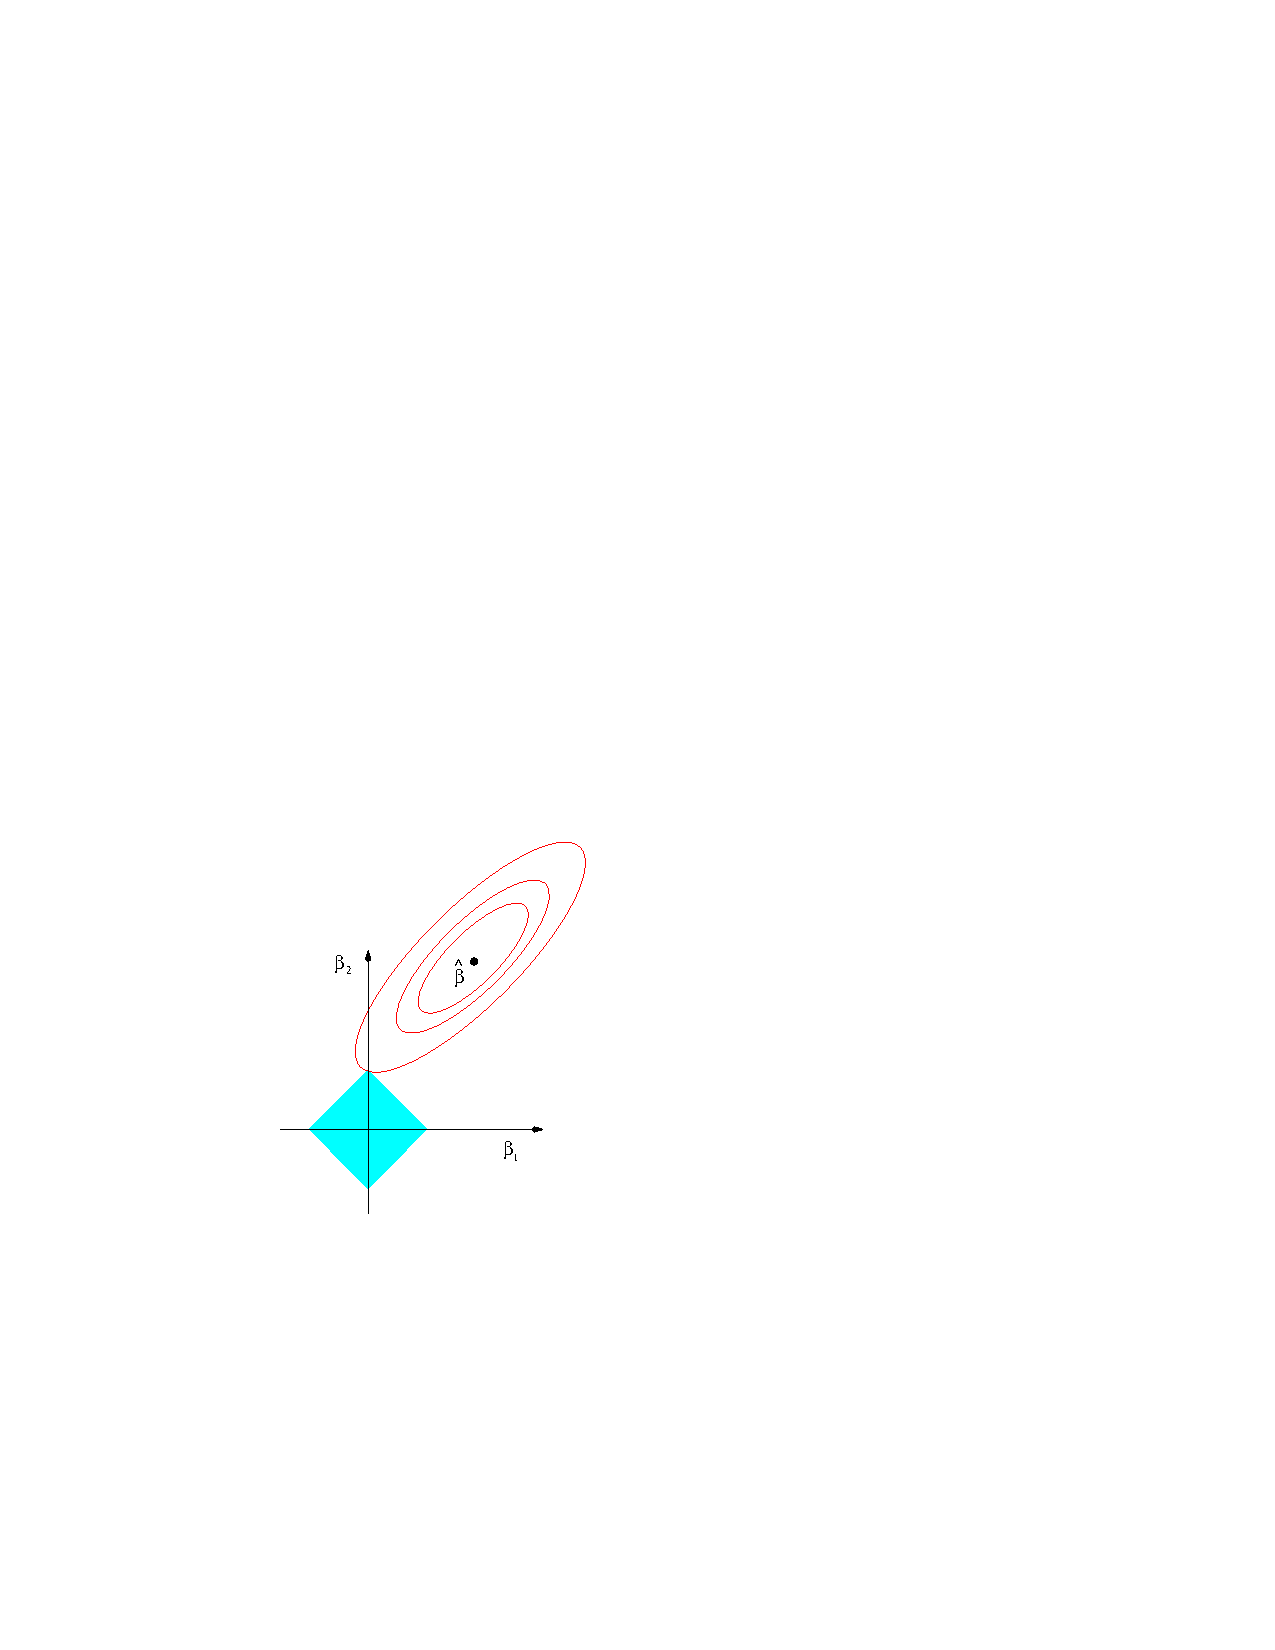
\includegraphics[width=\textwidth]{figures/ml/l1.pdf}
  \caption{L1}
  \label{fig:ml:l1l2:l1}
  \end{subfigure}
  ~
  \begin{subfigure}[b]{0.48\textwidth}\centering
      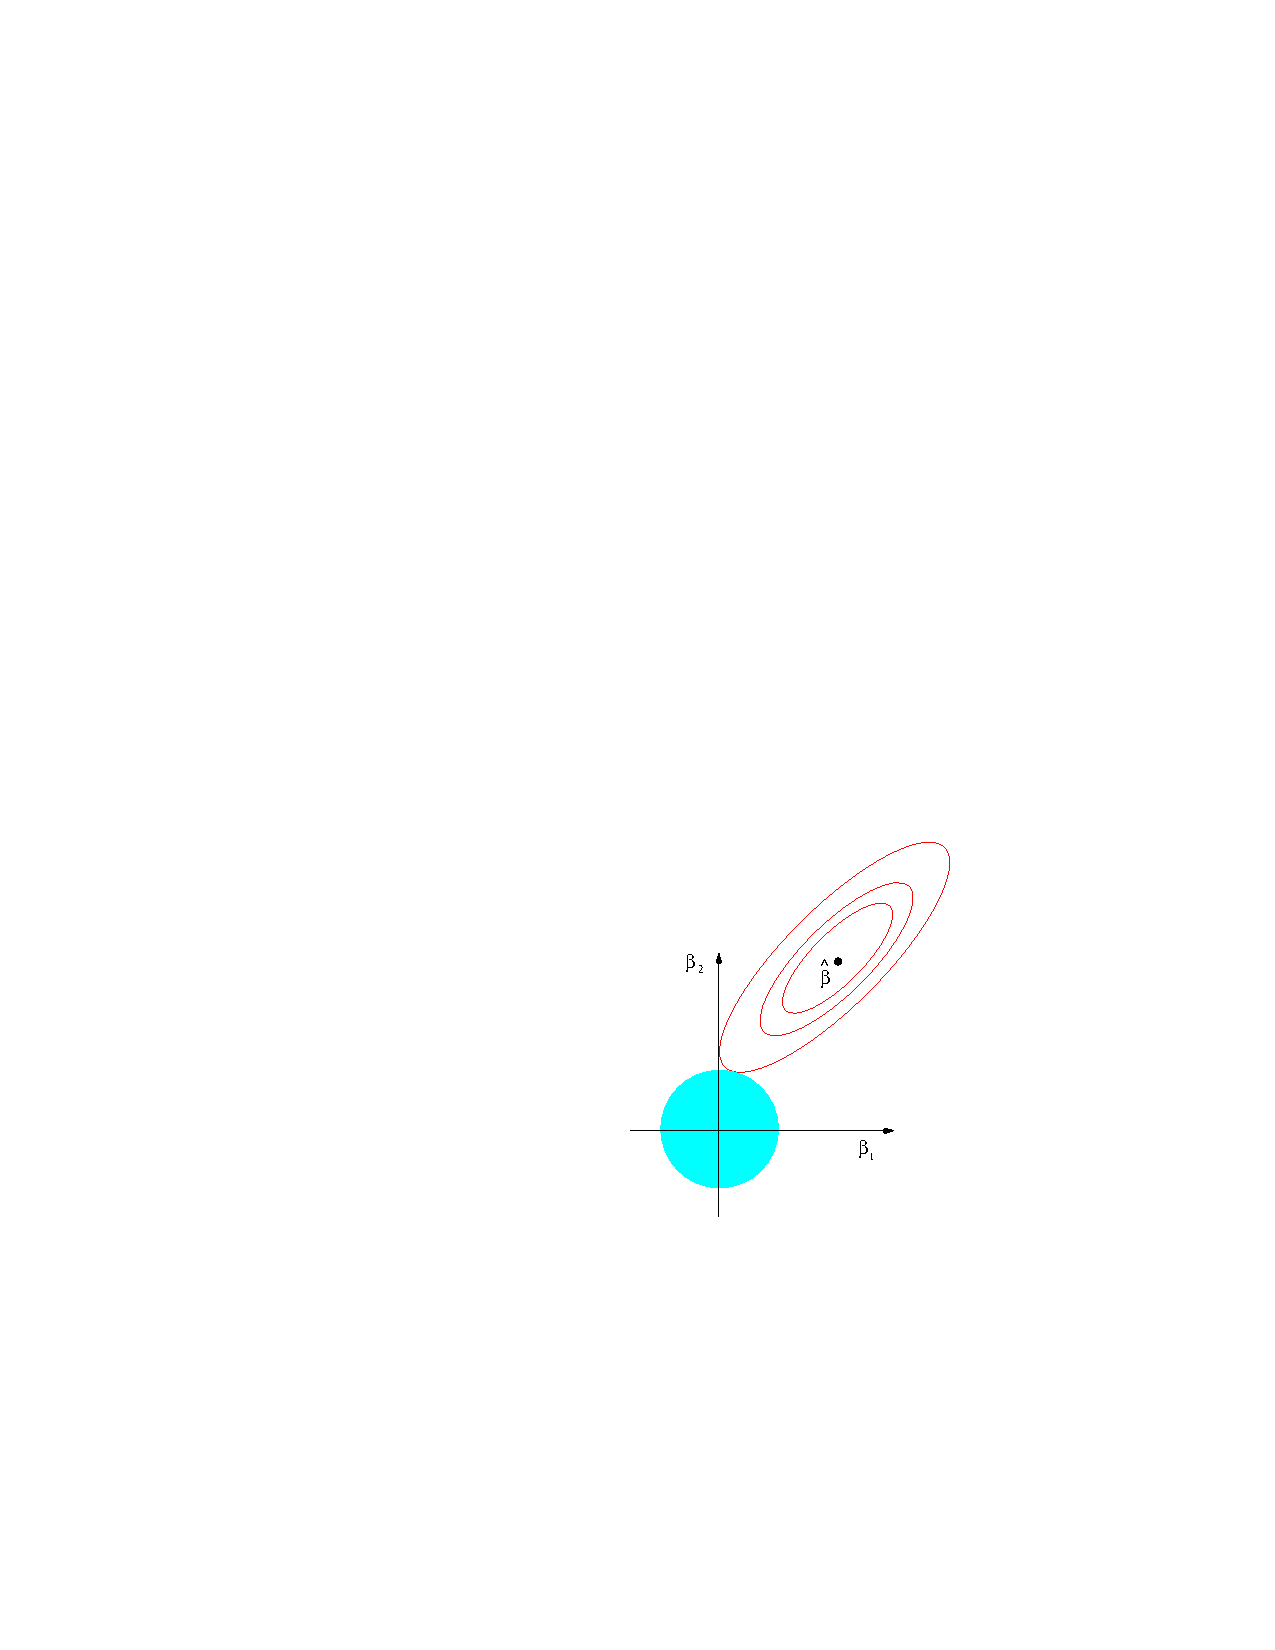
\includegraphics[width=\textwidth]{figures/ml/l2.pdf}
  \caption{L2}
  \label{fig:ml:l1l2:L2}
  \end{subfigure}
\caption{
A graphical representation of the L1 and L2 regularization constraints on $\bm{\beta}$ \cite{HastieTF09}.
The best value of $\bm{\beta}$ for optimizing the loss function $L$ is indicated as $\hat{\bm{\beta}}$.
For a given contour in $L$, L1 will tend to force $\bm{\beta}$ along one of the axes,
identically setting some $\beta_{i}$ coefficients to zero,
while L2 is rotationally symmetric and has no such tendencies.
\label{fig:ml:l1l2}
}
\end{figure}

%%%%%%%%%%%%%%%%%%%%%%%%%%%%%%%%%%%%%%%%%%%%%%%%%%%%%%%%
\subsection{L1 -- LASSO}
\label{ml:general:reg:L1}
L1, or LASSO\footnote{Least absolute shrinkage and selection operator.},
regularization uses the norm $\norm{\bm{\beta}}$ \cref{eq:L1}, or taxi cab distance.
As it's geometric constraints on $\bm{\beta}$ are hypercubes,
it tends to set some model parameters to 0, creating sparsity,
and thereby acts as a form of built-in feature selection.

%%%%%%%%%%%%%%%%%%%%%%%%%%%%%%%%%%%%%%%%%%%%%%%%%%%%%%%%
\subsection{L2 -- Ridge}
\label{ml:general:reg:L2}
L2, or ridge, regularization \cref{eq:L2} uses the square of the norm, or euclidean distance.
Models made with L2 regularization are somewhat less interpretable than those made with L1,
as L2 may make many parameters very small, but does not remove them entirely.
The parameters are still shrunk toward zero, and each other,
while highly correlated features are effectively averaged.
L2 is slightly faster to run than L1 computationally as, unlike L1, it
is not represented as a piecewise function and has a closed form expression.

%%%%%%%%%%%%%%%%%%%%%%%%%%%%%%%%%%%%%%%%%%%%%%%%%%%%%%%%
%%%%%%%%%%%%%%%%%%%%%%%%%%%%%%%%%%%%%%%%%%%%%%%%%%%%%%%%
\section{Gradient Descent}
\label{ml:general:grad_descent}
% TODO

%%%%%%%%%%%%%%%%%%%%%%%%%%%%%%%%%%%%%%%%%%%%%%%%%%%%%%%%
\subsection{Stochastic Gradient Descent (SGD)}
\label{ml:general:grad_descent:stochastic}
% TODO


%%%%%%%%%%%%%%%%%%%%%%%%%%%%%%%%%%%%%%%%%%%%%%%%%%%%%%%%
%%%%%%%%%%%%%%%%%%%%%%%%%%%%%%%%%%%%%%%%%%%%%%%%%%%%%%%%
%%%%%%%%%%%%%%%%%%%%%%%%%%%%%%%%%%%%%%%%%%%%%%%%%%%%%%%%
\chapter{Unsupervised Learning}
\label{ml:unsupervised}

%%%%%%%%%%%%%%%%%%%%%%%%%%%%%%%%%%%%%%%%%%%%%%%%%%%%%%%%
%%%%%%%%%%%%%%%%%%%%%%%%%%%%%%%%%%%%%%%%%%%%%%%%%%%%%%%%
\section{\texorpdfstring{$k$}{k}-Means}
\label{ml:unsupervised:kMean}
% TODO

%%%%%%%%%%%%%%%%%%%%%%%%%%%%%%%%%%%%%%%%%%%%%%%%%%%%%%%%
\subsection{Metrics}
\label{ml:unsupervised:kMean:metrics}
% TODO describe both cartesian and cosine similarity metrics


%%%%%%%%%%%%%%%%%%%%%%%%%%%%%%%%%%%%%%%%%%%%%%%%%%%%%%%%
%%%%%%%%%%%%%%%%%%%%%%%%%%%%%%%%%%%%%%%%%%%%%%%%%%%%%%%%
\section{Supervised Learning}
\label{ml:supervised}

%%%%%%%%%%%%%%%%%%%%%%%%%%%%%%%%%%%%%%%%%%%%%%%%%%%%%%%%
% \subsection{N{\"a}ive Bayes Classification}
% \label{ml:supervised:Bayes}
% TODO

%%%%%%%%%%%%%%%%%%%%%%%%%%%%%%%%%%%%%%%%%%%%%%%%%%%%%%%%
% \subsection{Support Vector Machines (SVM)}
% \label{ml:supervised:SVM}
% TODO

%%%%%%%%%%%%%%%%%%%%%%%%%%%%%%%%%%%%%%%%%%%%%%%%%%%%%%%%
% \subsection{Boosted Decision Trees (BDT)}
% \label{ml:supervised:BDT}
% TODO

% \subsubsection{\xgboost}
% \label{ml:supervised:BDT:xgboost}
% \xgboost \cite{xgboost}
% TODO see https://towardsdatascience.com/boosting-algorithm-xgboost-4d9ec0207d

%\subsubsection{AdaBoost}
%\label{ml:supervised:BDT:AdaBoost}
% TODO

%%%%%%%%%%%%%%%%%%%%%%%%%%%%%%%%%%%%%%%%%%%%%%%%%%%%%%%%
% \subsection{Random Forest}
% \label{ml:supervised:RF}
% TODO

%%%%%%%%%%%%%%%%%%%%%%%%%%%%%%%%%%%%%%%%%%%%%%%%%%%%%%%%
% \subsection{Artificial Neural Networks (NN)}
% \label{ml:supervised:ANN}
% TODO

%%%%%%%%%%%%%%%%%%%%%%%%%%%%%%%%%%%%%%%%%%%%%%%%%%%%%%%%
% \subsection{Recursive Neural Networks (RNN)}
% \label{ml:supervised:RNN}
% TODO

% \subsubsection{Long Short Term Memory (LSTM)}
% \label{ml:supervised:RNN:LSTM}
% TODO

%%%%%%%%%%%%%%%%%%%%%%%%%%%%%%%%%%%%%%%%%%%%%%%%%%%%%%%%
% \subsection{Convolutional Neural Networks (CNN)}
% \label{ml:supervised:CNN}
% TODO

%%%%%%%%%%%%%%%%%%%%%%%%%%%%%%%%%%%%%%%%%%%%%%%%%%%%%%%%
% \subsection{Adversarial Networks (AN?)}
% \label{ml:supervised:AN}
% TODO

%%%%%%%%%%%%%%%%%%%%%%%%%%%%%%%%%%%%%%%%%%%%%%%%%%%%%%%%
% \subsection{Variational Autoencoders (VAE)}
% \label{ml:supervised:VAE}
% TODO

%%%%%%%%%%%%%%%%%%%%%%%%%%%%%%%%%%%%%%%%%%%%%%%%%%%%%%%%
% \subsection{$k$-Nearest Neighbors ($k$-NN)}
% \label{ml:supervised:kNN}
% TODO

% \subsection{Learning Vector Quantization (LVQ)}
% \label{ml:supervised:kNN:LVQ}
% TODO


}
\chapter{Miscellaneous}
\label{chap:misc}

%%%%%%%%%%%%%%%%%%%%%%%%%%%%%%%%%%%%%%%%%%%%%%%%%%%%%%%%
\section{Feature Importance}
\label{misc:feature_importance}
% TODO

%%%%%%%%%%%%%%%%%%%%%%%%%%%%%%%%%%%%%%%%%%%%%%%%%%%%%%%%
\section{Experimental Design \& Hypothesis Testing}
\label{misc:exp_design}
% TODO

%%%%%%%%%%%%%%%%%%%%%%%%%%%%%%%%%%%%%%%%%%%%%%%%%%%%%%%%
\section{Dimensionality Reduction}
\label{misc:m_reduction}
% TODO

%%%%%%%%%%%%%%%%%%%%%%%%%%%%%%%%%%%%%%%%%%%%%%%%%%%%%%%%
\section{Factor Analysis}
\label{misc:factor_ana}
% TODO

}

%==============================================================================

%-----------------------------------------------------------------------------%
% APPENDICES -- OPTIONAL. These are just chapters enumerated by Appendix A, Appendix B, Appendix C...
%-----------------------------------------------------------------------------%
% Start each appendix tex file with '\chapter{Title}'
\appendix
%%%%%%%%%%%%%%%%%%%%%%%%%%%%%%%%%%%%%%%%%%%%%%%%%%%%%%%%
%%%%%%%%%%%%%%%%%%%%%%%%%%%%%%%%%%%%%%%%%%%%%%%%%%%%%%%%
%%%%%%%%%%%%%%%%%%%%%%%%%%%%%%%%%%%%%%%%%%%%%%%%%%%%%%%%
\chapter{\pandas}
\label{pandas}

%%%%%%%%%%%%%%%%%%%%%%%%%%%%%%%%%%%%%%%%%%%%%%%%%%%%%%%%
%%%%%%%%%%%%%%%%%%%%%%%%%%%%%%%%%%%%%%%%%%%%%%%%%%%%%%%%
\section{Basic Commands}
\label{pandas:basic}

\begin{lstlisting}[language=Python]
# IO
df = pd.read_csv('file.csv', header=None)
df['col'] = df['col'].astype(int)
df.to_csv('out.csv')

# descriptive commands
df.describe(); df.columns; df.shape;

# aggregation commands
df.sum(); df.cumsum();
df.min(); df.max(); df.idxmin(); df.idxmax();
df.mean(); df.std(); df.median(); df.mode();

# extract all rows from one column
df_y = df.loc[:, ['y']]

# select by value
df_selection = df.loc[( ((df['x'] == x_value) & (df['y'] == y_value)) | (df['z'] > z_value))]

# select by value and assign new value
df.loc[(df['x'] == x_value), 'y'] = y_value

# select with query
df_selection = df.query('x > 0')

# select with isin
df_selection = df.isin({'x': [x_value1, x_value2], 'y': [y_value]})

# select row by index
series = df.iloc[0]

# apply an arbitrary function
def func(x, y):
  return x*np.sin(y)
df['z'] = np.vectorize(func)(df['x'], df['y'])

# iterate through rows (slow!)
for index, row in df.iterrows():
  x_value = row['x']

# construct from rows
rows_list = []
for nrow in range(nrows):
  rows_list.append({'x':x_value, 'y':y_value})
df = pd.DataFrame(rows_list)
df = df[['x', 'y']]

# rename columns
df = df.rename({'old': 'new'}, axis='columns')

# sort
df = df.sort_values(by=['x', 'y'], ascending=[True, False]).reset_index(drop=True)

# group by, while dropping new count column and duplicates
df = df.groupby(['x', 'y', 'z']).size().to_frame(name = 'count').reset_index().drop(['count'], axis=1).drop_duplicates()

# return duplicate rows
columns_to_check_for_duplicates = ['x', 'y']
df_duplicates = df[df.duplicated(subset=columns_to_check_for_duplicates, keep=False)]

# shuffling
df = df.sample(frac=1., replace=False, random_state=rnd_seed).reset_index(drop=True)

# drop columns
df = df.drop(['col_to_drop1', 'col_to_drop2'], axis=1)

# fill nans, for all columns and per column
df = df.fillna(0.0)
df = df.fillna(value={'x': x_nan_value, 'z': y_nan_value})
\end{lstlisting}

\clearpage

%%%%%%%%%%%%%%%%%%%%%%%%%%%%%%%%%%%%%%%%%%%%%%%%%%%%%%%%
%%%%%%%%%%%%%%%%%%%%%%%%%%%%%%%%%%%%%%%%%%%%%%%%%%%%%%%%
\section{Joining}
\label{pandas:join}

\noindent See the \href{https://pandas.pydata.org/pandas-docs/stable/user_guide/merging.html}{documentation} and this \href{http://chrisalbon.com/python/data_wrangling/pandas_join_merge_dataframe/}{useful guide}.

\begin{lstlisting}[language=Python]
df = pd.merge(df_l, df_r, left_on='id_left', right_on='id_right', how='left')
\end{lstlisting}

%%%%%%%%%%%%%%%%%%%%%%%%%%%%%%%%%%%%%%%%%%%%%%%%%%%%%%%%
%%%%%%%%%%%%%%%%%%%%%%%%%%%%%%%%%%%%%%%%%%%%%%%%%%%%%%%%
\section{Pivoting}
\label{pandas:pivoting}

\subsubsection{pivot}
\label{pandas:pivoting:pivot}

\noindent \href{http://pandas.pydata.org/pandas-docs/stable/reference/api/pandas.DataFrame.pivot.html}{\texttt{pivot} documentation}.

\begin{lstlisting}[language=Python]
DataFrame.pivot(index=None, columns=None, values=None)
\end{lstlisting}

\begin{figure}[H]
\centering
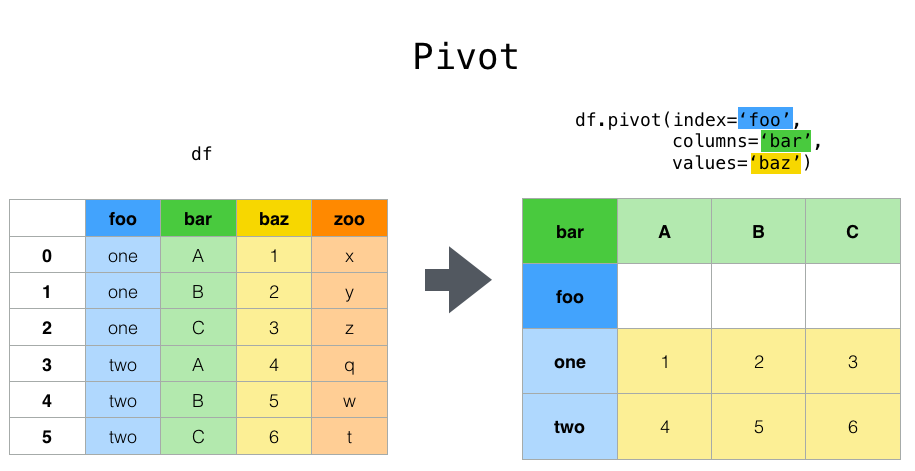
\includegraphics[width=0.85\textwidth]{figures/pandas/reshaping_pivot.png}
\caption{
Example \pandas \texttt{pivot} operation, from the package \href{http://pandas.pydata.org/pandas-docs/stable/user_guide/reshaping.html}{documentation}.
}
\label{fig:pandas:pivot}
\end{figure}

\subsubsection{pivot\_table}
\label{pandas:pivoting:pivot_table}

\noindent \href{https://pandas.pydata.org/pandas-docs/stable/reference/api/pandas.pivot_table.html}{\texttt{pivot\_table} documentation}.

\begin{lstlisting}[language=Python]
pandas.pivot_table(data, values=None, index=None, columns=None, aggfunc='mean', fill_value=None, margins=False, dropna=True, margins_name='All')
\end{lstlisting}

\begin{figure}[H]
\centering
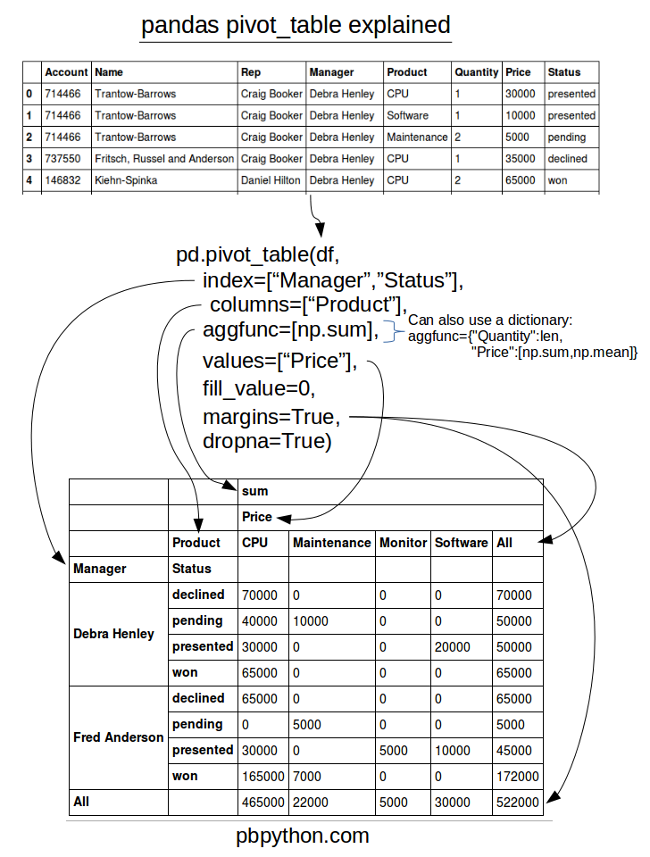
\includegraphics[width=0.95\textwidth]{figures/pandas/pivot-table-datasheet.png}
\caption{
Example \pandas \texttt{pivot\_table} operation, by \href{http://pbpython.com/pandas-pivot-table-explained.html}{Chris Moffitt}.
}
\label{fig:pandas:pivot_table}
\end{figure}
}
%%%%%%%%%%%%%%%%%%%%%%%%%%%%%%%%%%%%%%%%%%%%%%%%%%%%%%%%
%%%%%%%%%%%%%%%%%%%%%%%%%%%%%%%%%%%%%%%%%%%%%%%%%%%%%%%%
\chapter{\sql}
\label{sql}

%%%%%%%%%%%%%%%%%%%%%%%%%%%%%%%%%%%%%%%%%%%%%%%%%%%%%%%%
%%%%%%%%%%%%%%%%%%%%%%%%%%%%%%%%%%%%%%%%%%%%%%%%%%%%%%%%
\section{Basic Commands}
\label{sql:basic}
% TODO

}
%%%%%%%%%%%%%%%%%%%%%%%%%%%%%%%%%%%%%%%%%%%%%%%%%%%%%%%%
%%%%%%%%%%%%%%%%%%%%%%%%%%%%%%%%%%%%%%%%%%%%%%%%%%%%%%%%
%%%%%%%%%%%%%%%%%%%%%%%%%%%%%%%%%%%%%%%%%%%%%%%%%%%%%%%%
\chapter{\pyspark}
\label{pyspark}

%%%%%%%%%%%%%%%%%%%%%%%%%%%%%%%%%%%%%%%%%%%%%%%%%%%%%%%%
%%%%%%%%%%%%%%%%%%%%%%%%%%%%%%%%%%%%%%%%%%%%%%%%%%%%%%%%
\section{Basic Commands}
\label{pyspark:basic}

\begin{lstlisting}[language=Python]
import pyspark.sql.functions as F
from pyspark.sql.window import Window
from pyspark.sql.types import IntegerType, DoubleType

# IO
df = spark.read.parquet('s3a://bucket/table')
df = df.withColumn('col', F.col('col').cast(IntegerType()))
df.write.save('s3a://bucket/table.parquet')

# descriptive commands
df.describe().show(); df.printSchema();
df.show(10); df.limit(10).toPandas();

# select columns
df_y = df.select('x', 'y')

# get distinct values
df_y_distinct = df.select('y').distinct()

# select by value
df_selection = df.where( ((F.col('x') == x_value) & (F.col('y') == y_value)) | (F.col('z') < z_value) )
df_selection = df.where( F.col('x').isNotNull() )

# select by value and assign new value
df = df.withColumn('y', F.when( F.col('x') == x_value, F.lit(y_value) ).otherwise(F.col('y')))

# select where isin, and not (~) isin, some_list
df_selection = df.where(F.col('x').isin(some_list))
df_selection = df.where(~F.col('x').isin(some_list))

# apply an arbitrary function - slow unless written in scala!
def func(x, y):
	return x*np.sin(y)
func_udf = F.udf(func, DoubleType())
df = df.withColumn('z', func_udf('x', 'y'))

# rename columns
df = df.withColumnRenamed('old', 'new')

# order by
df = df.orderBy(['x', 'y'], ascending=[True, False])

# group by, while counting rows and aggregating max date
df = df.groupBy('x', 'y', 'z').agg(F.count('*').alias('count'), F.max('date_col').alias('max_date'))

# group by, get mode of state per patient - deterministically (alphabetical order)
# can be expanded to additional columns, each with their own .join(df.groupBy()...) statements
df.select('patient').distinct().join(
df.where(F.col('state').isNotNull())
	.groupBy(['patient', 'state']).count().alias('c')
	.withColumn('row_num', F.row_number().over(Window().partitionBy('patient').orderBy(F.col('c').desc(), F.col('state'))))
	.where(F.col('row_num') == 1)
	.select('patient', 'state')
, 'patient', 'left')

# return duplicate rows
df.join(df, df.groupBy('x', 'y').agg(F.count('*').alias('c')).where(1 < F.('c')), ['x', 'y'], 'left_semi')

# drop columns
df = df.drop('col_to_drop1', 'col_to_drop2')

cols_to_drop = ['col1', 'col2']
df = df.drop(*cols_to_drop)

# fill nans, for all columns and per column - other syntaxes are also available
df = df.fillna(0.0)
df = df.fillna({'x': x_nan_value, 'z': y_nan_value})

# run a SQL query, note you must register the needed dataframes as tables first
df.registerTempTable('df')
spark.sql('select * from df limit 10').show(10)
\end{lstlisting}

%%%%%%%%%%%%%%%%%%%%%%%%%%%%%%%%%%%%%%%%%%%%%%%%%%%%%%%%
%%%%%%%%%%%%%%%%%%%%%%%%%%%%%%%%%%%%%%%%%%%%%%%%%%%%%%%%
\section{Joining}
\label{pyspark:join}

\noindent See the
\href{https://spark.apache.org/docs/latest/api/python/reference/api/pyspark.sql.DataFrame.join.html#pyspark-sql-dataframe-join}{documentation}
and this
\href{http://www.learnbymarketing.com/1100/pyspark-joins-by-example/}{useful guide}.
In addition to the standard types of joins \texttt{left\_semi}, or \texttt{leftsemi},
is very useful for filtering the left table to the matching rows in the join condition,
without actually joining any columns from the right table.

\begin{lstlisting}[language=Python]
df = df_l.join(df_r, df_l['id_left'] == df_r['id_right'], 'left')
\end{lstlisting}

%%%%%%%%%%%%%%%%%%%%%%%%%%%%%%%%%%%%%%%%%%%%%%%%%%%%%%%%
%%%%%%%%%%%%%%%%%%%%%%%%%%%%%%%%%%%%%%%%%%%%%%%%%%%%%%%%
\section{Pivoting}
\label{pyspark:pivoting}

\noindent \href{https://spark.apache.org/docs/latest/api/python/reference/api/pyspark.sql.GroupedData.pivot.html#pyspark-sql-groupeddata-pivot}{\texttt{pivot} documentation},
and
\href{https://sparkbyexamples.com/pyspark/pyspark-pivot-and-unpivot-dataframe/}{examples}.

\begin{lstlisting}[language=Python]
df.groupBy('product').pivot('state').sum('cost')
\end{lstlisting}
}
%%%%%%%%%%%%%%%%%%%%%%%%%%%%%%%%%%%%%%%%%%%%%%%%%%%%%%%%
%%%%%%%%%%%%%%%%%%%%%%%%%%%%%%%%%%%%%%%%%%%%%%%%%%%%%%%%
%%%%%%%%%%%%%%%%%%%%%%%%%%%%%%%%%%%%%%%%%%%%%%%%%%%%%%%%
\chapter{Coding Concepts}
\label{coding}

%%%%%%%%%%%%%%%%%%%%%%%%%%%%%%%%%%%%%%%%%%%%%%%%%%%%%%%%
%%%%%%%%%%%%%%%%%%%%%%%%%%%%%%%%%%%%%%%%%%%%%%%%%%%%%%%%
\section{Sorting Algorithms}
\label{coding:sorts}

\begin{table}[H]
\centering
\begingroup
\renewcommand*{\arraystretch}{1}
\begin{tabular}{c c c c c c}
\hline
Name & Best & Average & Worst & Memory & Links \\
\hline
\hline
\multirow{2}{*}{Quicksort} & \multirow{2}{*}{$\order{n \log{n}}$} & \multirow{2}{*}{$\order{n \log{n}}$} & \multirow{2}{*}{$\order{n^{2}}$} & $\order{\log{n}}$, avg & \multirow{2}{*}{\href{https://youtu.be/XE4VP_8Y0BU}{Computerphile}, \href{https://youtu.be/SLauY6PpjW4}{HR}} \\
 & & & & $\order{n}$, worst & \\
Merge Sort & $\order{n \log{n}}$ & $\order{n \log{n}}$ & $\order{n \log{n}}$ & $\order{n}$ & \href{https://youtu.be/kgBjXUE_Nwc}{Computerphile}, \href{https://youtu.be/KF2j-9iSf4Q}{HR} \\
Bubble Sort & $\order{n}$ & $\order{n^{2}}$ & $\order{n^{2}}$ & $\order{1}$ & \href{https://youtu.be/kgBjXUE_Nwc}{Computerphile}, \href{https://youtu.be/6Gv8vg0kcHc}{HR} \\
Insertion Sort & $\order{n}$ & $\order{n^{2}}$ & $\order{n^{2}}$ & $\order{1}$ & \href{https://youtu.be/pcJHkWwjNl4}{Computerphile} \\
Heapsort & $\order{n \log{n}}$ & $\order{n \log{n}}$ & $\order{n}$ & $\order{1}$ & \href{https://youtu.be/2DmK_H7IdTo}{Michael Sambol} \\
Bogosort & $\order{n}$ & $\order{\left(n+1\right)!}$ & $\infty$ & $\order{1}$ & --- \\
\hline
\end{tabular}

% TODO add Heapsort, Shellsort, Tree Sort

\endgroup
\caption{
A collection of sorting algorithms with time complexities.
}
\label{tab:sorting_table}
\end{table}

% TODO add heapsort

%%%%%%%%%%%%%%%%%%%%%%%%%%%%%%%%%%%%%%%%%%%%%%%%%%%%%%%%
%%%%%%%%%%%%%%%%%%%%%%%%%%%%%%%%%%%%%%%%%%%%%%%%%%%%%%%%
\section{Other}
\label{coding:other}

%%%%%%%%%%%%%%%%%%%%%%%%%%%%%%%%%%%%%%%%%%%%%%%%%%%%%%%%
\subsection{Binary Tree Search}
\label{coding:other:binary_tree_search}
% TODO
% TODO should probably be moved under BFS or DFS
% https://youtu.be/P3YID7liBug

%%%%%%%%%%%%%%%%%%%%%%%%%%%%%%%%%%%%%%%%%%%%%%%%%%%%%%%%
\subsection{Breadth First Search (BFS)}
\label{coding:other:bfs}
% TODO

\subsubsection{Dijkstra's Algorithm}
\label{coding:other:bfs:dijkstra}
% TODO
% https://youtu.be/GazC3A4OQTE

%%%%%%%%%%%%%%%%%%%%%%%%%%%%%%%%%%%%%%%%%%%%%%%%%%%%%%%%
\subsection{Depth First Search (DFS)}
\label{coding:other:dfs}
% TODO

%%%%%%%%%%%%%%%%%%%%%%%%%%%%%%%%%%%%%%%%%%%%%%%%%%%%%%%%
\subsection{Linked Lists}
\label{coding:other:lls}
% TODO

}
%%%%%%%%%%%%%%%%%%%%%%%%%%%%%%%%%%%%%%%%%%%%%%%%%%%%%%%%
%%%%%%%%%%%%%%%%%%%%%%%%%%%%%%%%%%%%%%%%%%%%%%%%%%%%%%%%
%%%%%%%%%%%%%%%%%%%%%%%%%%%%%%%%%%%%%%%%%%%%%%%%%%%%%%%%
\chapter{Additional Concepts}
\label{additional}

While interesting, the concepts covered here are less likely
to be relevant during the interview process.

%%%%%%%%%%%%%%%%%%%%%%%%%%%%%%%%%%%%%%%%%%%%%%%%%%%%%%%%
%%%%%%%%%%%%%%%%%%%%%%%%%%%%%%%%%%%%%%%%%%%%%%%%%%%%%%%%
\section{Statistics}
\label{additional:stats}

%%%%%%%%%%%%%%%%%%%%%%%%%%%%%%%%%%%%%%%%%%%%%%%%%%%%%%%%
\subsection{Expectation Value and Variance}
\label{additional:stats:expval_and_var}

The expectation value \cref{eq:stats:exp_relations} and variance \cref{eq:stats:var_relations} are introductory, yet essential, statistical measures.
Their definitions and interesting properties are reproduced here for reference.
Note that $s$ is the unbiased sample variance,
and the sample mean $\bar{x}$ has $\mu_{\bar{x}} = \mu$, $\sigma_{\bar{x}} = \sigma / \sqrt{n}$,
where $\mu$ and $\sigma$ are from the parent population.

\begin{subequations}\label{eq:stats:exp_relations}
\begin{align}
\expvalE{X} = \expval{X} &= \sum_{j=1}^{m} x_{j} \, p_{j} = \int_{-\infty}^{\infty} x f\left(x\right) \, \dif x \label{eq:stats:exp_relations:def} \\
\bar{x} = \mu &= \frac{1}{n} \sum_{j=1}^{m} x_{j}\,,\,\text{for uniform}~p_{j} \label{eq:stats:exp_relations:mean} \\
\expval{X+Y} &= \expval{X} + \expval{X} \label{eq:stats:exp_relations:add} \\
\expval{a X} &= a \expval{X} \label{eq:stats:exp_relations:mult} \\
\expval{a} &= a \,\, \implies \, \expval{\expval{X}} = \expval{X} \label{eq:stats:exp_relations:self} \\
\expval{X Y}^{2} &\leq \expval{X^{2}} \expval{Y^{2}} \label{eq:stats:exp_relations:cbs_ineq}
\end{align}
\end{subequations}

\begin{subequations}\label{eq:stats:var_relations}
\begin{align}
\sigma_{X}^{2} = \variance{X} &= \expval{\left(x-\bar{x}\right)^{2}} = \expval{X^{2}} - \expval{X}^{2} \label{eq:stats:var_relations:def} \\
s^{2} &= \frac{1}{n-1} \sum_{j=1}^{m} \left( x_{j} - \bar{x}\right)^{2} \label{eq:stats:var_relations:sample} \\
\variance{X+a} &= \variance{X} \label{eq:stats:var_relations:add} \\
\variance{a X} &= a^{2} \, \variance{X} \label{eq:stats:var_relations:mult} \\
\variance{a X \pm b Y} &= a^{2} \, \variance{X} + b^{2} \, \variance{Y} \pm 2 \, ab \, \cov{X}{Y} \label{eq:stats:var_relations:linear} \\
\variance{X \mid Y} &= \expval{\left(X - \expval{X \mid Y}\right)^{2} \mid Y} \label{eq:stats:var_relations:conditional1} \\
\variance{X} &= \expval{\variance{X \mid Y}} + \variance{\expval{X \mid Y}} \label{eq:stats:var_relations:conditional2}
\end{align}
\end{subequations}

%%%%%%%%%%%%%%%%%%%%%%%%%%%%%%%%%%%%%%%%%%%%%%%%%%%%%%%%
\subsection{Covariance and Correlation}
\label{additional:stats:corr_covar}

The covariance between two variables $u$ and $v$,

\begin{equation}\label{eq:stats:covar}
\begin{split}
\sigma_{u,v}^{2} = \cov{u}{v} &= \frac{1}{m}\sum_{j=1}^{m}\left(u_{j}-\bar{u}\right)\left(v_{j}-\bar{v}\right) \\
&= \expval{\left(u-\bar{u}\right)\left(v-\bar{v}\right)} \\
&= \expval{u v} - \expval{u}\expval{v}\,,
\end{split}
\end{equation}

\noindent is a measure of their joint variability,
\ie a measure of any linear relationship which may exist between them.
It is helpful to remember the following covariance relations:

\begin{subequations}\label{eq:stats:covar_relations}
\begin{align}
\cov{X}{X} &= \variance{X}, \label{eq:stats:covar_relations:var} \\
\cov{X + a}{Y + b} &= \cov{X}{Y}, \label{eq:stats:covar_relations:add} \\
\cov{a\,X}{b\,Y} &= ab\,\cov{X}{Y}. \label{eq:stats:covar_relations:mult}
\end{align}
\end{subequations}
The correlation coefficient,

\begin{equation}\label{eq:stats:corr}
\rho_{u,v} = \frac{\sigma_{u,v}^{2}}{\sigma_{u}\sigma_{v}} = \frac{\cov{u}{v}}{\sigma_{u}\sigma_{v}}\,,
\end{equation}

\noindent is a convenient dimensionless version, normalized to $-1 \leq \rho \leq 1$.
Example distributions can be found in \cref{fig:stats:corr_ex}.

\begin{figure}
\centering
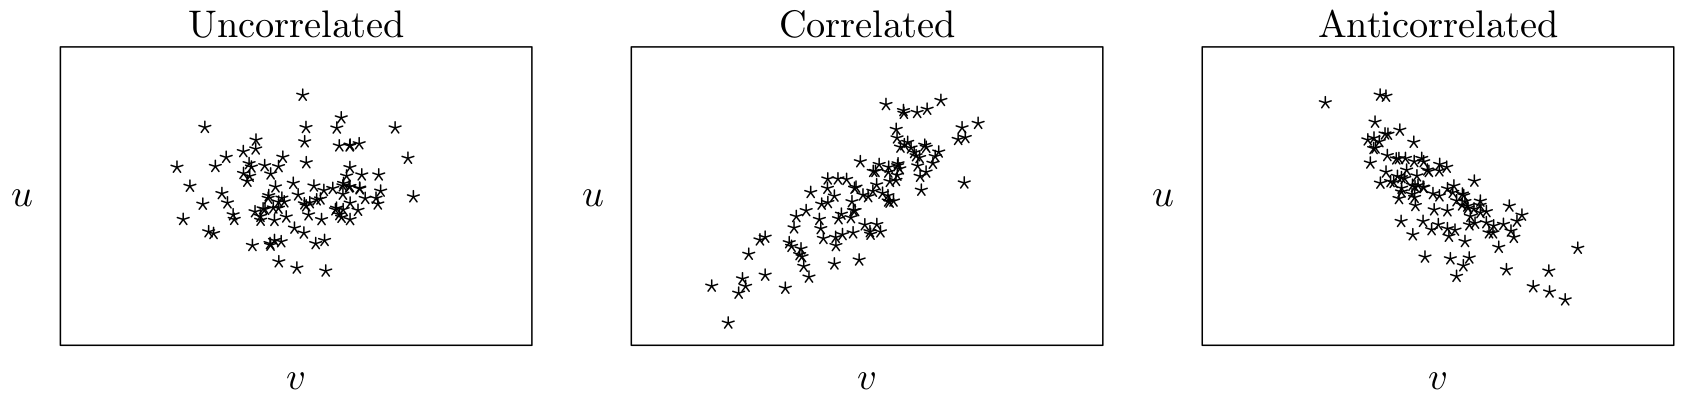
\includegraphics[width=0.95\textwidth]{figures/stats/corr_ex}
\caption{
Example distributions for
uncorrelated ($\rho \approx 0$),
correlated ($\rho \approx 1$),
and anticorrelated ($\rho \approx -1$)
variables $u$ and $v$ \cite{DougNotes}.
}
\label{fig:stats:corr_ex}
\end{figure}

The covariance matrix,

\begin{align}
  \mathbf{M} = \begin{pmatrix}
    \sigma_1^2   & \cov{1}{2} & \cov{1}{3} & \ldots \\
    \cov{1}{2}   & \sigma_2^2 & \cov{2}{3} & \ldots \\
    \cov{1}{3}   & \cov{2}{3} & \sigma_3^2 & \ldots \\
    \vdots       & \vdots     & \vdots     & \ddots
  \end{pmatrix}\,,
\end{align}

\noindent with elements $M_{ij} = \expval{\left(u_{i} - \bar{u}_{i}\right)\left(u_{j}-\bar{u}_{j}\right)}$
is the higher dimensional extension of the covariance.
We can visualize the covariance between variables with
Gaussian error ellipses given by the probability distribution

\begin{equation}\label{eq:stats:P_error_ellipse_k}
P\left(x_{1},x_{2},\ldots,x_{k}\right) = \frac{1}{(2\pi)^{k/2}}\frac{1}{\abs{\mathbf{M}}^{1/2}}\exp\left[-\frac{1}{2}\left(\mathbf{x}-\bm{\mu}\right)^{\transpose}\mathbf{M}\left(\mathbf{x}-\bm{\mu}\right)\right]\,,
\end{equation}

\noindent where the ellipse semi-axes are directed along the eigenvectors of $\mathbf{M}$.
In two dimensions it is easier to see the equation of the error ellipse itself:

\begin{equation}\label{eq:stats:P_error_ellipse_2}
\begin{split}
P\left(u,v\right) &= \frac{1}{2\pi\sigma_{u}\sigma_{v}}\frac{1}{\sqrt{1-\rho^{2}}}\exp\bigg\{-\frac{1}{2}\bigg[ \\
&\frac{1}{(1-\rho)^{2}}\left(\frac{\left(u-\bar{u}\right)^{2}}{\sigma_{u}^{2}}+\frac{\left(v-\bar{v}\right)^{2}}{\sigma_{v}^{2}}-\frac{2\rho \left(u-\bar{u}\right)\left(v-\bar{v}\right)}{\sigma_{u}\sigma_{v}}\right)\bigg]\bigg\}\,.
\end{split}
\end{equation}

%%%%%%%%%%%%%%%%%%%%%%%%%%%%%%%%%%%%%%%%%%%%%%%%%%%%%%%%
\subsection{Bias of a Predictor}
\label{additional:stats:bias}
% TODO

\begin{equation}\label{eq:stats:bias}
\bias{\hat{f}\left(x\right)} = \expval{\hat{f}\left(x\right)} - f\left(x\right)
\end{equation}

%%%%%%%%%%%%%%%%%%%%%%%%%%%%%%%%%%%%%%%%%%%%%%%%%%%%%%%%
\subsection{Principle Component Analysis (PCA)}
\label{additional:stats:PCA}
% TODO

%%%%%%%%%%%%%%%%%%%%%%%%%%%%%%%%%%%%%%%%%%%%%%%%%%%%%%%%
\subsection{Time Series Analysis}
\label{additional:stats:time_series_ana}
% TODO

%%%%%%%%%%%%%%%%%%%%%%%%%%%%%%%%%%%%%%%%%%%%%%%%%%%%%%%%
\subsection{Kalman Filters}
\label{additional:misc:kalman_filters}
% TODO

%%%%%%%%%%%%%%%%%%%%%%%%%%%%%%%%%%%%%%%%%%%%%%%%%%%%%%%%
\subsection{Markov Chains}
\label{additional:misc:markov_chains}
% TODO

%%%%%%%%%%%%%%%%%%%%%%%%%%%%%%%%%%%%%%%%%%%%%%%%%%%%%%%%
\subsection{Sampling from Probability Distributions}
\label{additional:misc:sampling_prob_dist}
Most programming languages have built-in functions to generate
pseudo-random numbers from common probability distributions,
such as the Poisson \cref{eq:stats:poisson:P} or Gaussian \cref{eq:stats:gaus:P} distributions.
However, in some cases we may wish to sample from an unsupported esoteric function.
In these situations we can turn to inverse transform sampling and rejection sampling,
to give just two examples from many possible computational methods,
to construct the desired distribution from an existing random number generator.

%%%%%%%%%%%%%%%%%%%%%%%%%%%%%%%%%%%%%%%%%%%%%%%%%%%%%%%%
\subsubsection{Inverse Transform Sampling}
\label{additional:misc:sampling_prob_dist:inverse}
% https://www.youtube.com/watch?v=9ixzzPQWuAY
If we know the explicit form of the target probability density function (PDF), $X = P\left(x\right)$,
can integrate it to find the cumulative distribution function (CDF), $F_{X}\left(x\right) = \int_{-\infty}^{x} P\left(t\right) \, \dif t$,
and furthermore can invert the CDF\footnote{The inverse CDF
is known as the percent point function, \texttt{ppf},
in \href{https://docs.scipy.org/doc/scipy-0.14.0/reference/stats.html}{\scipy}.}, $F^{-1}_{X}\left(u\right)$ for $0 \leq u \leq 1$,
we can explicitly transform the uniform distribution $U\left(x\right)$ into $P\left(x\right)$ as:

\begin{equation}\label{eq:stats:sampling_prob_dist:inverse}
F^{-1}_{X}\left(U\right) = P\left(x\right) = X\,.
\end{equation}

To prove the method, assuming that $F^{-1}_{X}$ exists, we can do:

\begin{subequations}\label{eq:stats:sampling_prob_dist:inverse_proof}
\begin{align}
P\left(F^{-1}_{X}\left(U\right) \leq x\right) &= P\left(U \leq F_{X}\left(x\right) \right) \label{eq:stats:sampling_prob_dist:inverse_proof:inverse} \\
&= F_{X}\left(x\right)\,,\label{eq:stats:sampling_prob_dist:inverse_proof:def} \\
P\left(U \leq y\right) &= y\,, \label{eq:stats:sampling_prob_dist:inverse_proof:U}
\end{align}
\end{subequations}

\noindent where in \cref{eq:stats:sampling_prob_dist:inverse_proof:inverse} we have applied $F$ to both sides of the inner inequality,
and in \cref{eq:stats:sampling_prob_dist:inverse_proof:def} we have used the definition of the uniform distribution \cref{eq:stats:sampling_prob_dist:inverse_proof:U}.
As $P\left(F^{-1}_{X}\left(U\right) \leq x\right) = F_{X}\left(x\right) = P\left(X \leq x\right)$
we can compare terms and see \cref{eq:stats:sampling_prob_dist:inverse}.

The inverse sampling method can be seen graphically \cref{fig:stats:sampling_prob_dist:inverse} being used to generate the normal distribution.

%\begin{figure}
%\centering
%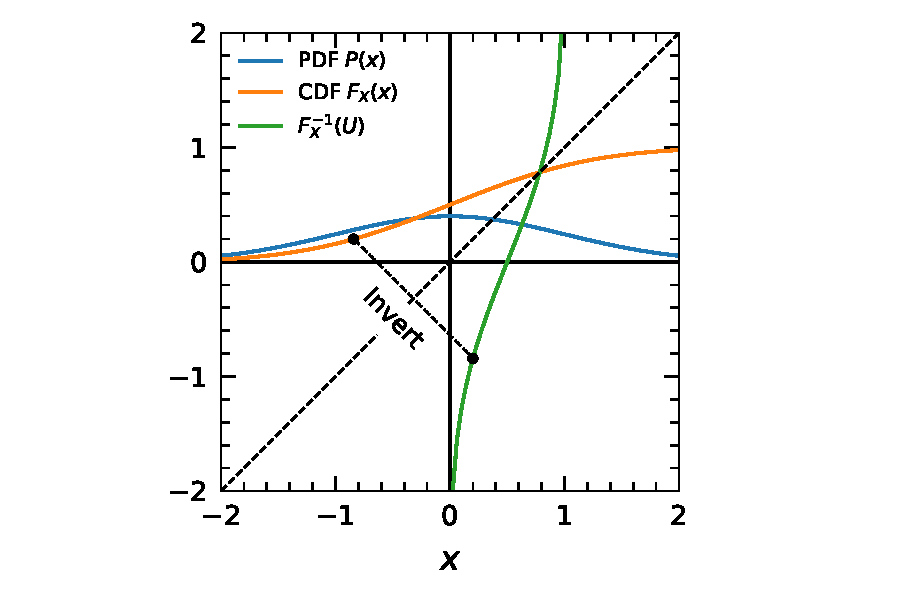
\includegraphics[width=0.7\textwidth]{figures/stats/inverse_transform_sampling_normal_dist}
%\caption{
%Example application of the inverse sampling method to generate the normal distribution, adapted from \href{https://en.wikipedia.org/wiki/File:Inverse_transform_sampling.png}{Olivier Ricou}.
%}
%\label{fig:stats:sampling_prob_dist:inverse}
%\end{figure}

%%%%%%%%%%%%%%%%%%%%%%%%%%%%%%%%%%%%%%%%%%%%%%%%%%%%%%%%
\subsubsection{Rejection Sampling}
\label{additional:misc:sampling_prob_dist:reject}
% https://www.youtube.com/watch?v=OXDqjdVVePY

While inverse transform sampling is a computationally efficient method
its assumptions will not be met by all interesting PDFs,
in particular if we do not have an explicit, invertible CDF.
In these cases we can turn to rejection sampling instead,
which can handle more general PDFs at the cost of a lower computational efficiency.

In rejection sampling, we assume we know the PDF of the random variable to be sampled from,
up to a normalization constant $A$ \cref{eq:stats:sampling_prob_dist:reject:X}.
We then choose a different PDF, $g\left(x\right)$ which is easy for us to sample from.
Any $g\left(x\right)$ covering the range of $x$ will do,
but the method is more efficient the closer we can get $g\left(x\right)$ to match $f\left(x\right)$.
$g\left(x\right)$ is then scaled by a known constant $M$
such that it is always larger than $f\left(x\right)$ \cref{eq:stats:sampling_prob_dist:reject:f_condition}
as illustrated in \cref{fig:stats:sampling_prob_dist:reject}.
Finally, we sample random $x$ values from $g\left(x\right)$ and accept them with probability \cref{eq:stats:sampling_prob_dist:reject:P_accept}.
The accepted $x$ values will have the same distribution as $X$.

\begin{subequations}\label{eq:stats:sampling_prob_dist:reject}
\begin{align}
X = P\left(x\right) &= \frac{1}{A} f\left(x\right), \label{eq:stats:sampling_prob_dist:reject:X} \\
\forall x, \quad f\left(x\right) & \leq M g\left(x\right), \label{eq:stats:sampling_prob_dist:reject:f_condition} \\
P\left(\text{Accept} \mid x\right) &= \frac{f\left(x\right)}{M g\left(x\right)}\,. \label{eq:stats:sampling_prob_dist:reject:P_accept}
\end{align}
\end{subequations}

\begin{figure}[H]
  \centering
  \savebox{\largestimage}{
    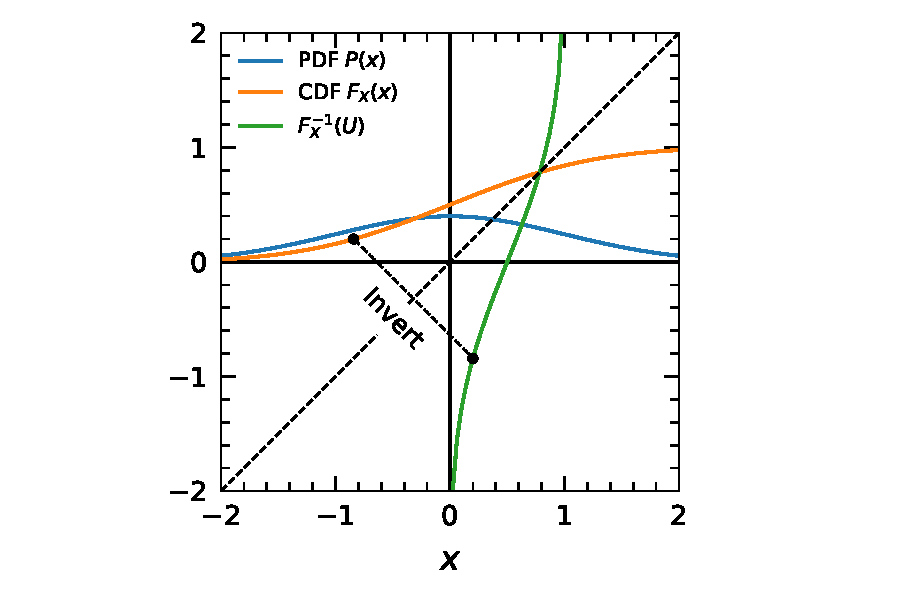
\includegraphics[width=0.47\textwidth,trim={3.0cm 0.5cm 3.0cm 0.1cm},clip]{figures/stats/inverse_transform_sampling_normal_dist}% trim={<left> <lower> <right> <upper>}
  }% Store largest image in a box

  \begin{subfigure}[b]{0.48\textwidth}\centering
    \usebox{\largestimage}
    \vspace{0.01cm}
  \caption{Inverse Sampling}
  \label{fig:stats:sampling_prob_dist:inverse}
  \end{subfigure}
  ~
  \begin{subfigure}[b]{\wd\largestimage}\centering
    \raisebox{\dimexpr.5\ht\largestimage-.5\height}{% Adjust vertical height of smaller image
      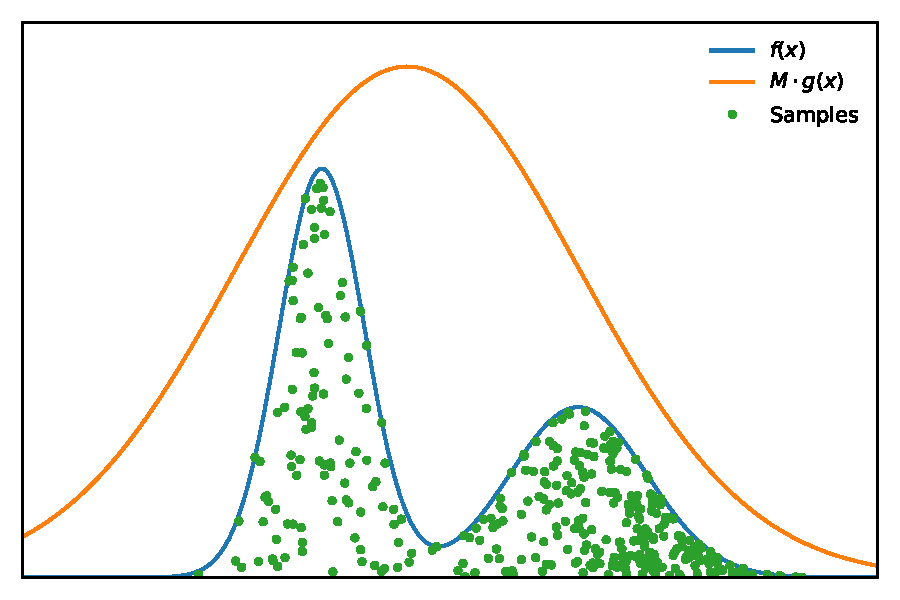
\includegraphics[width=\textwidth]{figures/stats/rejection_sampling}}
  \caption{Rejection Sampling}
  \label{fig:stats:sampling_prob_dist:reject}
  \end{subfigure}
\caption{
Illustrations of the inverse sampling and rejection sampling methods, adapted from \href{https://en.wikipedia.org/wiki/File:Inverse_transform_sampling.png}{Olivier Ricou} and \href{https://www.data-blogger.com/2016/01/24/the-mathematics-behind-rejection-sampling/}{Kevin Jacobs}.
  \label{fig:stats:sampling_prob_distr}
}
\end{figure}

For a proof of why the rejection sampling method works see \cref{eq:stats:sampling_prob_dist:reject:proof} below
which hinges on Bayes' Theorem from \cref{stats:Bayes} in \cref{eq:stats:sampling_prob_dist:reject:proof:x_given_Accept}
along with other basic definitions from probability theory.

\begin{subequations}\label{eq:stats:sampling_prob_dist:reject:proof}
\begin{align}
P\left(x \mid \text{Accept}\right) &= \frac{P\left(\text{Accept} \mid x\right) P\left(x\right)}{P\left(\text{Accept}\right)} = \frac{1}{P\left(\text{Accept}\right)} \frac{f\left(x\right)}{M \cancel{g\left(x\right)}} \cancel{g\left(x\right)}, \label{eq:stats:sampling_prob_dist:reject:proof:x_given_Accept} \\
P\left(\text{Accept}\right) &= \int_{-\infty}^{\infty} P\left(\text{Accept} \mid x\right) g\left(x\right) \, \dif x \label{eq:stats:sampling_prob_dist:reject:proof:P_Accept1} \\
&= \int_{-\infty}^{\infty} \frac{f\left(x\right)}{M g\left(x\right)} g\left(x\right) \, \dif x = \frac{1}{M} \int_{-\infty}^{\infty} f\left(x\right) \, \dif x = \frac{A}{M}, \label{eq:stats:sampling_prob_dist:reject:proof:P_Accept2} \\
\implies P\left(x \mid \text{Accept}\right) &= \frac{f\left(x\right)/M}{A/M} = \frac{1}{A} f\left(x\right) = P\left(x\right) = X. \label{eq:stats:sampling_prob_dist:reject:proof:conclusion}
\end{align}
\end{subequations}

%%%%%%%%%%%%%%%%%%%%%%%%%%%%%%%%%%%%%%%%%%%%%%%%%%%%%%%%
%%%%%%%%%%%%%%%%%%%%%%%%%%%%%%%%%%%%%%%%%%%%%%%%%%%%%%%%
\section{Regression}
\label{additional:Regression}

%%%%%%%%%%%%%%%%%%%%%%%%%%%%%%%%%%%%%%%%%%%%%%%%%%%%%%%%
\subsection{Gaussian Process Regression (Kriging)}
\label{additional:Regression:kriging}
% TODO

%%%%%%%%%%%%%%%%%%%%%%%%%%%%%%%%%%%%%%%%%%%%%%%%%%%%%%%%
\subsection{Principal Component Regression (PCR)}
\label{additional:Regression:PCR}
% TODO

%%%%%%%%%%%%%%%%%%%%%%%%%%%%%%%%%%%%%%%%%%%%%%%%%%%%%%%%
\subsection{Generalized Linear Models (GLM)}
\label{additional:Regression:GLM}
% TODO

%%%%%%%%%%%%%%%%%%%%%%%%%%%%%%%%%%%%%%%%%%%%%%%%%%%%%%%%
\subsection{Poisson Regression}
\label{additional:Regression:poisson}
% TODO


%%%%%%%%%%%%%%%%%%%%%%%%%%%%%%%%%%%%%%%%%%%%%%%%%%%%%%%%
%%%%%%%%%%%%%%%%%%%%%%%%%%%%%%%%%%%%%%%%%%%%%%%%%%%%%%%%
\section{Survival Analysis}
\label{additional:Survival}

Survival analysis is a subfield of statistics which examines problems involving the timing of events
such as death, component failure, or exiting a line of therapy after an adverse effect, in a population of subjects under study.
Using the appropriate models, quantities such as the lifetime, or failure rate, of a subject
can be estimated, as well as their dependence on other independent variables.
A variety of common models are available,
each with their own assumptions, capabilities, and limitations,
which make them best suited for certain applications.

%%%%%%%%%%%%%%%%%%%%%%%%%%%%%%%%%%%%%%%%%%%%%%%%%%%%%%%%
\subsection{Nomenclature}
\label{additional:Survival:Nomenclature}

\begin{symbollist}
	\item[Event] The event of interest in a study, \eg death, component failure\ldots
	\item[$t$] Time from the start of observation to an event, the conclusion of the study, or the withdrawal of a subject.
	\item[$T$] Time that an event occurred.
	\item[$x$] Independent variable(s) under consideration.
	\item[Censoring] Right\footnote{Left censored subjects enter the study after the event of interest has already occurred at an unknown $t < 0$.} censored subjects have no events during the observation period, either due to early withdrawal or the conclusion of the study. The true lifetime of these subjects is unavailable for analysis, \ie they have been censored.
	\item[$S\left(t\right)$] The survival function $S\left(t\right)$ is the probability that a subject survives longer than $t$, \ie $S\left(t\right) = P\left(T > t\right)$.
	\item[$F\left(t\right)$] The lifetime distribution function $F\left(t\right)$ is the complement of the survival function, \ie $F\left(t\right) = 1 - S\left(t\right) = P\left(T \leq t\right)$.
	\item[$f\left(t\right)$] The event density function $f\left(t\right)$ is the time derivative of the lifetime distribution function $F\left(t\right)$, $f\left(t\right) = \frac{dF}{dt} = -\frac{dS}{dt}$, if it exists.
	\item[$\lambda\left(t\right)$] The hazard function $\lambda\left(t\right)$ is the event rate at $t$ conditional on survival to time $t$, \ie $T > t$, see \cref{eq:Survival:hazard_def}. Any $\lambda\left(t\right)$ can be a hazard function, provided it satisfies \cref{eq:Survival:hazard_cond}.
	\item[$\Lambda\left(t\right)$] The cumulative hazard function $\Lambda\left(t\right)$ is the integral of $\lambda\left(t\right)$ with respect to time \cref{eq:Survival:cum_hazard:def}. Also see the relations in \cref{eq:Survival:cum_hazard:to_lambda,eq:Survival:cum_hazard:to_S}.
	\item[HR] The hazard ratio (HR) compares the hazards of two subsets of subjects partitioned by $x$ at time $t$, $\text{HR} = \lambda\left(x = 1\right) / \lambda\left(x=0\right)$.
\end{symbollist}

\begin{subequations}\label{eq:Survival:hazard_def}
\begin{align}
\lambda\left(t\right) dt &= P\left(T \leq t + dt \mid T > t\right),\,\text{as} \,\, dt \to 0 \label{eq:Survival:hazard_def:a} \\
\lambda\left(t\right) &= \lim_{dt \to 0} \frac{P\left(T \leq t + dt \cap T > t\right)}{P\left(T > t\right)\,dt} \label{eq:Survival:hazard_def:b} \\
&= \frac{1}{S\left(t\right)} \lim_{dt \to 0} \frac{P\left(t < T \leq t + dt\right)}{dt} \label{eq:Survival:hazard_def:c} \\
&= \frac{1}{S\left(t\right)} \lim_{dt \to 0} \frac{F\left(t + dt\right) - F\left(t\right)}{dt} \label{eq:Survival:hazard_def:d} \\
&= \frac{f\left(t\right)}{S\left(t\right)} = -\frac{1}{S} \frac{dS}{dt} \label{eq:Survival:hazard_def:e}
\end{align}
\end{subequations}

\begin{subequations}\label{eq:Survival:hazard_cond}
\begin{gather}
\forall t \geq 0, \, \lambda\left(t\right) \geq 0 \label{eq:Survival:hazard_cond:a} \\
\int_{0}^{\infty} \lambda\left(t\right) \, \dif t = \infty \label{eq:Survival:hazard_cond:b}
\end{gather}
\end{subequations}

\begin{subequations}\label{eq:Survival:cum_hazard}
\begin{gather}
\Lambda\left(t\right) = \int_{0}^{t} \lambda\left(u\right) \, \dif u = - \ln\left(S\left(t\right)\right) \label{eq:Survival:cum_hazard:def} \\
\lambda\left(t\right) = \frac{d\Lambda}{dt} = -\frac{1}{S} \frac{dS}{dt} \label{eq:Survival:cum_hazard:to_lambda} \\
S\left(t\right) = \exp\left(-\Lambda\left(t\right)\right) \label{eq:Survival:cum_hazard:to_S}
\end{gather}
\end{subequations}

%%%%%%%%%%%%%%%%%%%%%%%%%%%%%%%%%%%%%%%%%%%%%%%%%%%%%%%%
\subsection{Kaplan-Meier Model}
\label{additional:Survival:km}

The Kaplan-Meier model \cite{km} $\hat{S}_{\text{KM}}\left(t\right)$ is a non-parametric
estimate of $S\left(t\right)$ computed from empirical data.

\begin{equation}\label{eq:Survival:km}
\hat{S}_{\text{KM}}\left(t\right) = \prod_{i:\,t_{i} < t} \left(1 - \frac{d_{i}}{n_{i}}\right)
\end{equation}

\noindent Here the product is over all times $t_{i}$ at which $d_{i}$ events occurred,
and $n_{i}$ is the number of subjects still under study at $t_{i}$,
\ie subjects who have not had an event or been censured.
Due to its construction, $\hat{S}_{\text{KM}}\left(t\right)$ remains steady
between $t_{i}$ but drops vertically at each data point.
Therefore the derivative does not exist and we can not estimate $f\left(t\right)$ or $\lambda\left(t\right)$.
See \cref{fig:stanford_km:km} for one example of a Kaplan-Meier curve.

We can apply the Kaplan-Meier estimator to different subsets of subjects partitioned by a categorical variable $x$
in order to understand the dependence of $S\left(t\right)$ on $x$.
Note that $x$ can not be a continuous variable, and must be binned to integer classes if that is the case.

%%%%%%%%%%%%%%%%%%%%%%%%%%%%%%%%%%%%%%%%%%%%%%%%%%%%%%%%
\subsection{Exponential Model}
\label{additional:Survival:exp}

The exponential model is a parametric estimate of $S\left(t\right)$
valid when the hazard is expected to be constant with respect to $t$.
In nuclear physics\footnote{$\frac{dN}{dt} = -\lambda N$, $N\left(t\right) = N_{0} e^{-\lambda t}$, half-life $t_{1/2} = \ln\left(2\right) / \lambda = \tau \ln\left(2\right)$, where $\tau$ is the time constant.} $\lambda\left(t\right) = \lambda$
decays per unit time really is a constant.
However, in most situations $\lambda = c$ is unrealistic over longer time scales,
as illustrated in \cref{additional:Survival:additional:bathtub}.
The exponential model can accommodate both categorical and continuous $x$ independent variables.

The survival function for the exponential model is simply

\begin{equation}\label{eq:Survival:exp}
\hat{S}_{\text{Exp}}\left(t\right) = e^{-\lambda t}
\end{equation}

\noindent where the hazard can be expanded in terms of $\mathbf{x}$, $\bm{\beta}$ as in a regression analysis:

\begin{equation}\label{eq:Survival:exp_lambda}
\begin{aligned}
\lambda\left(x\right) &= \exp\left(\beta_{0} + \sum_{j=1}^{n}\, \beta_{j} x_{j}\right) \\
\log\left(\lambda\right) &= \mathbf{x} \bm{\beta}
\end{aligned}
\end{equation}

\noindent Here we are making the {\em proportional hazards assumption},
\ie the differences in $\lambda$ between subgroups in $x_{j}$
are proportional\footnote{Really $\log\left(\lambda\right) \propto \beta$.} to $\beta_{j}$
and constant over $t$.
To find the best estimate of $\hat{\bm{\beta}}$,
$\lambda$ is used to derive a likelihood function which is
then optimized\footnote{The exact details of this optimization are handled by common software libraries and are omitted here. Similar approaches are also used to fit the later Weibull and Cox proportional-hazards models.}.

The hazard ratio for $x_{j}$ is:

\begin{equation}\label{eq:Survival:exp_HR}
\begin{aligned}
\text{HR}_{\text{Exp}} &= e^{\ldots+\beta_{j} 1+\ldots} / e^{\ldots+\beta_{j} 0+\ldots} \\
&= e^{\beta_{j}}
\end{aligned}
\end{equation}

\subsubsection{Weibull Model}
\label{additional:Survival:weibull}

The Weibull model expands on the standard exponential model
by introducing a shape parameter $k$ to adjust the time dependence of the hazard:

\begin{equation}\label{eq:Survival:weibull}
\begin{aligned}
\hat{S}_{\text{Weibull}}\left(t\right) &= e^{-\lambda_{\text{Weibull}} t} \\
\lambda_{\text{Weibull}} &= \exp\left(\beta_{0} t^{k} + \sum_{j=1}^{n}\, \beta_{j} x_{j}\right) \\
\text{HR}_{\text{Weibull}} &= e^{\beta_{j}}
\end{aligned}
\end{equation}

\noindent Here $\beta_{0}$ is the scale parameter of the hazard with respect to $t$,
while the other $\beta_{j}$ are scale parameters for the independent $x_{j}$.
For $k<0$ ($k>0$) the hazard monotonically decreases (increases) over time,
while $k=0$ returns the exponential model.
This allows phenomena such as burn in and compounding component failures to be modeled.
Numerous parameterizations and expansions of the Weibull model are available,
however they all share the property that
$\lambda = \exp\left(\beta_{0} f\left(t\right) + \sum_{j=1}^{n}\, \beta_{j} x_{j}\right)$
where $f\left(t\right)$ is a {\em known}, almost always monotonic, function of $t$.

%%%%%%%%%%%%%%%%%%%%%%%%%%%%%%%%%%%%%%%%%%%%%%%%%%%%%%%%
\subsection{Cox Proportional-Hazards Model}
\label{additional:Survival:cox}

The Cox proportional-hazards model \cite{cox} is a
semiparametric\footnote{Semiparametric as $\lambda_{0}\left(t\right)$ is unspecified, but $\bm{\beta}$ are still parameters of $\lambda$.} model
which further expands on the Weibull model by allowing
the time dependence of $\lambda$ to be an unknown function.
As the name suggests, the proportional hazards assumption is retained
allowing us to compute useful HR values
without even knowing $\lambda\left(t\right)$, or $S\left(t\right)$.

In the Cox model we assume the hazard has the form of

\begin{equation}\label{eq:Survival:cox_lambda}
\lambda_{\text{Cox}} = \lambda_{0}\left(t\right) \exp\left(\sum_{j=1}^{n}\, \beta_{j} x_{j}\right)
\end{equation}

\noindent where $\lambda_{0}\left(t\right)$ is the baseline hazard, an unspecified function of $t$.
When computing hazard ratios $\lambda_{0}\left(t\right)$ then drops out:

\begin{equation}\label{eq:Survival:cox_HR}
\text{HR}_{\text{Exp}} = e^{\beta_{j}}
\end{equation}

%%%%%%%%%%%%%%%%%%%%%%%%%%%%%%%%%%%%%%%%%%%%%%%%%%%%%%%%
\subsection{Method Comparison}
\label{additional:Survival:comp}

\begin{table}[H]
\centering
\begin{tabular}{l|l|l}
\multicolumn{1}{c|}{Kaplan-Meier} & \multicolumn{1}{c|}{Exponential / Weibull} & \multicolumn{1}{c}{Cox} \\
\cline{1-3}
\begin{tabular}[c]{p{0.3\textwidth}}
Pro
\begin{itemize}
	\item Simple to compute and understand
	\item Can estimate $S$
\end{itemize}
\\
Con
\begin{itemize}
	\item No functional form
	\item Can \textbf{not} estimate HR
	\item Only can handle a few categorical $x$
\end{itemize}
\end{tabular}

&

\begin{tabular}[c]{p{0.3\textwidth}}
Pro
\begin{itemize}
	\item Can estimate $S$ and HR
\end{itemize}
\\
Con
\begin{itemize}
	\item $\lambda\left(t\right) = c$ can be unrealistic
	\item Weibull: $\lambda = f\left(t\right)$ of a known form
\end{itemize}
\end{tabular}

&

\begin{tabular}[c]{p{0.3\textwidth}}
Pro
\begin{itemize}
	\item $\lambda$ can be an unknown function of $t$
	\item Can estimate HR
\end{itemize}
\\
Con
\begin{itemize}
	\item Can \textbf{not} estimate $S$
\end{itemize}
\end{tabular}

\\
\end{tabular}
\end{table}

%%%%%%%%%%%%%%%%%%%%%%%%%%%%%%%%%%%%%%%%%%%%%%%%%%%%%%%%
\subsection{Model Assumptions}
\label{additional:Survival:assumptions}

\begin{enumerate}[noitemsep]
\item Any censoring is non-informative, \ie censoring is uncorrelated with the probabilities of different event outcomes.\label{item:Survival:assumptions:censoring}
\item Survival times $t$ are uncorrelated across subjects.\label{item:Survival:assumptions:t_uncorr}
\item $\mathbf{x}$ is constant over time, per subject.\label{item:Survival:assumptions:X_constant}
\item Hazards are proportional, \ie hazard ratios are constant over time.\label{item:Survival:assumptions:prop_hazard}
\item $\log\left(\lambda\right)$ is linear with respect to the numerical $x_{j}$ independent variables.\label{item:Survival:assumptions:X_linearity}
\end{enumerate}

\cref{item:Survival:assumptions:censoring,item:Survival:assumptions:t_uncorr,item:Survival:assumptions:X_constant}
are assumptions for all survival models, while
\cref{item:Survival:assumptions:prop_hazard,item:Survival:assumptions:X_linearity}
apply to the exponential, Weibull and Cox models.

\subsubsection{Tests and Corrections}
\label{additional:Survival:assumptions:tests_and_corrections}

\begin{itemize}[noitemsep]
\item[\cref{item:Survival:assumptions:censoring}.] Exploratory data analysis to detect differences in $\mathbf{x}$ distributions between censored and non-censored subjects. If violated, better input data is needed, redesign study.

\item[\cref{item:Survival:assumptions:t_uncorr}.] Exploratory data analysis, study design question. If violated, redesign study.

\item[\cref{item:Survival:assumptions:X_constant}.] Exploratory data analysis, study design question. If unavoidable, can try a more complex time dependent covariate model.

\item[\cref{item:Survival:assumptions:prop_hazard}.] Check with a Schoenfeld test or complementary log-log plot. If violated, stratify problematic $x_{j}$ variables into separate models, or use more complex models with time dependent $\beta$ coefficients.

\item[\cref{item:Survival:assumptions:X_linearity}.] Check the appropriate residual plot. If violated, try to linearize the offending numerical $x_{j}$ with a transformation or bin to a categorical variable.
\end{itemize}

\subsubsection{Schoenfeld Test}
\label{additional:Survival:assumptions:schoenfeld}

Schoenfeld residuals are similar in concept to normal residuals in regression analyses,
but instead of looking at the difference between the true and estimated values of $y$,
$\hat{\bm{\epsilon}} = \mathbf{y} - \mathbf{X} \hat{\bm{\beta}}$,
we look at the difference in $\bm{\beta}$ and $\hat{\bm{\beta}}$ for a particular $y$ value.
In this way, Schoenfeld residuals represent the difference in the
coefficient $\beta_{j}$ fit from all data points, and a single point.
To validate the proportional hazards assumption
the Schoenfeld residuals \cite{schoenfeld} must not change over time.
An example Schoenfeld residual plot is provided in
\cref{fig:cox:schoenfeld_residuals}.
Besides graphically looking at the residuals,
we can use $\chi^{2}$-tests to compute {\pvalue}s
to test the null hypothesis, \ie the Schoenfeld residuals and time are independent.
In this case, the proportional hazards assumption is supported
if we find large, non-significant {\pvalue}s.

\subsubsection{Complementary Log-Log Plot}
\label{additional:Survival:assumptions:cloglog}

For categorical variables we can look at the
complementary log-log plot
of $\log\left(-\log\left(S\left(t\right)\right)\right)$ versus $\log\left(t\right)$.
An example complementary log-log plot is provided in \cref{fig:stanford_cloglog}.
If the different categories have parallel curves
the proportional hazards assumption is
valid for the variable in question.

%%%%%%%%%%%%%%%%%%%%%%%%%%%%%%%%%%%%%%%%%%%%%%%%%%%%%%%%
\subsection{Additional Concepts}
\label{additional:Survival:additional}

\subsubsection{Logrank Test}
\label{additional:Survival:additional:logrank}
% TODO comparing survival curves

\subsubsection{$G^{\rho}$ Test (survdiff)}
\label{additional:Survival:additional:survdiff}
% TODO comparing survival curves
TODO \texttt{survdiff}

\subsubsection{Concordance Statistic}
\label{additional:Survival:additional:concordance}
% TODO

\subsubsection{Relative Risk}
\label{additional:Survival:additional:RR}
% TODO relationship / differences from HR

\subsubsection{Odds Ratio}
\label{additional:Survival:additional:OR}
% TODO relationship / differences from HR

\subsubsection{Expected Future Lifetime}
\label{additional:Survival::additional:efl}

The expected future lifetime $\expval{T-t_{0}}$ is the
expected additional time of survival for a subject having already survived to $t_{0}$.
We can derive $\expval{T-t_{0}}$ \cref{eq:Survival:efl_der:efl}
from the probability of an event occurring between $t_{0}$ and $t_{0} + t$ \cref{eq:Survival:efl_der:P}
using the prior work of \cref{eq:Survival:hazard_def} and integration by parts:

\begin{subequations}\label{eq:Survival:efl_der}
\begin{gather}
P\left(T \leq t_{0} + t \mid T > t_{0}\right)
= \frac{F\left(t_{0} + t\right) - F\left(t_{0}\right)}{S\left(t_{0}\right)} \label{eq:Survival:efl_der:P} \\
\text{PDF}
= \frac{d}{dt} P\left(T \leq t_{0} + t \mid T > t_{0}\right)
= \frac{f\left(t_{0} + t\right)}{S\left(t_{0}\right)} \label{eq:Survival:efl_der:pdf} \\
\expval{T-t_{0}}
= \int_{0}^{\infty} t \, \text{PDF} \, \dif t
= \frac{1}{S\left(t_{0}\right)} \int_{0}^{\infty} S\left(t\right) \, \dif t \label{eq:Survival:efl_der:efl}
\end{gather}
\end{subequations}

\subsubsection{Bathtub Curve}
\label{additional:Survival:additional:bathtub}

In reliability engineering the hazard function of many components
can be estimated as a three part ``bathtub'' curve.
Initially the failure, \ie event, rate decreases as defective components fail early,
before reaching a constant plateau where failures are essentially random events.
As components wear out and reach the end of their useful lifetimes, the failure rate increases again.
Combining these three effects produces a bathtub-shaped curve, as seen in \cref{fig:bathtub_curve}.
We can model these situations with the Cox proportional-hazards model,
or a Weibull model with an appropriately shaped $\lambda\left(t\right)$.

\begin{figure}[H]
\centering
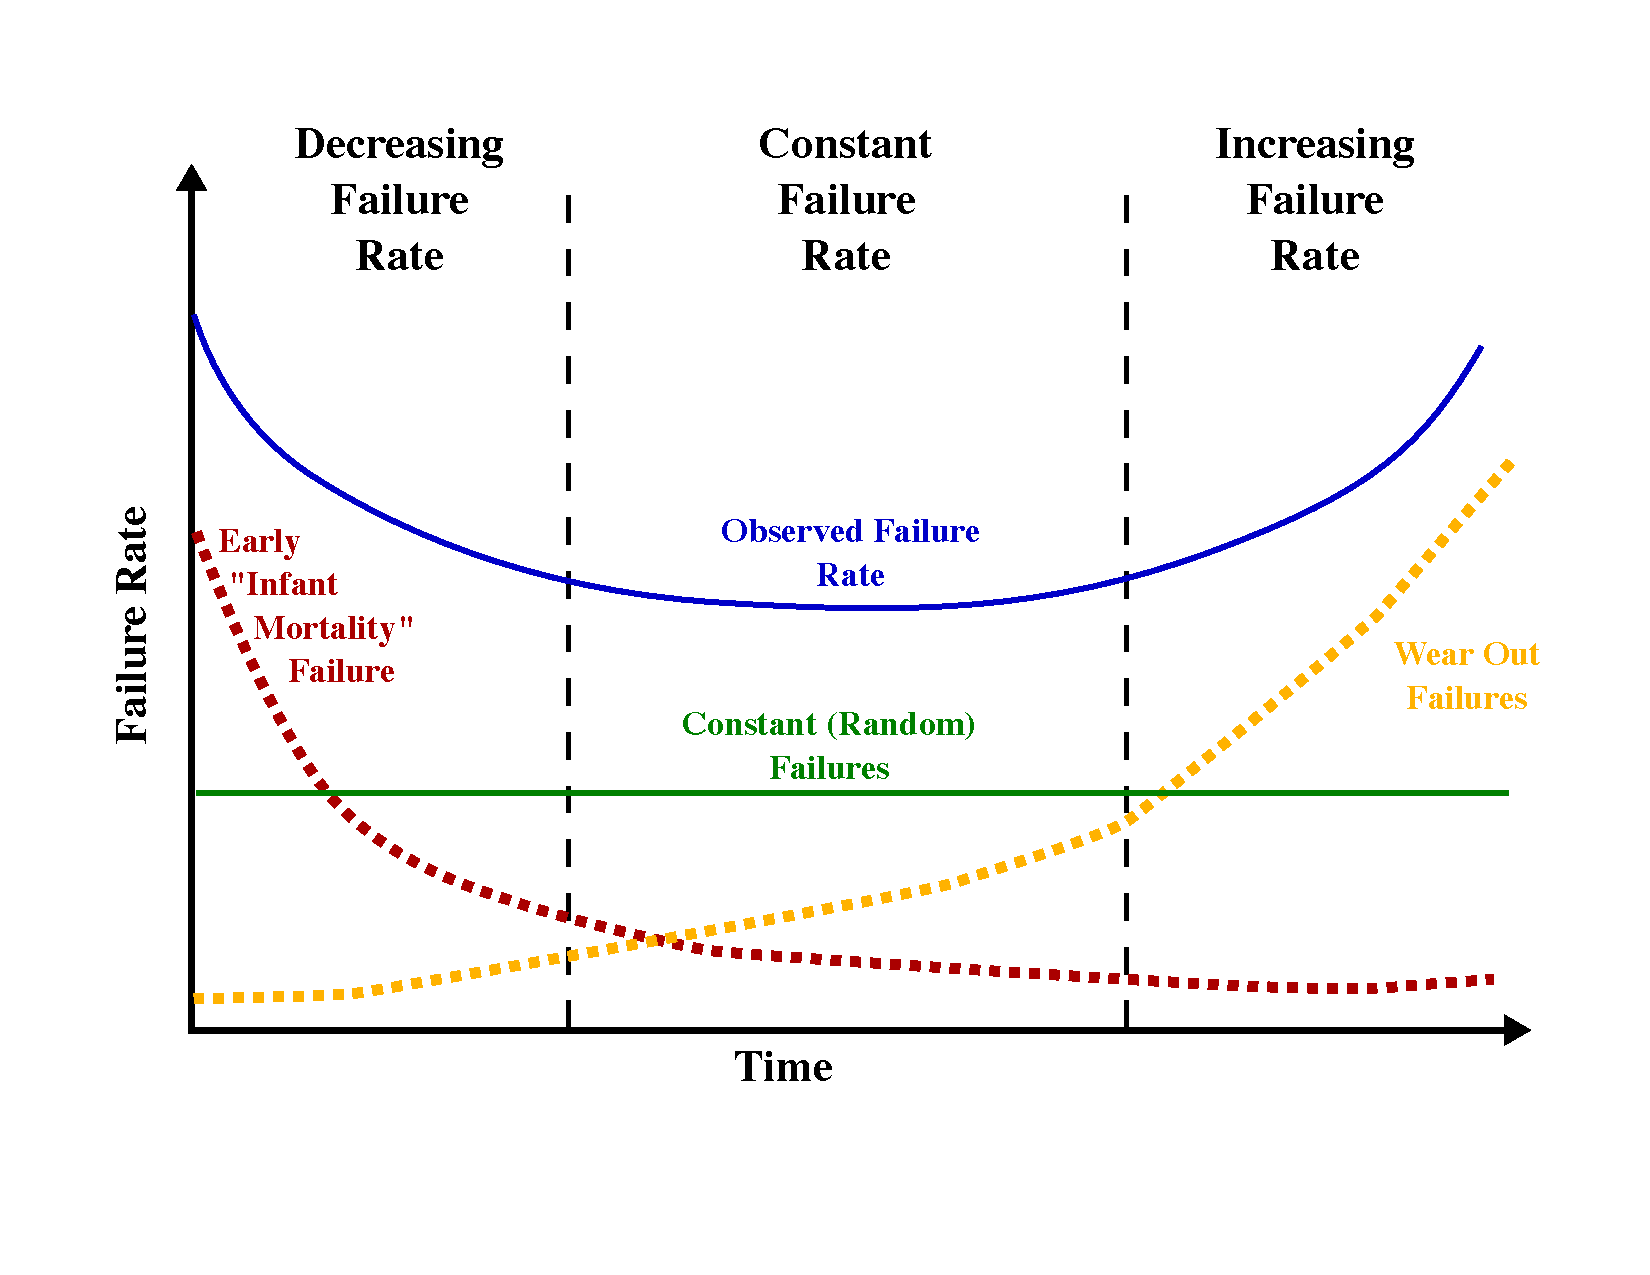
\includegraphics[width=0.7\textwidth]{figures/survival/bathtub_curve}
\vspace{0.2cm}
\caption{
Illustration of a bathtub curve hazard function, by \href{https://en.wikipedia.org/wiki/File:Bathtub_curve.svg}{Wyatts}.
}
\label{fig:bathtub_curve}
\end{figure}

%%%%%%%%%%%%%%%%%%%%%%%%%%%%%%%%%%%%%%%%%%%%%%%%%%%%%%%%
\subsection{Example \R Code}
\label{additional:Survival:Rcode}

% TODO link to code section from body section(s)

A simple example survival analysis in \R utilizing the built-in
\texttt{stanford2} Stanford heart transplant dataset is provided in this section.
The full code can also be found in
\href{https://github.com/mepland/data_science_notes/blob/main/sections/appendixes/additional/example_survival.R}{\texttt{example\_survival.R}}.
The status variable represents the event, death of a patient, as $\text{status}=1$,
and the censoring of a patient as $\text{status}=0$.
Three independent variables $x$ are available,
age in years,
age categories - under or over 40,
and the numeric T5 mismatch score between donor and recipient.

\begin{figure}[H]
\centering
  \begin{subfigure}[c]{0.48\textwidth}\centering
  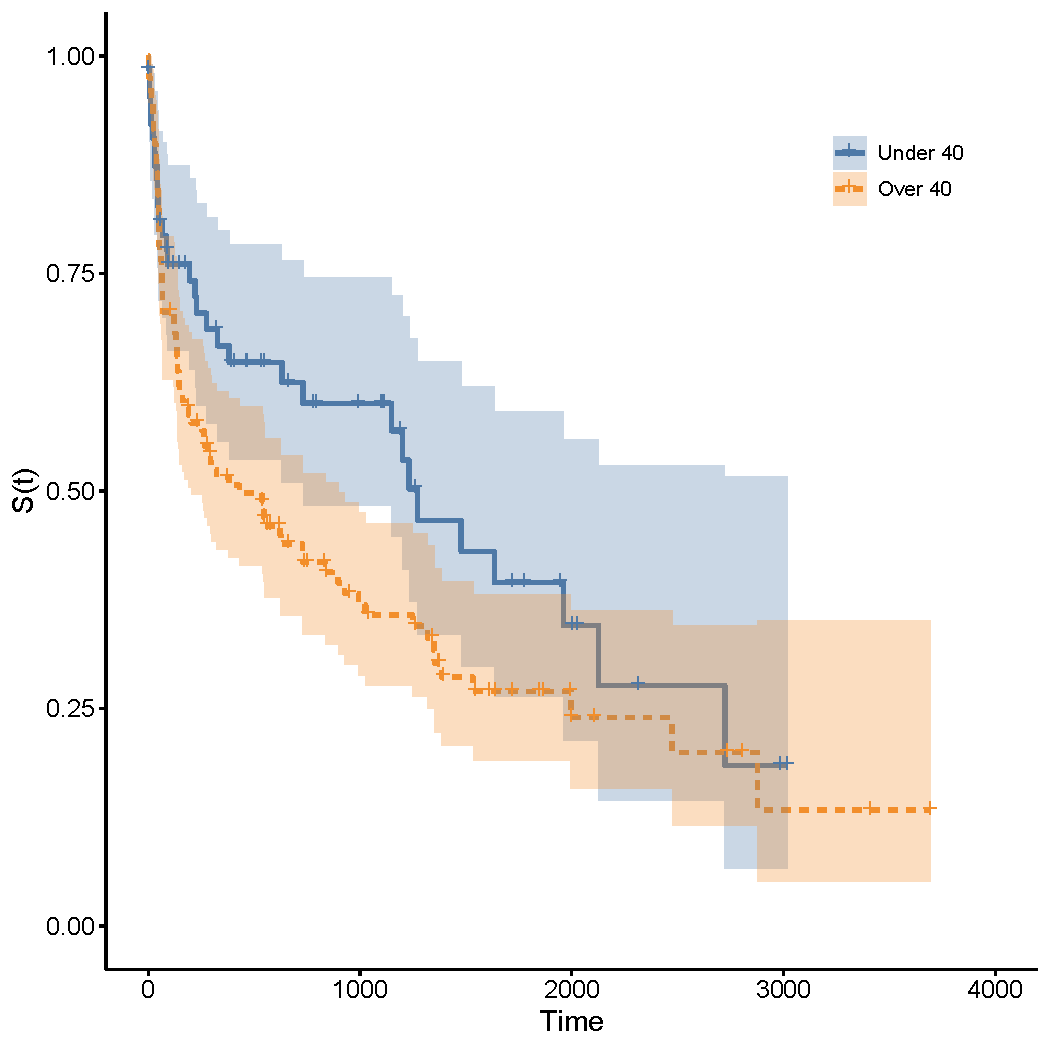
\includegraphics[width=\textwidth]{figures/survival/stanford_km}
  \caption{Kaplan-Meier}
  \label{fig:stanford_km:km}
  \end{subfigure}
  ~
  \begin{subfigure}[c]{0.48\textwidth}\centering
  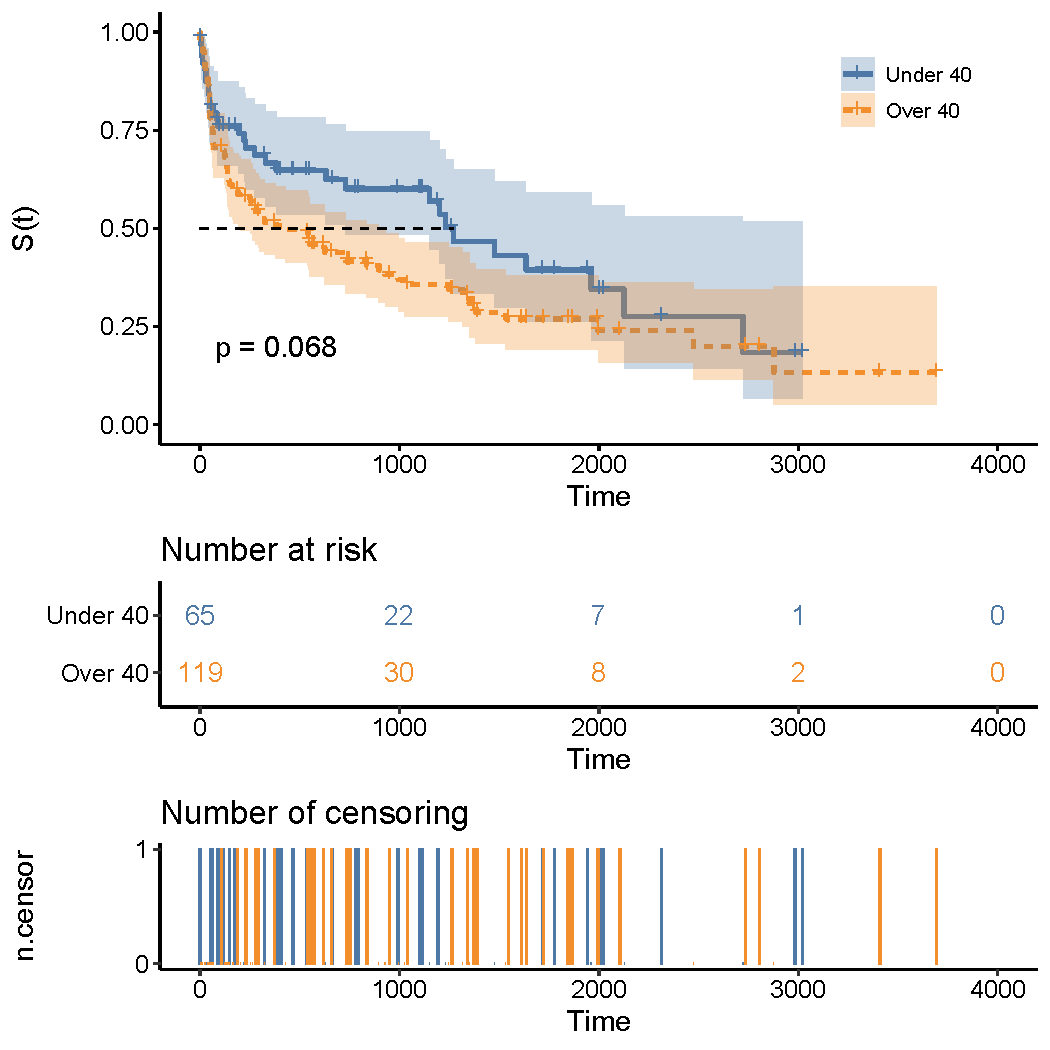
\includegraphics[width=\textwidth]{figures/survival/stanford_km_annotated}
  \caption{Annotated}
  \label{fig:stanford_km:annotated}
  \end{subfigure}
\caption{
Kaplan-Meier plot of the Stanford heart transplant dataset. Censored patients are displayed with marks.
The version on the right adds additional annotations, such as
subplots for patients at risk and censoring events,
the \pvalue from \texttt{survdiff}, and a median reference line.
}
\label{fig:stanford_km}
\end{figure}

\subsubsection{Initialization}
\label{additional:Survival:Rcode:init}

\begin{lstlisting}[language=R]
> install.packages(c("survival", "survminer"))
> library("survival")
> library("survminer")

> df <- stanford2
> df$agecat <- cut(df$age, breaks=c(0,40, Inf), labels=c('Under 40', 'Over 40'), right=FALSE)
> df <- df[with(df, order(time)),]

> df[1:5,c('time', 'status', 'age', 'agecat', 't5')]
    time status age   agecat   t5
21   0.5      1  41  Over 40 0.87
133  1.0      1  21 Under 40 0.47
184  1.0      0  27 Under 40   NA
16   1.0      1  54  Over 40 0.47
183  2.0      0  39 Under 40   NA
> summary(df[c('time', 'agecat', 't5')])
      time              agecat          t5
 Min.   :   0.50   Under 40: 65   Min.   :0.000
 1st Qu.:  64.75   Over 40 :119   1st Qu.:0.690
 Median : 351.00                  Median :1.040
 Mean   : 696.94                  Mean   :1.117
 3rd Qu.:1160.75                  3rd Qu.:1.460
 Max.   :3695.00                  Max.   :3.050
                                  NA's   :27
\end{lstlisting}

\subsubsection{Kaplan-Meier Model}
\label{additional:Survival:Rcode:km}

\begin{lstlisting}[language=R]
> km.model <- survfit(Surv(time, status) ~ agecat, data=df, type='kaplan-meier')
> summary(km.model)$table
                records n.max n.start events   *rmean *se(rmean) median 0.95LCL 0.95UCL
agecat=Under 40      65    65      65     32 1520.783   220.1031   1271     731      NA
agecat=Over 40      119   119     119     81 1123.229   143.3516    431     202     897

> survdiff(Surv(time, status) ~ agecat, data=df)
Call:
survdiff(formula = Surv(time, status) ~ agecat, data = df)

                  N Observed Expected (O-E)^2/E (O-E)^2/V
agecat=Under 40  65       32     41.3      2.10      3.32
agecat=Over 40  119       81     71.7      1.21      3.32

 Chisq= 3.3  on 1 degrees of freedom, p= 0.07

> pdf('~/stanford_km.pdf')
> ggsurvplot(km.model, xlab='Time', ylab='S(t)', size = 1, linetype = 'strata', palette=c('#4e79a7', '#f28e2b'), conf.int = TRUE, legend = c(0.85, 0.85), legend.y = 1, legend.title = '', legend.labs = c('Under 40', 'Over 40'))
> dev.off()

> pdf('~/stanford_km_annotated.pdf')
> ggsurvplot(km.model, xlab='Time', ylab='S(t)', size = 1, linetype = 'strata', palette=c('#4e79a7', '#f28e2b'), conf.int = TRUE, legend = c(0.85, 0.85), legend.y = 1, legend.title = '', legend.labs = c('Under 40', 'Over 40'),
pval = TRUE, # Add survdiff p-value
risk.table = TRUE, # Absolute number at risk
risk.table.y.text.col = FALSE, risk.table.col = "strata",
ncensor.plot = TRUE, # plot censored patients vs time
surv.median.line = "h", # add horizontal median
)
> dev.off()
\end{lstlisting}

\subsubsection{Cox Proportional-Hazards Model}
\label{additional:Survival:Rcode:cox}

\begin{lstlisting}[language=R]
> cox.model_age <- coxph(Surv(time, status) ~ age, data=df[!is.na(df$t5), ])
> summary(cox.model_age)
Call:
coxph(formula = Surv(time, status) ~ age, data = df[!is.na(df$t5),
    ])

  n= 157, number of events= 102

       coef exp(coef) se(coef)     z Pr(>|z|)
age 0.02990   1.03035  0.01136 2.633  0.00846 **
---
Signif. codes:  0 ‘***’ 0.001 ‘**’ 0.01 ‘*’ 0.05 ‘.’ 0.1 ‘ ’ 1

    exp(coef) exp(-coef) lower .95 upper .95
age      1.03     0.9705     1.008     1.054

Concordance= 0.595  (se = 0.034 )
Likelihood ratio test= 7.62  on 1 df,   p=0.006
Wald test            = 6.93  on 1 df,   p=0.008
Score (logrank) test = 7.01  on 1 df,   p=0.008

> cox.model_age_t5 <- coxph(Surv(time, status) ~ age + t5, data=df[!is.na(df$t5), ])
> summary(cox.model_age_t5)
Call:
coxph(formula = Surv(time, status) ~ age + t5, data = df[!is.na(df$t5),
    ])

  n= 157, number of events= 102

       coef exp(coef) se(coef)     z Pr(>|z|)
age 0.02961   1.03006  0.01136 2.608  0.00911 **
t5  0.17041   1.18579  0.18326 0.930  0.35243
---
Signif. codes:  0 ‘***’ 0.001 ‘**’ 0.01 ‘*’ 0.05 ‘.’ 0.1 ‘ ’ 1

    exp(coef) exp(-coef) lower .95 upper .95
age     1.030     0.9708     1.007     1.053
t5      1.186     0.8433     0.828     1.698

Concordance= 0.59  (se = 0.034 )
Likelihood ratio test= 8.47  on 2 df,   p=0.01
Wald test            = 7.81  on 2 df,   p=0.02
Score (logrank) test = 7.87  on 2 df,   p=0.02

> anova(cox.model_age, cox.model_age_t5, test='LRT')
Analysis of Deviance Table
 Cox model: response is  Surv(time, status)
 Model 1: ~ age
 Model 2: ~ age + t5
   loglik Chisq Df P(>|Chi|)
1 -447.29
2 -446.86 0.851  1    0.3563
\end{lstlisting}

\subsubsection{Checking Assumptions}
\label{additional:Survival:Rcode:assumptions}

\begin{lstlisting}[language=R]
# proportional hazards
> cox.model_age.ph <- cox.zph(cox.model_age)
> cox.model_age.ph
       chisq df    p
age     0.76  1 0.38
GLOBAL  0.76  1 0.38

> cox.model_age_t5.ph <- cox.zph(cox.model_age_t5)
> cox.model_age_t5.ph
       chisq df    p
age     0.83  1 0.36
t5      2.06  1 0.15
GLOBAL  2.77  2 0.25

> pdf('~/stanford_cox_age_schoenfeld_residuals.pdf')
> ggcoxzph(cox.model_age.ph)
> dev.off()

> pdf('~/stanford_cloglog.pdf')
> plot(km.model, fun='cloglog', xlab='log(t)', ylab='log(-log(S(t)))', col=c('#4e79a7', '#f28e2b'))
> legend('bottomright', inset=.02, legend=c('Under 40', 'Over 40'), col=c('#4e79a7', '#f28e2b'), lty=1:2, box.lty=0)
> dev.off()

# linearity

> pdf('~/stanford_cox_age_martingale_residuals.pdf')
> ggcoxfunctional(Surv(time, status) ~ age + log(age) + sqrt(age), data = df)
> dev.off()

# outliers

> pdf('~/stanford_cox_age_dfbeta.pdf')
> ggcoxdiagnostics(cox.model_age, type = "dfbeta", linear.predictions = FALSE)
> dev.off()

> pdf('~/stanford_cox_age_deviance_residuals.pdf')
> ggcoxdiagnostics(cox.model_age, type = "deviance", linear.predictions = FALSE)
> dev.off()
\end{lstlisting}

\begin{figure}[H]
\centering
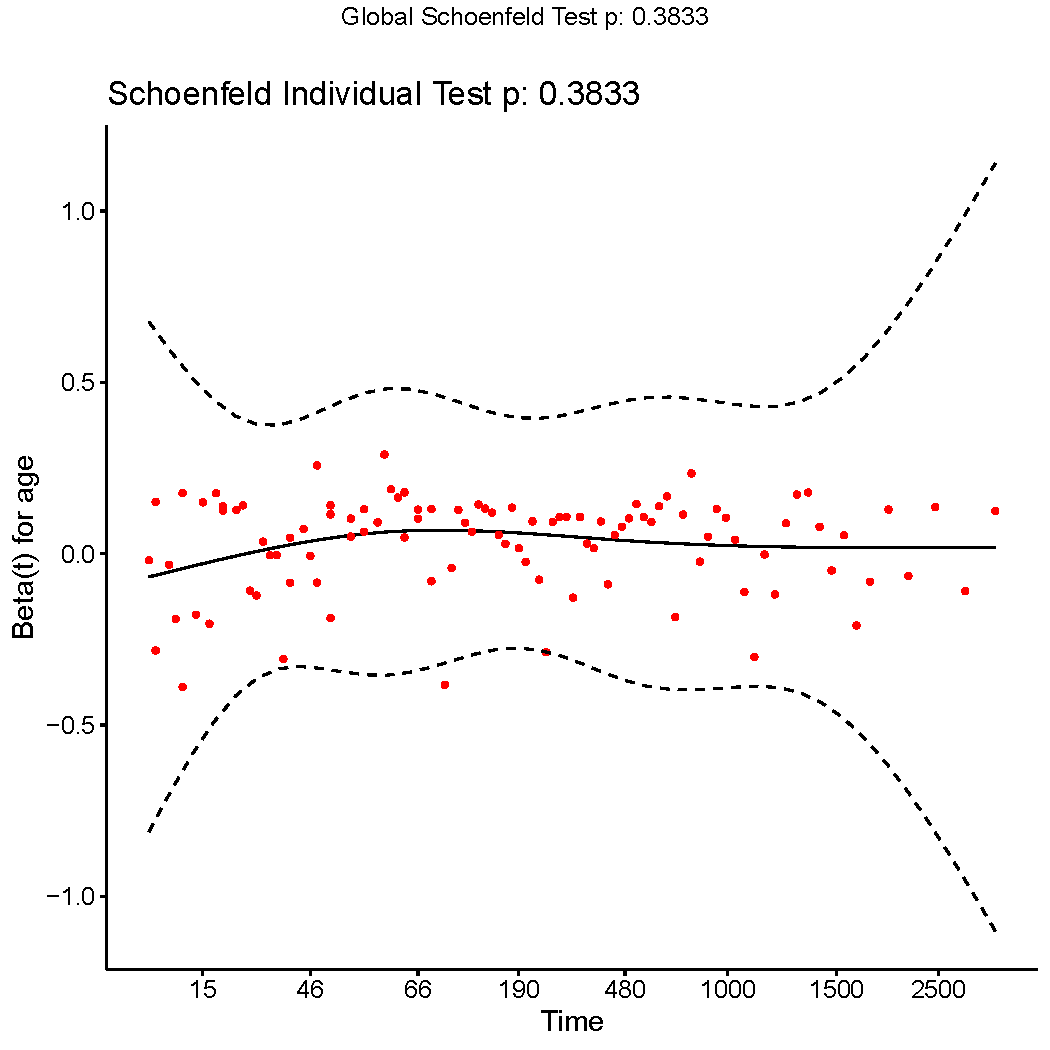
\includegraphics[width=0.7\textwidth]{figures/survival/stanford_cox_age_schoenfeld_residuals}
\vspace{0.2cm}
\caption{
Schoenfeld residual plot for
an univariate Cox model fit to the Stanford heart transplant dataset.
The residuals do not appear dependent on time,
which is supported by the non-significant \pvalue,
and shows that proportional hazards assumption
has been satisfied for this model.
}
\label{fig:cox:schoenfeld_residuals}
\end{figure}

\begin{figure}[H]
\centering
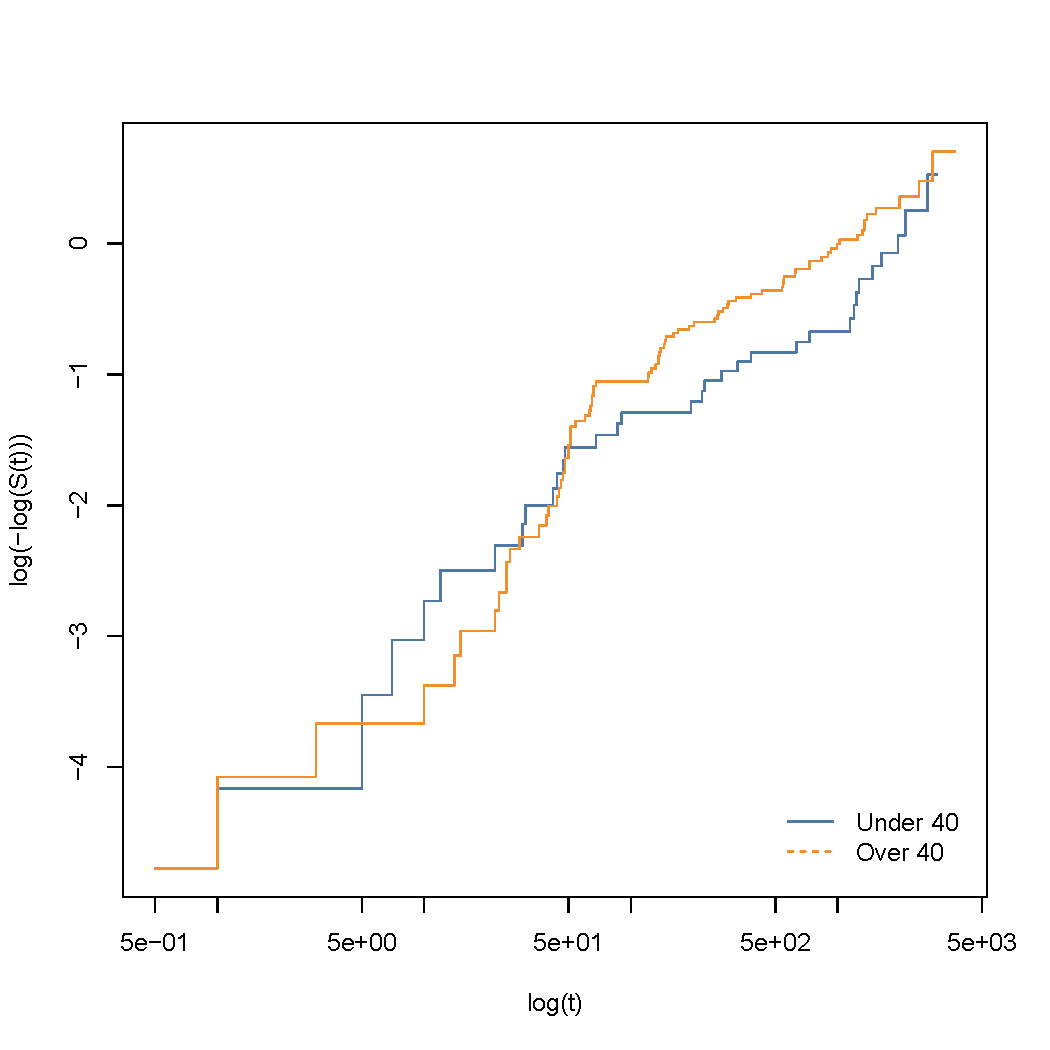
\includegraphics[width=0.7\textwidth]{figures/survival/stanford_cloglog}
\vspace{0.2cm}
\caption{
Complementary log-log plot for categorized patient age
in the Stanford heart transplant dataset.
These curves are not parallel,
the proportional hazards assumption is violated in this variable.
}
\label{fig:stanford_cloglog}
\end{figure}

\begin{figure}[H]
\centering
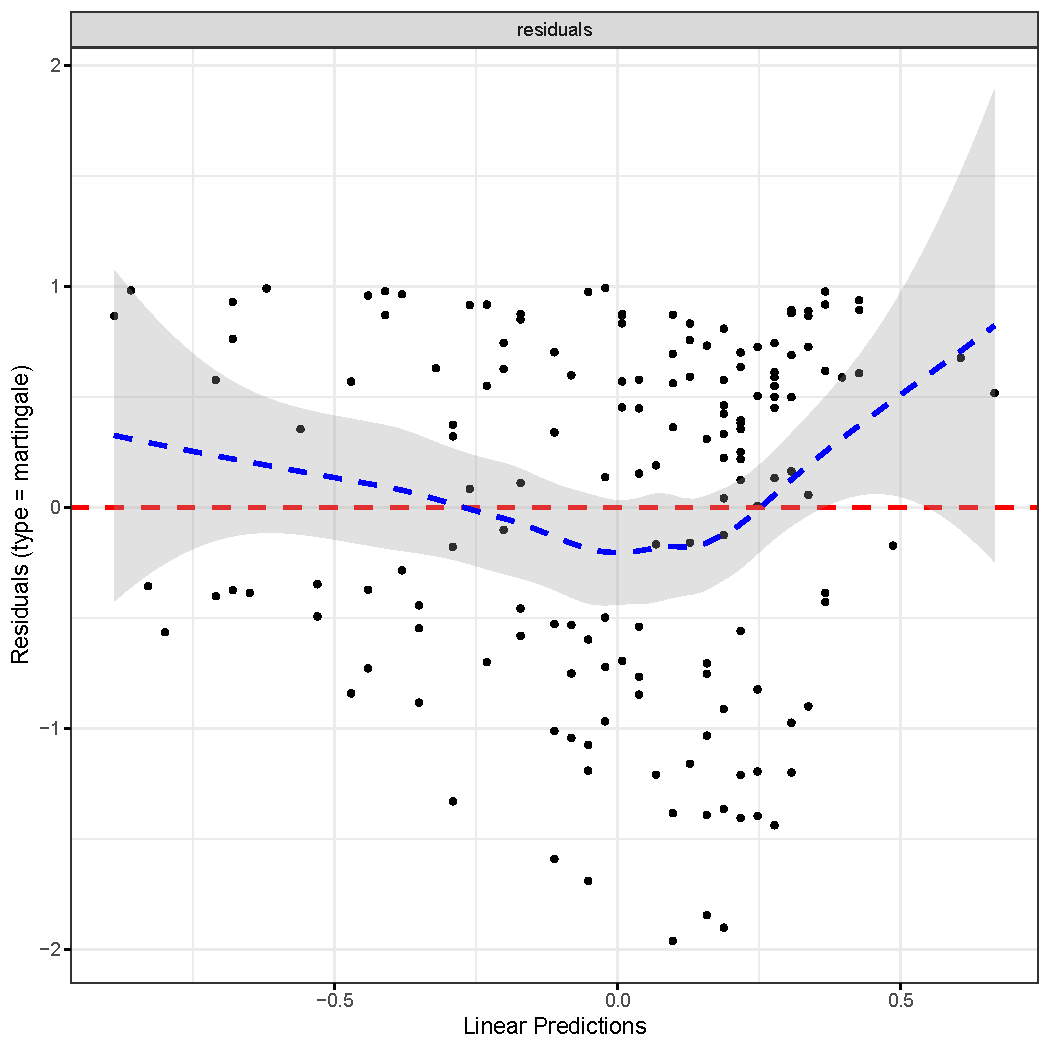
\includegraphics[width=0.7\textwidth]{figures/survival/stanford_cox_age_martingale_residuals}
\vspace{0.2cm}
\caption{
TODO Martingale residuals
}
\label{fig:cox:martingale_residuals}
\end{figure}

\begin{figure}[H]
\centering
  \begin{subfigure}[c]{0.48\textwidth}\centering
  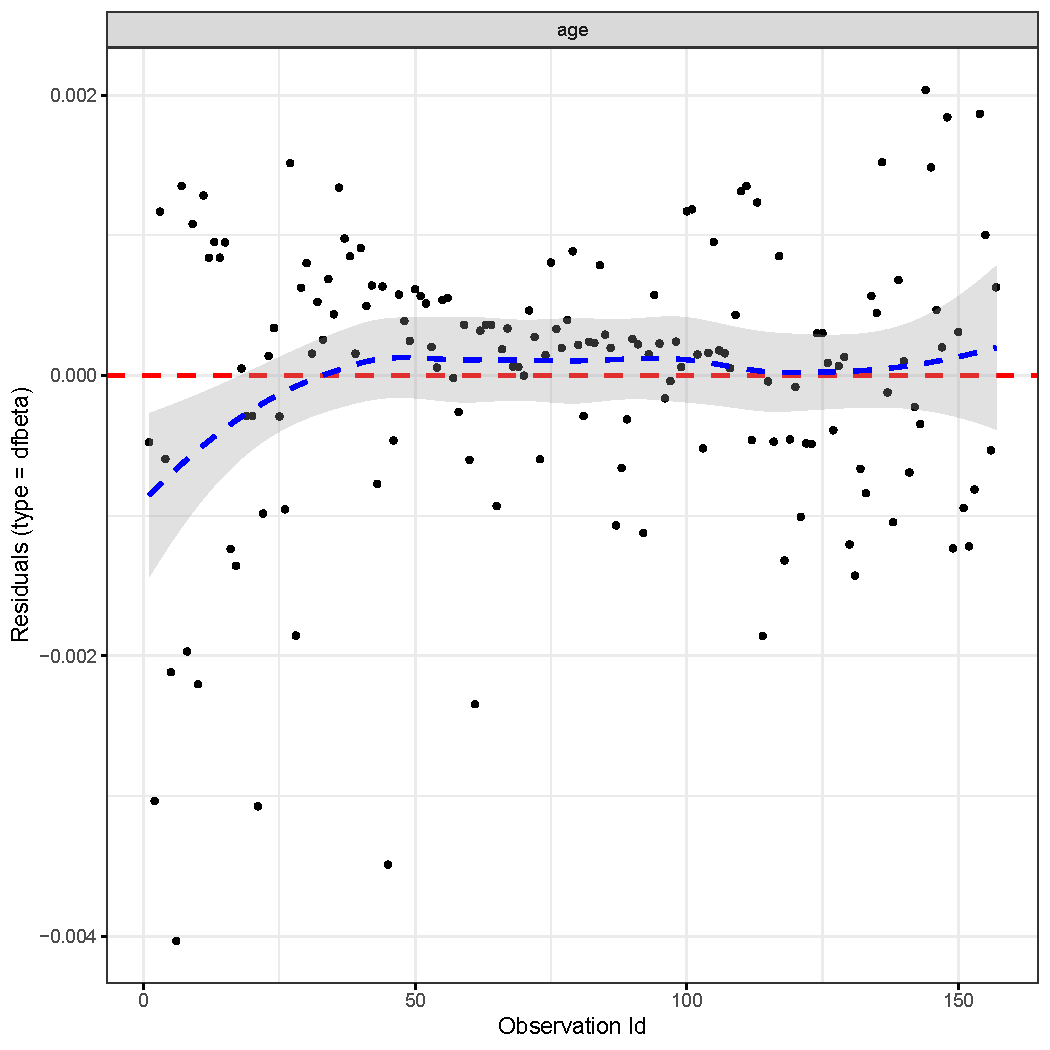
\includegraphics[width=\textwidth]{figures/survival/stanford_cox_age_dfbeta}
  \caption{dfbeta}
  \label{fig:cox:outliers:dfbeta}
  \end{subfigure}
  ~
  \begin{subfigure}[c]{0.48\textwidth}\centering
  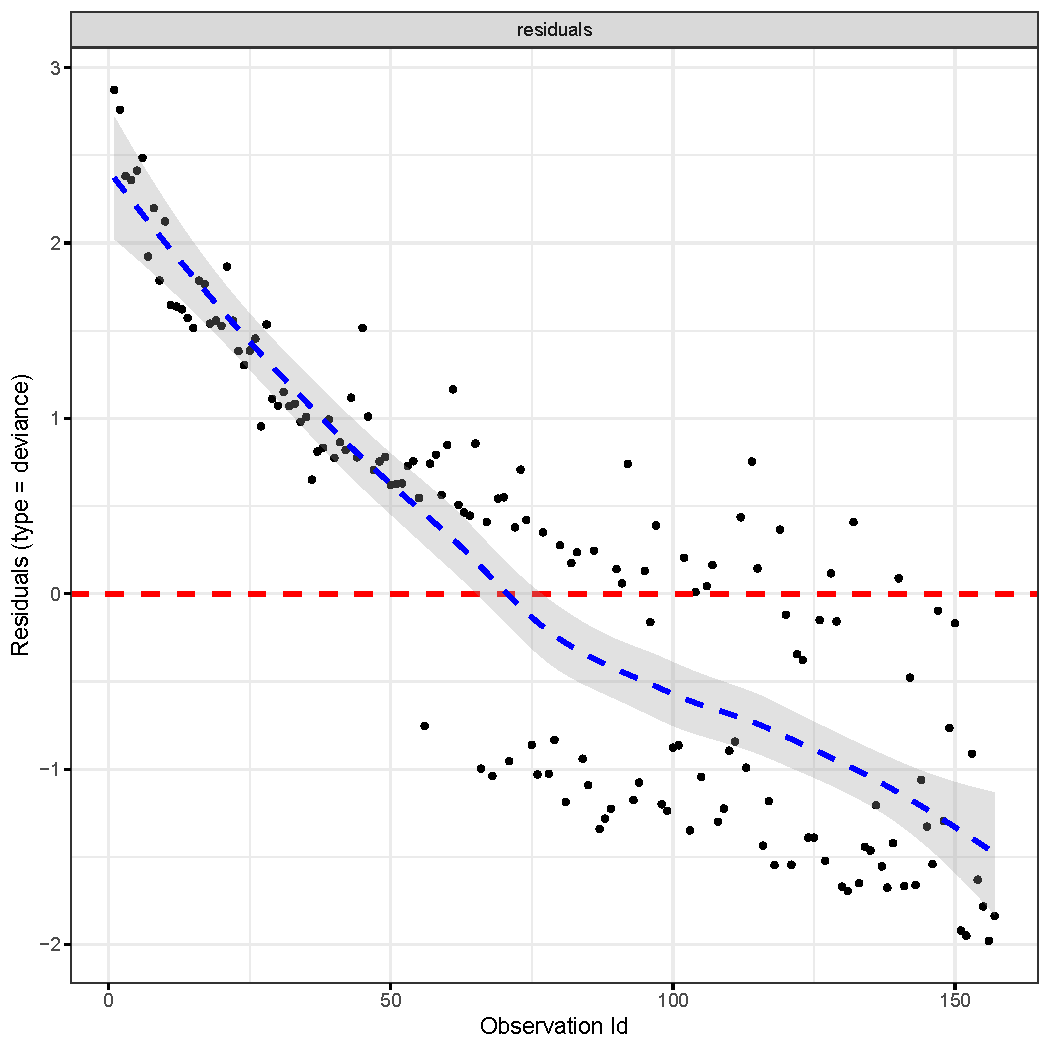
\includegraphics[width=\textwidth]{figures/survival/stanford_cox_age_deviance_residuals}
  \caption{Deviance}
  \label{fig:cox:outliers:deviance}
  \end{subfigure}
\caption{
TODO Outliers
TODO dfbeta and deviance residual plots for
an univariate Cox model fit to the Stanford heart transplant dataset.
}
\label{fig:cox:outliers}
\end{figure}

%%%%%%%%%%%%%%%%%%%%%%%%%%%%%%%%%%%%%%%%%%%%%%%%%%%%%%%%
%%%%%%%%%%%%%%%%%%%%%%%%%%%%%%%%%%%%%%%%%%%%%%%%%%%%%%%%
\section{General Machine Learning Concepts}
\label{additional:ml:general}

%%%%%%%%%%%%%%%%%%%%%%%%%%%%%%%%%%%%%%%%%%%%%%%%%%%%%%%%
\subsection{ROC Curves}
\label{additional:ml:general:eval:ROC}
% TODO
% TODO cite in text \cref{fig:ml:roc}

\begin{figure}[H]
\centering
  \begin{subfigure}[c]{0.48\textwidth}\centering
  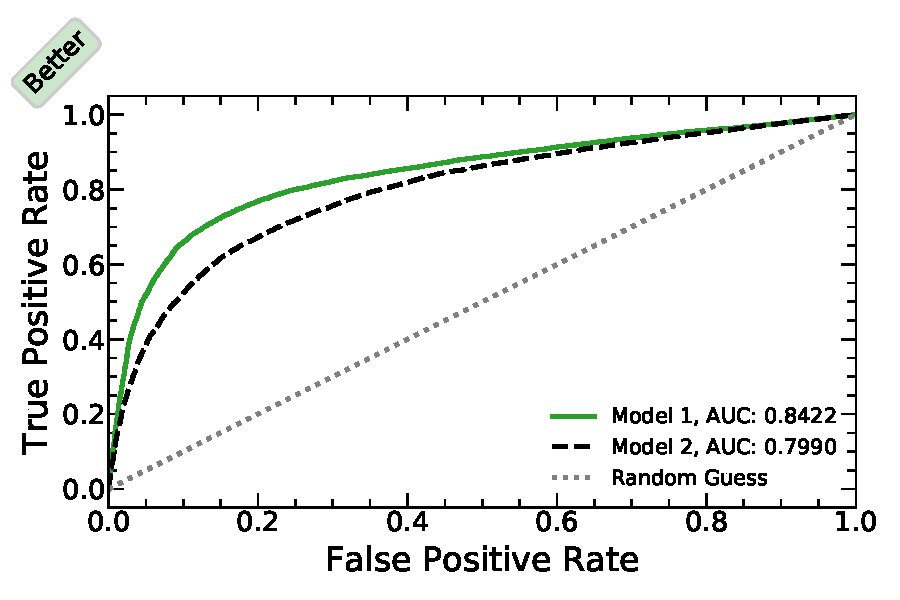
\includegraphics[width=\textwidth,trim={0.18cm 0.3cm 0.18cm 0.3cm},clip]{figures/ml/roc_curves/roc.pdf}% trim={<left> <lower> <right> <upper>}
  \caption{TPR vs FPR}
  \label{fig:ml:roc:standard}
  \end{subfigure}
  ~
  \begin{subfigure}[c]{0.48\textwidth}\centering
  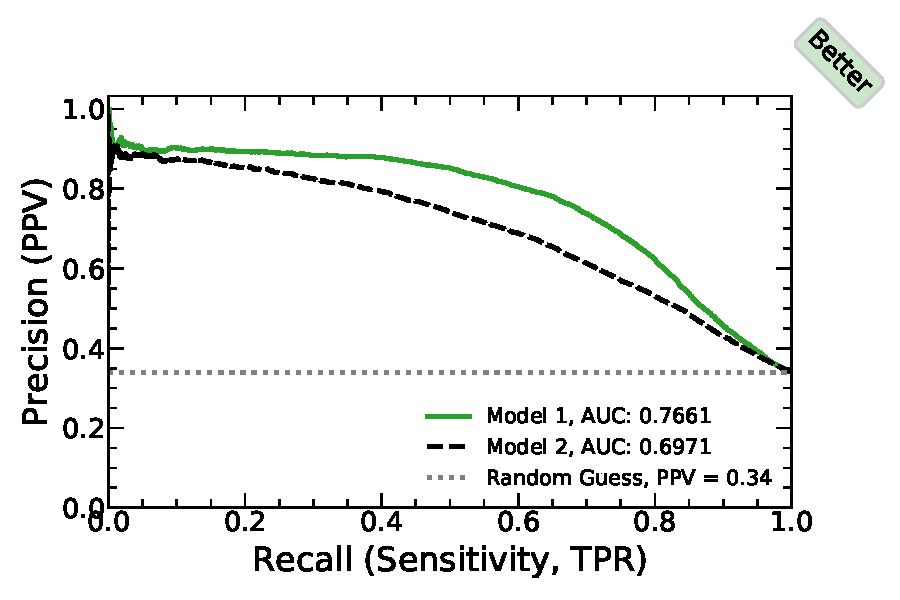
\includegraphics[width=\textwidth,trim={0.18cm 0.3cm 0.18cm 0.3cm},clip]{figures/ml/roc_curves/roc_precision_recall.pdf}% trim={<left> <lower> <right> <upper>}
  \caption{Precision vs Recall}
  \label{fig:ml:roc:precision_recall}
  \end{subfigure}
\caption{
Example ROC curves, generated by \texttt{\href{http://github.com/mepland/roc_curve_demo}{roc\_curve\_demo}}.
Note that model $1$ in solid green outperforms model $2$ when looking at TPR vs FPR and precision vs recall.
The random guess line in the precision vs recall plot is set by the class balance,
in this case the training set contained \SI{34}{\percent} signal.
}
\label{fig:ml:roc}
\end{figure}

%%%%%%%%%%%%%%%%%%%%%%%%%%%%%%%%%%%%%%%%%%%%%%%%%%%%%%%%
\subsection{Selecting a Decision Threshold}
\label{additional:ml:general:eval:decision_threshold}

% include \cref to significance section, if eventually added

In physics we may try to maximize the significance $Z$ of a classifier\footnote{And or
work with the \href{https://en.wikipedia.org/wiki/Neyman\%E2\%80\%93Pearson\_lemma}{Neyman-Pearson framework}.} by
picking an optimal point along the ROC curve to set the decision threshold.
However in data science it is often better to create a payoff matrix of the anticipated
benefits associated with a TP or TN, and costs associated with a FP or FN,
for the particular business case at hand.
The expected value of any decision threshold can quickly be computed
from the payoff matrix elements, $\expvalE{\hat{A} \mid B}$, as

\begin{equation} \label{eq:E_profit}
\expvalE{\text{profit}} = \sum_{A,B} \expvalE{\hat{A} \mid B} P\left(\hat{A} \mid B \right) P\left(B\right),
\end{equation}

\noindent where $A$ and $B$ are any two cases.
The optimal decision threshold can then be found by maximizing $\expvalE{\text{profit}}$.

%%%%%%%%%%%%%%%%%%%%%%%%%%%%%%%%%%%%%%%%%%%%%%%%%%%%%%%%
\subsection{Normalization}
\label{additional:ml:general:normalization}
% TODO normalization of input features (for faster training, more equal regularization), batch renormalization in neural networks

\subsubsection{Batch Renormalization}
\label{additional:ml:general:reg:batch_renorm}
% TODO

%%%%%%%%%%%%%%%%%%%%%%%%%%%%%%%%%%%%%%%%%%%%%%%%%%%%%%%%
\subsection{Loss Functions}
\label{additional:ml:general:loss_func}

% TODO add more loss functions such as log loss, OLS / MSE

\subsubsection{Binary Logistic}
\label{additional:ml:sgeneral:loss_functions:binary_logistic}

In two class, signal $y=1$ and background $y=0$, classification problems the binary logistic function is an appropriate choice of $L$:

\begin{equation} \label{eq:binary_logistic}
L = \sum_{j=1}^{m} \left[y_{j} \ln\left(1 + \exp(-\yhat_{j})\right) +\left(1-y_{j}\right) \ln\left(1 + \exp(\yhat_{j})\right)\right].
\end{equation}

% TODO add more on the information theory aspect

%%%%%%%%%%%%%%%%%%%%%%%%%%%%%%%%%%%%%%%%%%%%%%%%%%%%%%%%
\subsection{Regularization}
\label{additional:ml:general:reg}

\subsubsection{Elastic Net}
\label{additional:ml:general:reg:EN}

L1 and L2 regularization can be used in combination
to take advantage of both of their benefits.
Such a combination is known as the elastic net penalty \cref{eq:elastic_net},
where the combination can be controlled via two $\lambda_{1}$, $\lambda_{2}$ hyperparameters,
or a shared $\lambda$ and mixing parameter $\alpha$.
Compared to LASSO, elastic net does better when given multiple highly correlated features
and is more stable, \ie less dependent on the particular training data.

\begin{equation} \label{eq:elastic_net}
\begin{split}
\Omega_{\text{EN}}\left(\bm{\beta}\right) &= \lambda_{1} \norm{\bm{\beta}} + \lambda_{2} \norm{\bm{\beta}}^{2}\\
&= \lambda \left( \alpha\norm{\bm{\beta}} + \left(1-\alpha\right)\norm{\bm{\beta}}^{2} \right)
\end{split}
\end{equation}

% TODo connections to SVM (https://en.wikipedia.org/wiki/Elastic_net_regularization#Reduction_to_support_vector_machine)

\subsubsection{Drop Out}
\label{additional:ml:general:reg:Drop}
% TODO

\subsubsection{Early Stopping}
\label{additional:ml:general:reg:early_stopping}
% TODO
% TODO ref in text \cref{fig:additional:ml:general:early_stopping}

\begin{figure}[H]
\centering
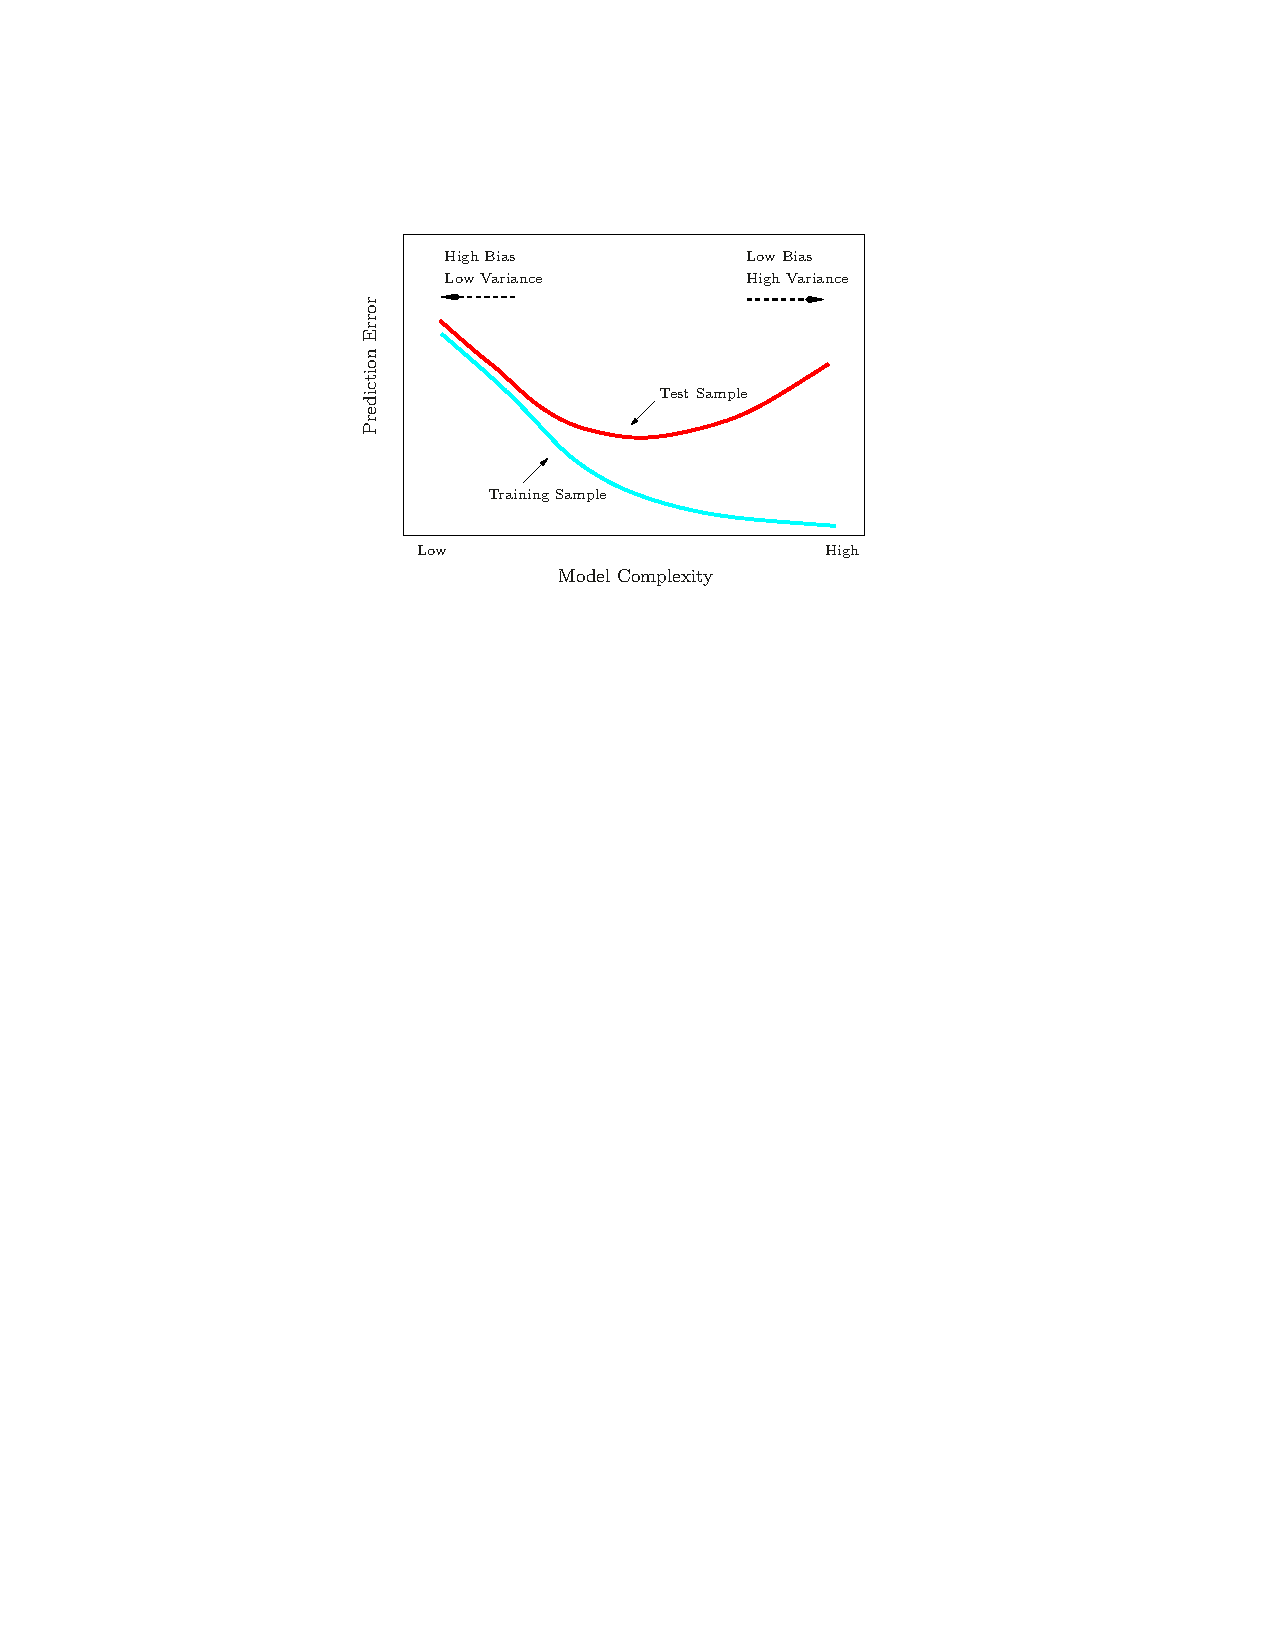
\includegraphics[width=0.8\textwidth]{figures/ml/test_train_err_curves.pdf}
\caption{
Illustrated effects of increasing model complexity on the error rates for the test and train sets \cite{HastieTF09}.
Early stopping would halt the training process when the test (or better yet, validation) set error stops decreasing.
This is also another example of the bias-variance tradeoff in action.
}
\label{fig:additional:ml:general:early_stopping}
\end{figure}

%%%%%%%%%%%%%%%%%%%%%%%%%%%%%%%%%%%%%%%%%%%%%%%%%%%%%%%%
\subsection{Silhouette Value}
\label{additional:ml:general:silhouette}
% TODO

%%%%%%%%%%%%%%%%%%%%%%%%%%%%%%%%%%%%%%%%%%%%%%%%%%%%%%%%
\subsection{Exploration-Exploitation Tradeoff}
\label{additional:ml:general:EE_tradeoff}
% TODO
 
\subsubsection{Bayesian Bandits}
\label{additional:ml:general:EE_tradeoff:BB}
% TODO

%%%%%%%%%%%%%%%%%%%%%%%%%%%%%%%%%%%%%%%%%%%%%%%%%%%%%%%%
%%%%%%%%%%%%%%%%%%%%%%%%%%%%%%%%%%%%%%%%%%%%%%%%%%%%%%%%
\section{Unsupervised Learning}
\label{additional:unsupervised}

%%%%%%%%%%%%%%%%%%%%%%%%%%%%%%%%%%%%%%%%%%%%%%%%%%%%%%%%
\subsection{Bayesian Optimization}
\label{additional:unsupervised:BO}

Frequently we are fortunate enough to have a fairly explicit form of
the objective function $S\left(\bm{\beta}\right)$ to be optimized in order to solve a problem.
However, when $S\left(\bm{\beta}\right)$ is not well known, is expensive to compute, or is not differentiable,
the usual gradient based approaches, such as SGD and Newton's method, break down.
In these cases ``black box''\footnote{Black box as in
we do not have a closed-form expression for $S$, or know $\grad S$.}\footnote{Evolutionary algorithms
and some tree based methods \cite{Hutter2011,Hutter2014}
are other examples of black box optimizers.} methods,
such as Bayesian optimization, may be used instead.

In Bayesian optimization \cite{Brochu2010,1301.1942,Borisyak},
we begin by assuming some reasonable prior distribution for $S$,
typically in the form of a smooth Gaussian process (GP) fit
to an initial random sample of $\bm{\beta}$, $S\left(\bm{\beta}\right)$ points.
GPs \cref{eq:additional:unsupervised:BO:GP} are
extensions of Gaussian distributions which return a Gaussian at any point along their domain.
They are parameterized by a mean function\footnote{For convenience,
the prior $m\left(\bm{x}\right)$ is usually assumed to be zero, $m\left(\bm{x}\right)=0$.}, $m\left(\bm{x}\right)$,
and covariance function, $k\left(\bm{x}_{i}, \bm{x}_{j}\right)$,
\ie kernel\footnote{The kernel of the GP is a hyperparameter to be chosen in advance.
Standard kernel choices include
the radial basis function kernel $k\left(\bm{x}_{i}, \bm{x}_{j}\right) = \exp\left(-\frac{1}{2\sigma^{2}}\norm{\bm{x}_{i}-\bm{x}{j}}^{2}\right)$,
Mat\'{e}rn kernel,
and white noise kernel $k\left(\bm{x}_{i}, \bm{x}_{j}\right) \propto \delta_{ij}$.},
instead of a constant mean $\mu$ and variance $\sigma^{2}$.
An illustration of a GP is provided in \cref{fig:additional:unsupervised:BO:GP_ex}.

\begin{equation}\label{eq:additional:unsupervised:BO:GP}
f\left(\bm{x}\right) \sim \mathcal{GP}\left(m\left(\bm{x}\right), k\left(\bm{x}_{i}, \bm{x}_{j}\right)\right).
\end{equation}

\begin{figure}
\centering
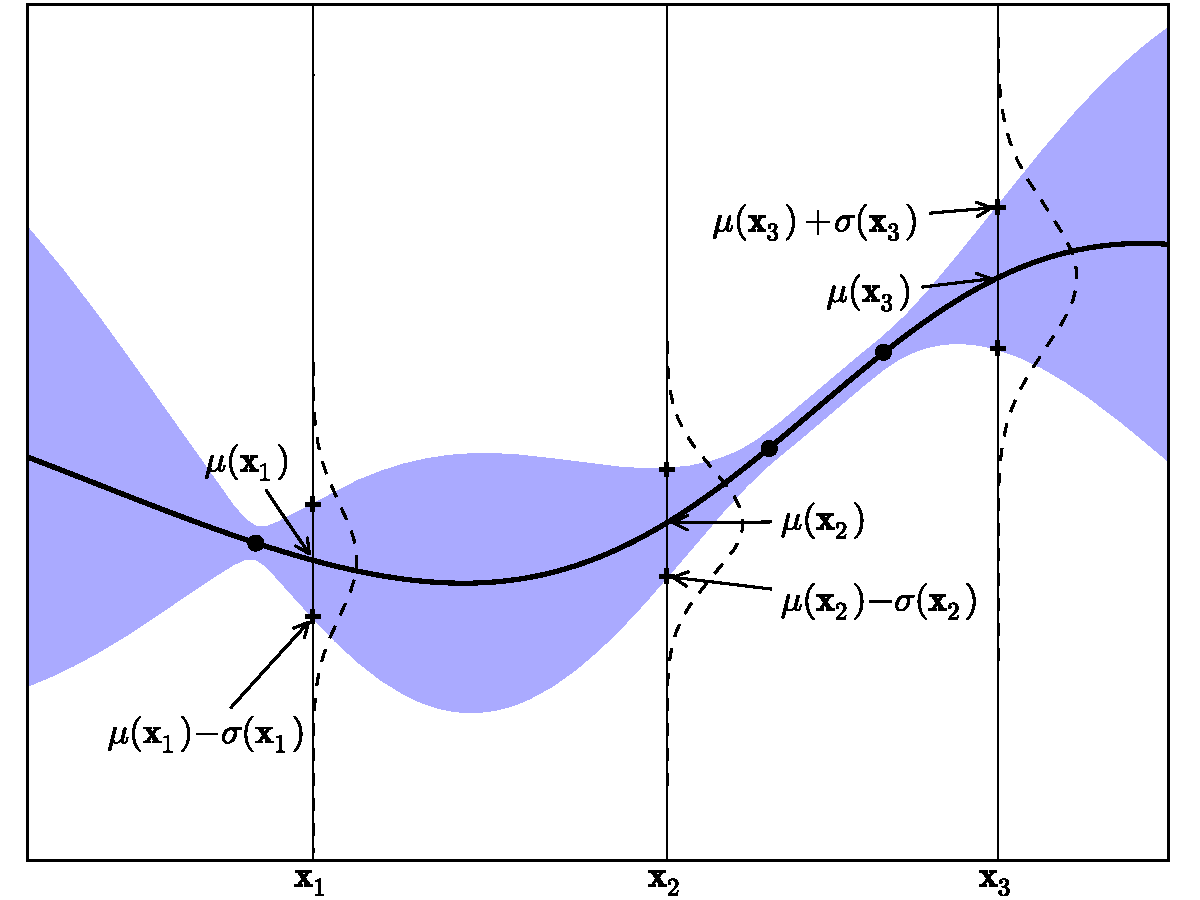
\includegraphics[width=0.85\textwidth]{figures/ml/gp.pdf}
\caption{
Illustration of a Gaussian process (GP) in 1D \cite{Brochu2010}.
Note that at any point $\bm{x}_{1}$, $\bm{x}_{2}$, $\bm{x}_{3}$ the GP
returns a Gaussian distribution characterizing the estimated mean and uncertainty on the
unknown true function, \ie the objective function $S\left(\bm{\beta}\right)$ in the case of Bayesian optimization.
}
\label{fig:additional:unsupervised:BO:GP_ex}
\end{figure}

From the estimated GP prior distribution, Bayesian optimization
operates by iteratively sampling $S\left(\bm{\beta}\right)$ and updating the posterior distribution
as each new point of information is gained.
An acquisition function TODO

% TODO how exactly is the GP updated?
% TODO for acquisition function read Brochu2010 section 2.3
% TODO mention exploration-exploitation tradeoff, discuss details in own section

% TODO Bayesian optimization functionality provided by \skopt \cite{scikit-optimize}

% TODO ref fig in text: \cref{fig:additional:unsupervised:BO:BO_ex}
\begin{figure}
\centering
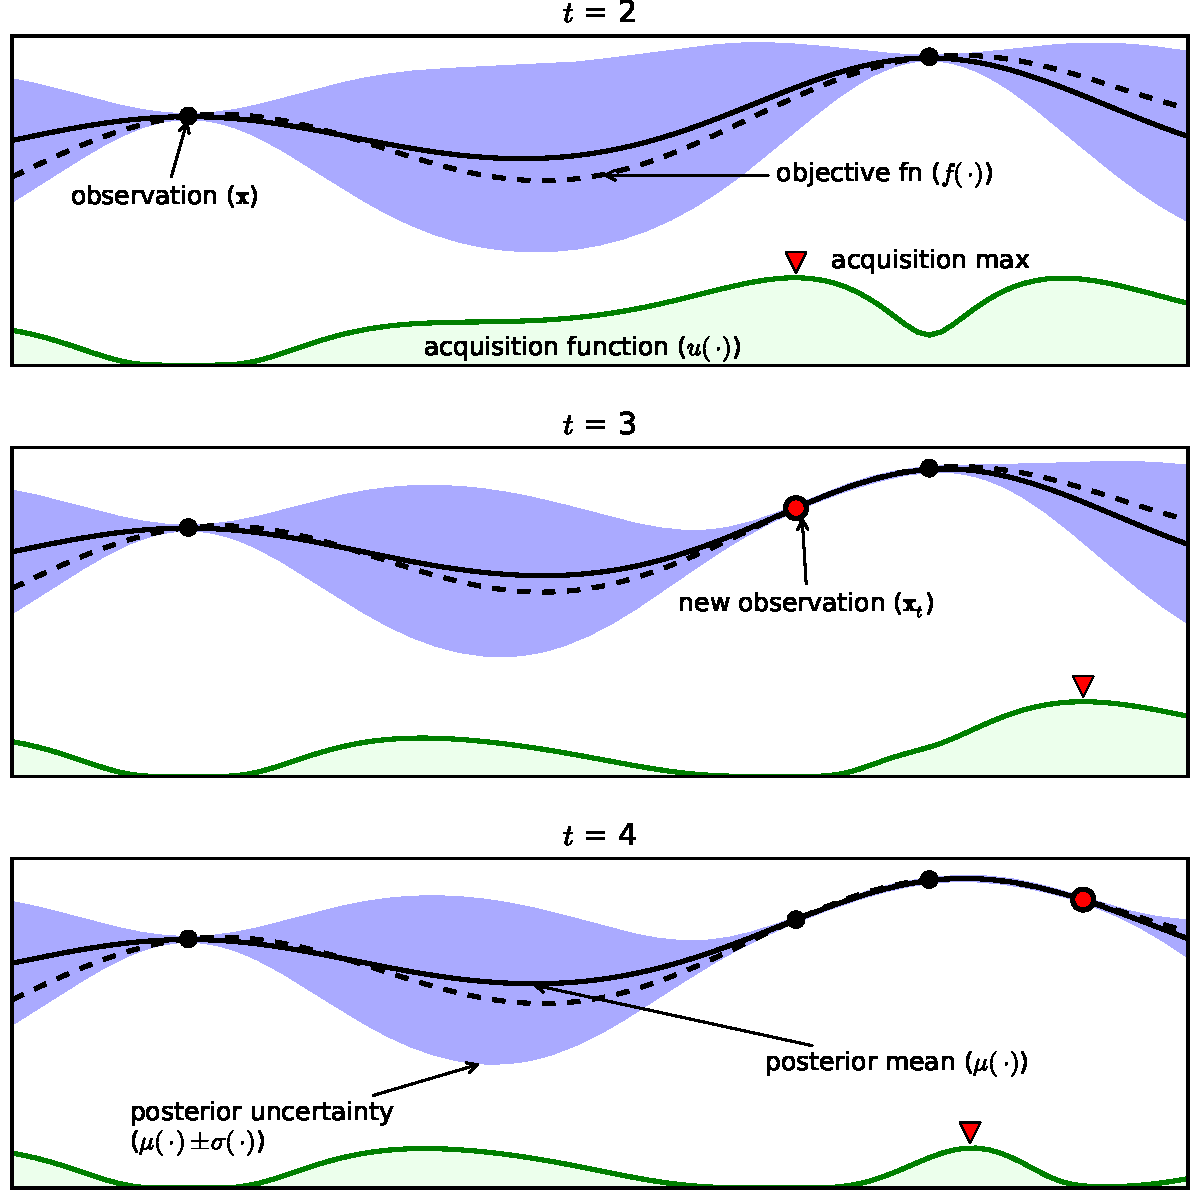
\includegraphics[width=0.85\textwidth]{figures/ml/toyGPtext3.pdf}
\caption{
Illustration of Bayesian optimization in a toy 1D problem \cite{Brochu2010}.
TODO
}
\label{fig:additional:unsupervised:BO:BO_ex}
\end{figure}

% TODO remember to read Brochu2010 section 5

%%%%%%%%%%%%%%%%%%%%%%%%%%%%%%%%%%%%%%%%%%%%%%%%%%%%%%%%
\subsection{Gaussian Mixture Model (GMM)}
\label{additional:unsupervised:GMM}
% TODO

%%%%%%%%%%%%%%%%%%%%%%%%%%%%%%%%%%%%%%%%%%%%%%%%%%%%%%%%
\subsection{\texorpdfstring{$\epsilon$}{epsilon}-Means}
\label{additional:unsupervised:epsilonMean}
% TODO

%%%%%%%%%%%%%%%%%%%%%%%%%%%%%%%%%%%%%%%%%%%%%%%%%%%%%%%%
\subsection{Louvain Method}
\label{additional:unsupervised:louvain}
% TODO

%%%%%%%%%%%%%%%%%%%%%%%%%%%%%%%%%%%%%%%%%%%%%%%%%%%%%%%%
\subsection{Variational Autoencoders (VAE)}
\label{additional:unsupervised:VAE}
% TODO

%%%%%%%%%%%%%%%%%%%%%%%%%%%%%%%%%%%%%%%%%%%%%%%%%%%%%%%%
\subsection{Support Vector Clustering}
\label{additional:unsupervised:SVC}
% TODO


%%%%%%%%%%%%%%%%%%%%%%%%%%%%%%%%%%%%%%%%%%%%%%%%%%%%%%%%
%%%%%%%%%%%%%%%%%%%%%%%%%%%%%%%%%%%%%%%%%%%%%%%%%%%%%%%%
\section{Supervised Learning}
\label{additional:supervised}

%%%%%%%%%%%%%%%%%%%%%%%%%%%%%%%%%%%%%%%%%%%%%%%%%%%%%%%%
\subsection{Recursive Neural Networks (RNN)}
\label{additional:supervised:RNN}
% TODO

\subsubsection{Long Short Term Memory (LSTM)}
\label{additional:supervised:RNN:LSTM}
% TODO

%%%%%%%%%%%%%%%%%%%%%%%%%%%%%%%%%%%%%%%%%%%%%%%%%%%%%%%%
\subsection{Convolutional Neural Networks (CNN)}
\label{additional:supervised:CNN}
% TODO

%%%%%%%%%%%%%%%%%%%%%%%%%%%%%%%%%%%%%%%%%%%%%%%%%%%%%%%%
\subsection{Adversarial Networks}
\label{additional:supervised:AN}
% TODO
% TODO abbreviate as AN?

%%%%%%%%%%%%%%%%%%%%%%%%%%%%%%%%%%%%%%%%%%%%%%%%%%%%%%%%
\subsection{Variational Autoencoders (VAE)}
\label{additional:supervised:VAE}
% TODO

\subsection{Learning Vector Quantization (LVQ)}
\label{additional:supervised:kNN:LVQ}
% TODO


%%%%%%%%%%%%%%%%%%%%%%%%%%%%%%%%%%%%%%%%%%%%%%%%%%%%%%%%
%%%%%%%%%%%%%%%%%%%%%%%%%%%%%%%%%%%%%%%%%%%%%%%%%%%%%%%%
\section{Miscellaneous}
\label{additional:misc}

%%%%%%%%%%%%%%%%%%%%%%%%%%%%%%%%%%%%%%%%%%%%%%%%%%%%%%%%
\subsection{Checking \texorpdfstring{$m$}{m} for the Model}
\label{additional:misc:enough_data}
% TODO
% TODO ref in text \cref{fig:additional:misc:enough_data}

\begin{figure}
\centering
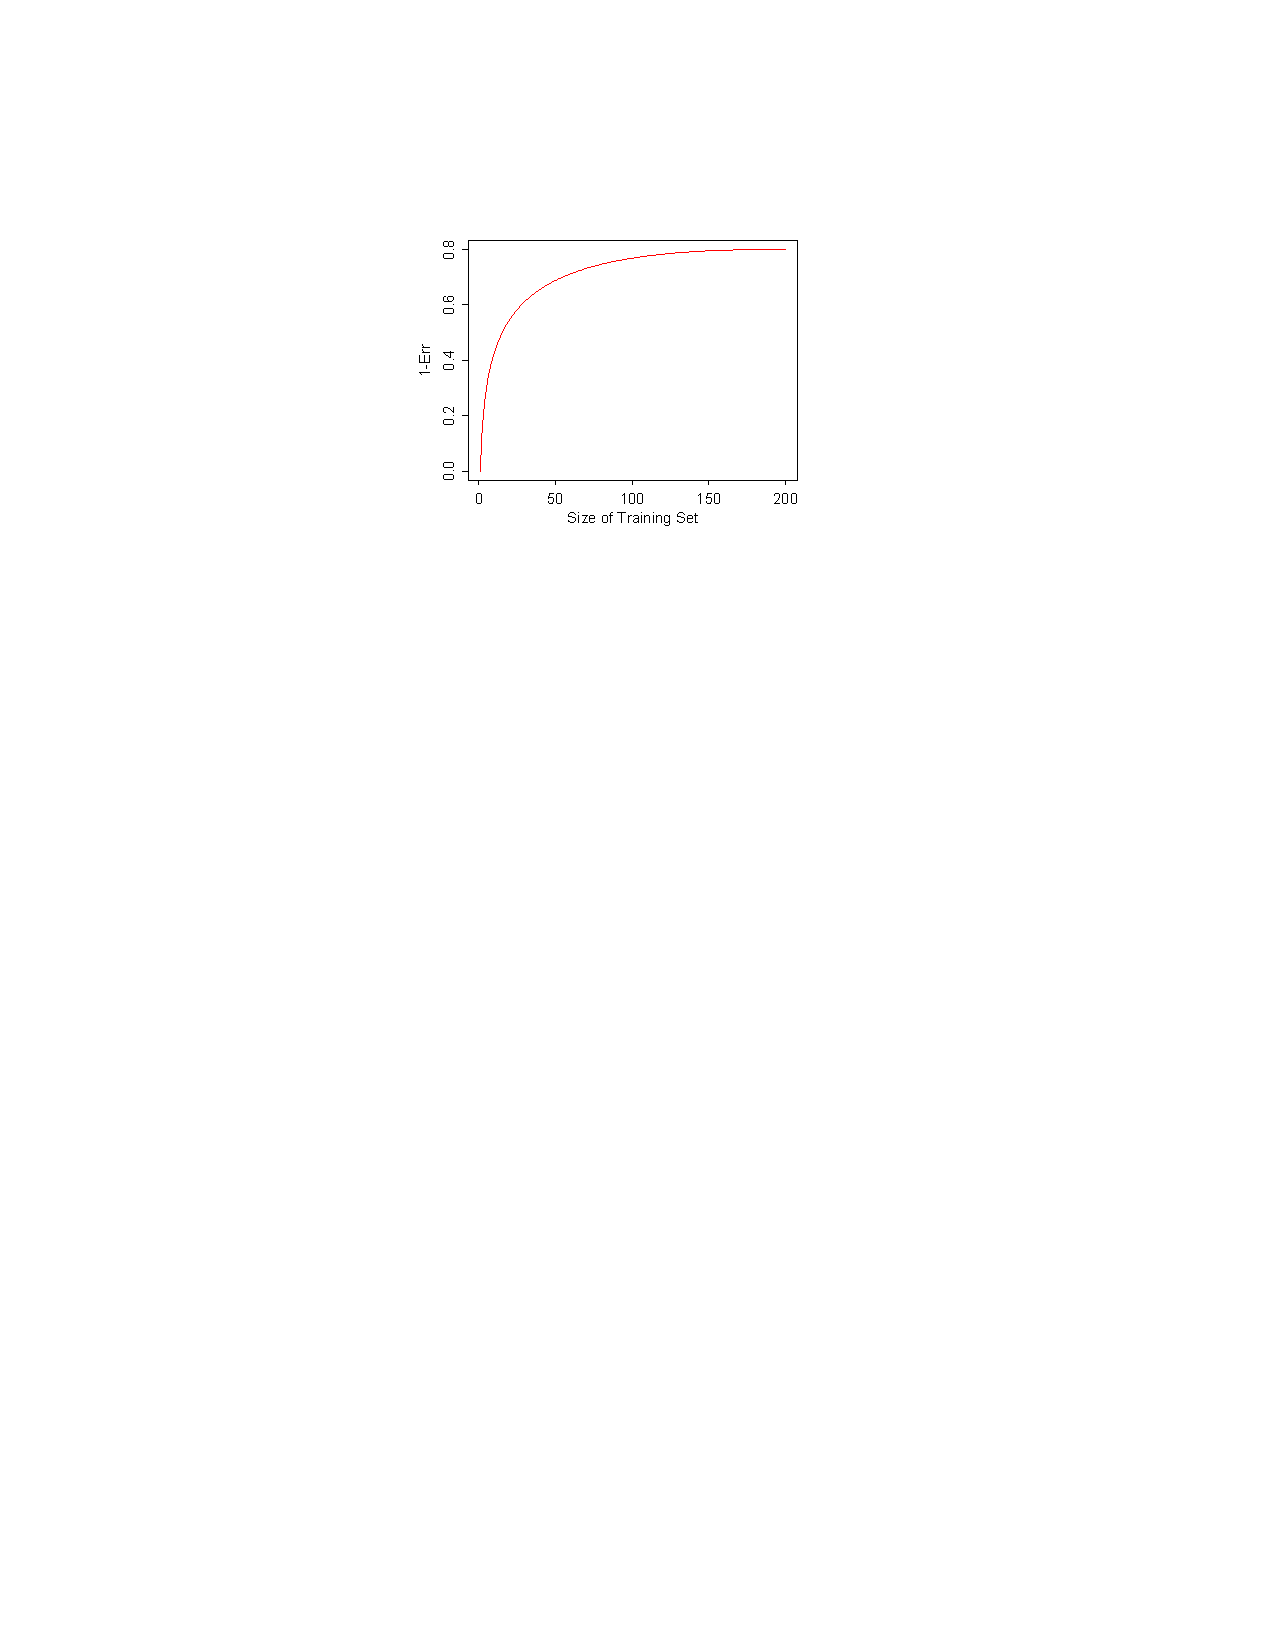
\includegraphics[width=0.8\textwidth]{figures/ml/acc_vs_m.pdf}
\caption{
Illustration of the decrease in classification error rate
with larger sets of training data \cite{HastieTF09}.
By artificially limiting the available number of data points $m$,
one can create a similar curve to verify that
there is enough statistics in the training data
for the complexity of the model under consideration.
Ideally the curve should reach a clear asymptote before the maximum $m$ is used.
}
\label{fig:additional:misc:enough_data}
\end{figure}

%%%%%%%%%%%%%%%%%%%%%%%%%%%%%%%%%%%%%%%%%%%%%%%%%%%%%%%%
\subsection{Factor Analysis}
\label{additional:misc:factor_ana}
% TODO

%%%%%%%%%%%%%%%%%%%%%%%%%%%%%%%%%%%%%%%%%%%%%%%%%%%%%%%%
\subsection{Optimization and Lagrange Multipliers}
\label{additional:misc:opt}
% TODO

%%%%%%%%%%%%%%%%%%%%%%%%%%%%%%%%%%%%%%%%%%%%%%%%%%%%%%%%
\subsection{Information Theory}
\label{additional:misc:info_theory}
% TODO
% TODO Entropy, significance of bits

%%%%%%%%%%%%%%%%%%%%%%%%%%%%%%%%%%%%%%%%%%%%%%%%%%%%%%%%
\subsection{Modulo Operations}
\label{additional:misc:modulo}

\begin{subequations}\label{eq:additional:misc:modulo}
\begin{align}
\left(A~\text{mod}~C\right)~\text{mod}~C &= A~\text{mod}~C, \label{eq:misc:additional:modulo:basic} \\
\left(A \pm B\right)~\text{mod}~C &= \left(A~\text{mod}~C \pm B~\text{mod}~C\right)~\text{mod}~C, \label{eq:misc:additional:modulo:pm} \\
\left(A \times B\right)~\text{mod}~C &= \left(A~\text{mod}~C \times B~\text{mod}~C\right)~\text{mod}~C, \label{eq:misc:additional:modulo:multiplication} \\
A^{B}~\text{mod}~C &= \left(\left(A~\text{mod}~C\right)^{B}\right)~\text{mod}~C. \label{eq:misc:additional:modulo:exp}
\end{align}
\end{subequations}

}
%%%%%%%%%%%%%%%%%%%%%%%%%%%%%%%%%%%%%%%%%%%%%%%%%%%%%%%%
%%%%%%%%%%%%%%%%%%%%%%%%%%%%%%%%%%%%%%%%%%%%%%%%%%%%%%%%
%%%%%%%%%%%%%%%%%%%%%%%%%%%%%%%%%%%%%%%%%%%%%%%%%%%%%%%%
\chapter{Probability Distributions}
\label{dist}

% Place these distributions first as they are simple and keep the interesting ones together on the next page
\begin{figure}
  \centering
  \savebox{\largestimage}{
    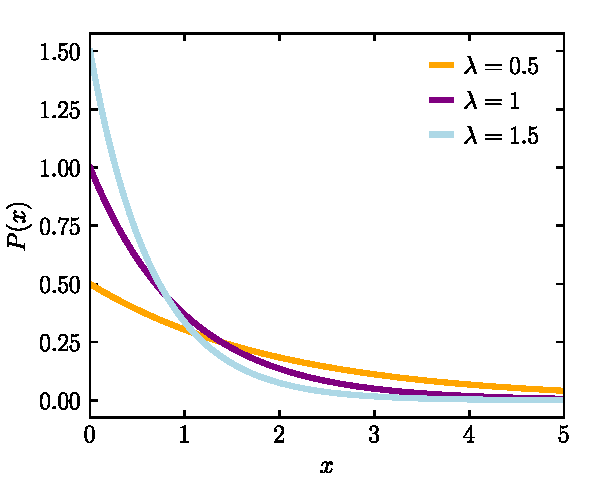
\includegraphics[width=0.47\textwidth]{figures/stats/dist/exp_pdf}
  }% Store largest image in a box

  \begin{subfigure}[b]{0.48\textwidth}\centering
    \raisebox{\dimexpr.5\ht\largestimage-.5\height}{% Adjust vertical height of smaller image
      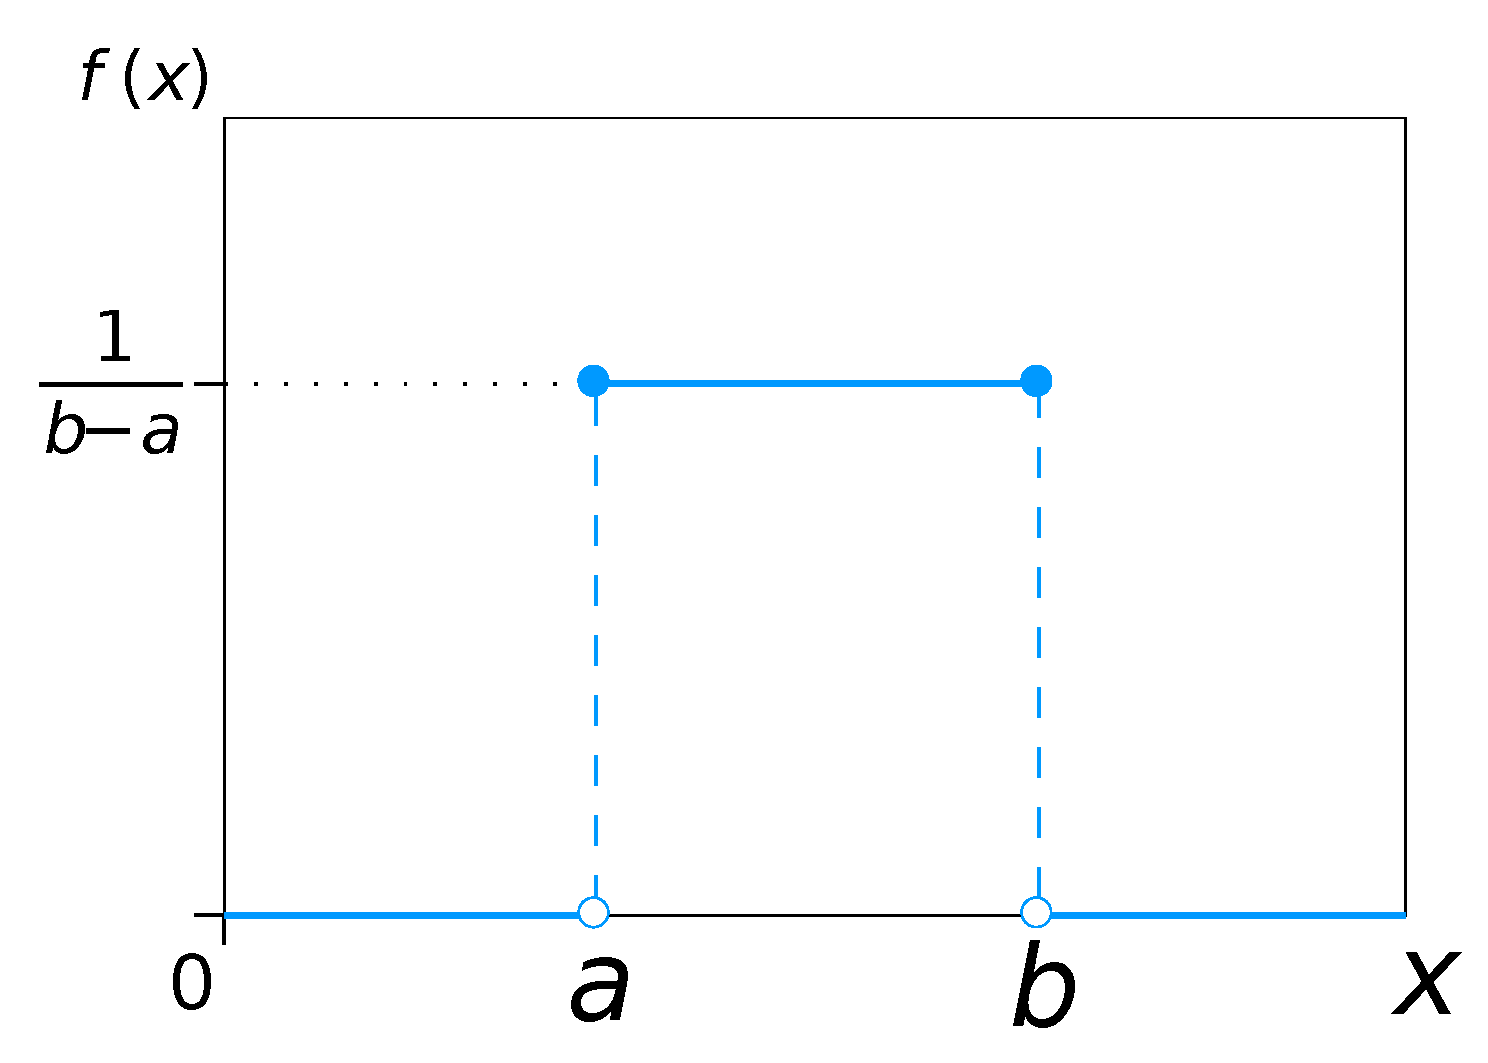
\includegraphics[width=\textwidth]{figures/stats/dist/uniform_pdf}}
  \caption{Uniform Distribution PDF}
  \label{fig:dist:uniform}
  \end{subfigure}
  ~
  \begin{subfigure}[b]{\wd\largestimage}\centering
    \usebox{\largestimage}
  \caption{Exponential Distribution PDF}
  \label{fig:dist:exp}
  \end{subfigure}
\caption{
Uniform and exponential distribution PDFs,
by \href{https://en.wikipedia.org/wiki/File:Uniform_Distribution_PDF_SVG.svg}{AnonMoos}
and \href{https://en.wikipedia.org/wiki/File:Exponential_probability_density.svg}{AkanoToE}.
\label{fig:dist:uniform_exp}
}
\end{figure}

\begin{figure}
  \centering
  \savebox{\largestimage}{
    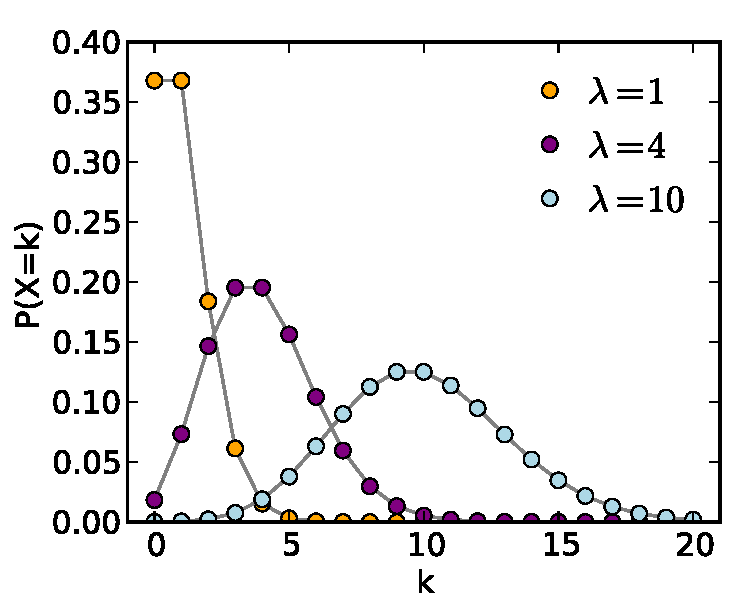
\includegraphics[width=0.47\textwidth]{figures/stats/dist/poisson_pmf}
  }% Store largest image in a box

  \begin{subfigure}[b]{\wd\largestimage}\centering
    \raisebox{\dimexpr.5\ht\largestimage-.5\height}{% Adjust vertical height of smaller image
      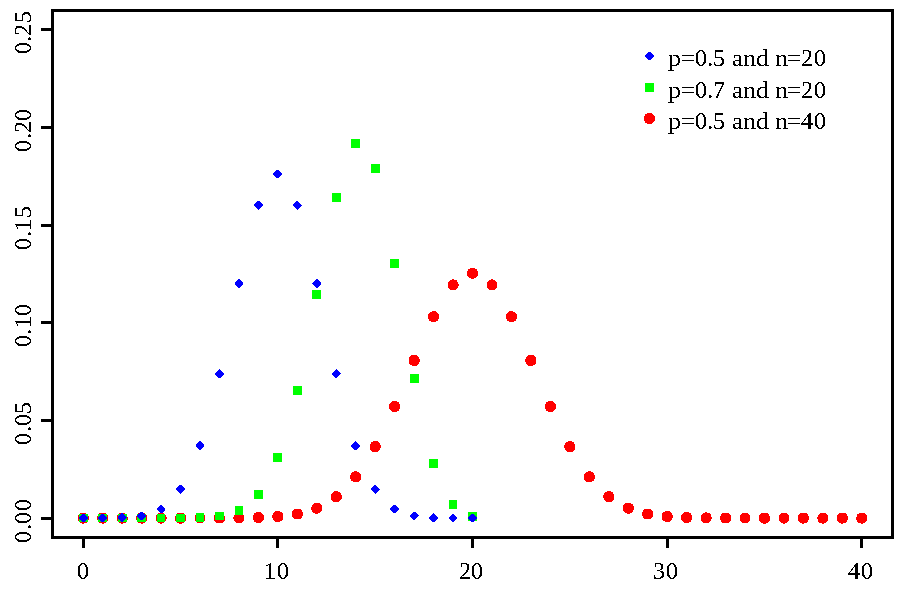
\includegraphics[width=\textwidth]{figures/stats/dist/binomial_pmf}}
  \caption{Binomial Distribution PMF}
  \label{fig:dist:binomial}
  \end{subfigure}
  ~
  \begin{subfigure}[b]{0.48\textwidth}\centering
    \usebox{\largestimage}
  \caption{Poisson Distribution PMF}
  \label{fig:dist:poisson}
  \end{subfigure}
\caption{
Binomial and Poisson distribution PMFs,
by \href{https://en.wikipedia.org/wiki/File:Binomial_distribution_pmf.svg}{Tayste}
and \href{https://en.wikipedia.org/wiki/File:Poisson_pmf.svg}{Skbkekas}.
Both plots have $k$ on the $x$-axis and $P$ on the $y$-axis, and curves for various $n$ and $p$, or $\lambda$.
\label{fig:dist:binomial_poisson}
}
\end{figure}

\begin{figure}
  \centering
  \savebox{\largestimage}{
    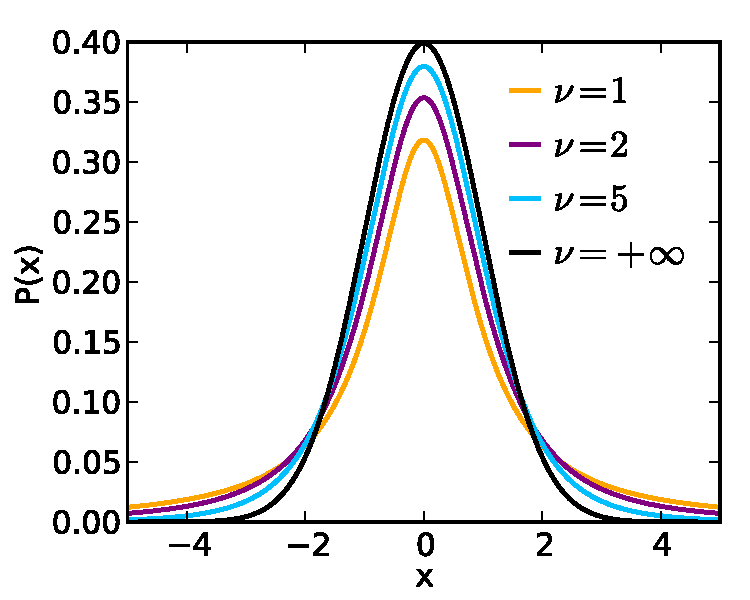
\includegraphics[width=0.47\textwidth]{figures/stats/dist/student_t_pdf}
  }% Store largest image in a box

  \begin{subfigure}[b]{0.48\textwidth}\centering
    \raisebox{\dimexpr.5\ht\largestimage-.5\height}{% Adjust vertical height of smaller image
      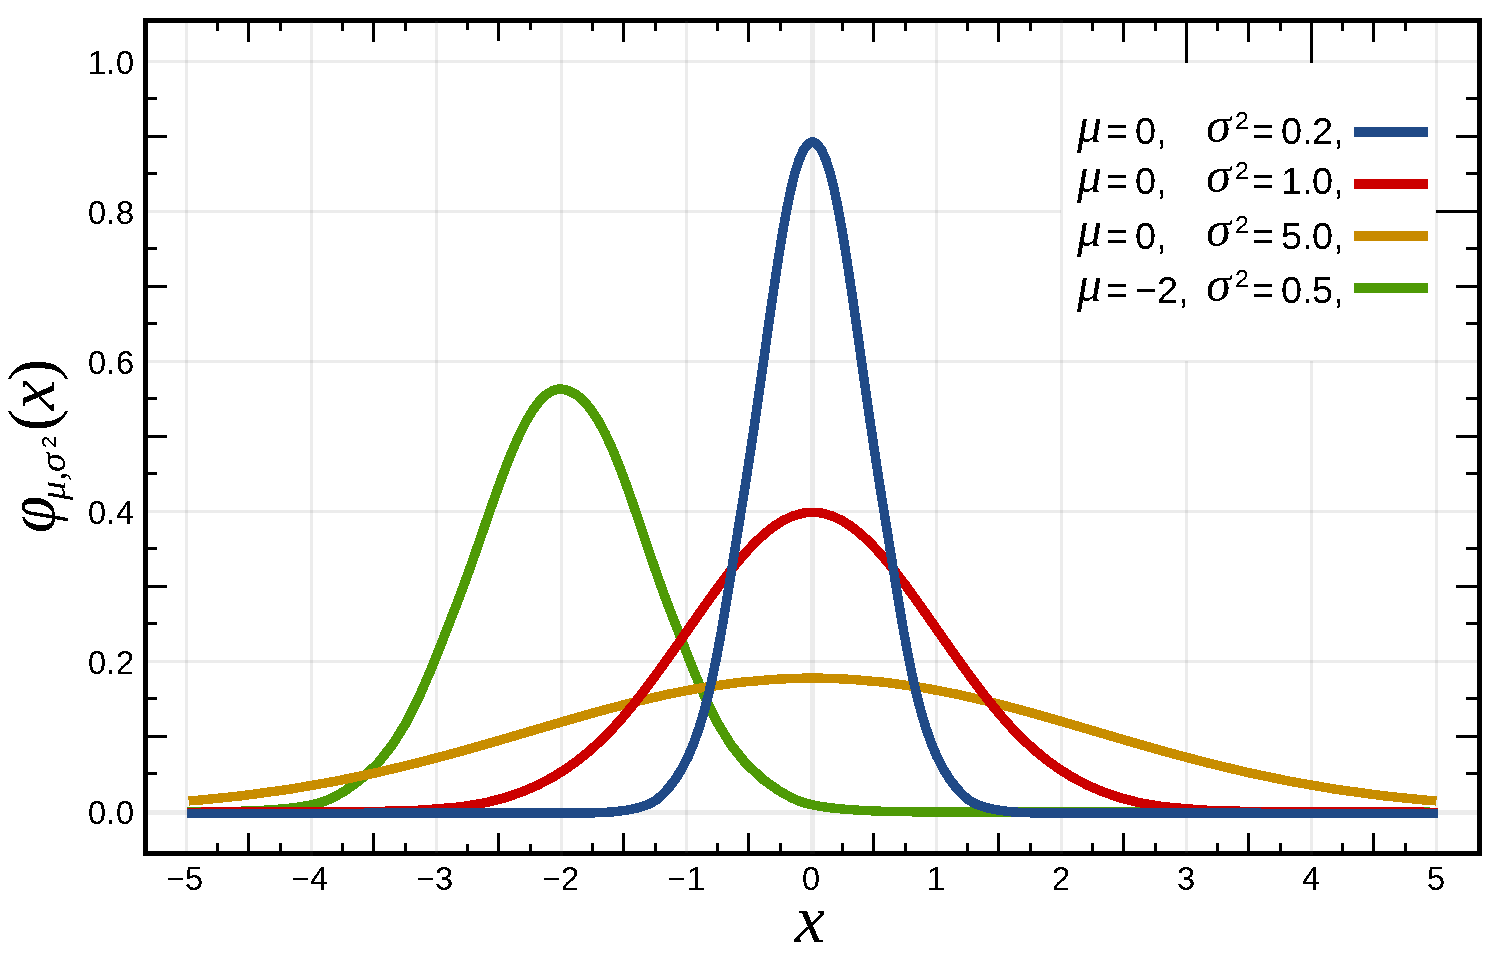
\includegraphics[width=\textwidth]{figures/stats/dist/gaussian_pdf}}
  \caption{Gaussian Distribution PDF}
  \label{fig:dist:gaus}
  \end{subfigure}
  ~
  \begin{subfigure}[b]{\wd\largestimage}\centering
    \usebox{\largestimage}
  \caption{Student's $t$-Distribution PDF}
  \label{fig:dist:student_t}
  \end{subfigure}
\caption{
Gaussian and Student's $t$-distribution PDFs,
by \href{https://en.wikipedia.org/wiki/File:Normal_Distribution_PDF.svg}{Inductiveload}
and \href{https://en.wikipedia.org/wiki/File:Student_t_pdf.svg}{Skbkekas}.
Note that in the limit $\nu \to \infty$ Student's $t$-distribution
approaches the standard normal distribution shown in red.
\label{fig:dist:gaus_student_t}
}
\end{figure}

\begin{figure}
\centering
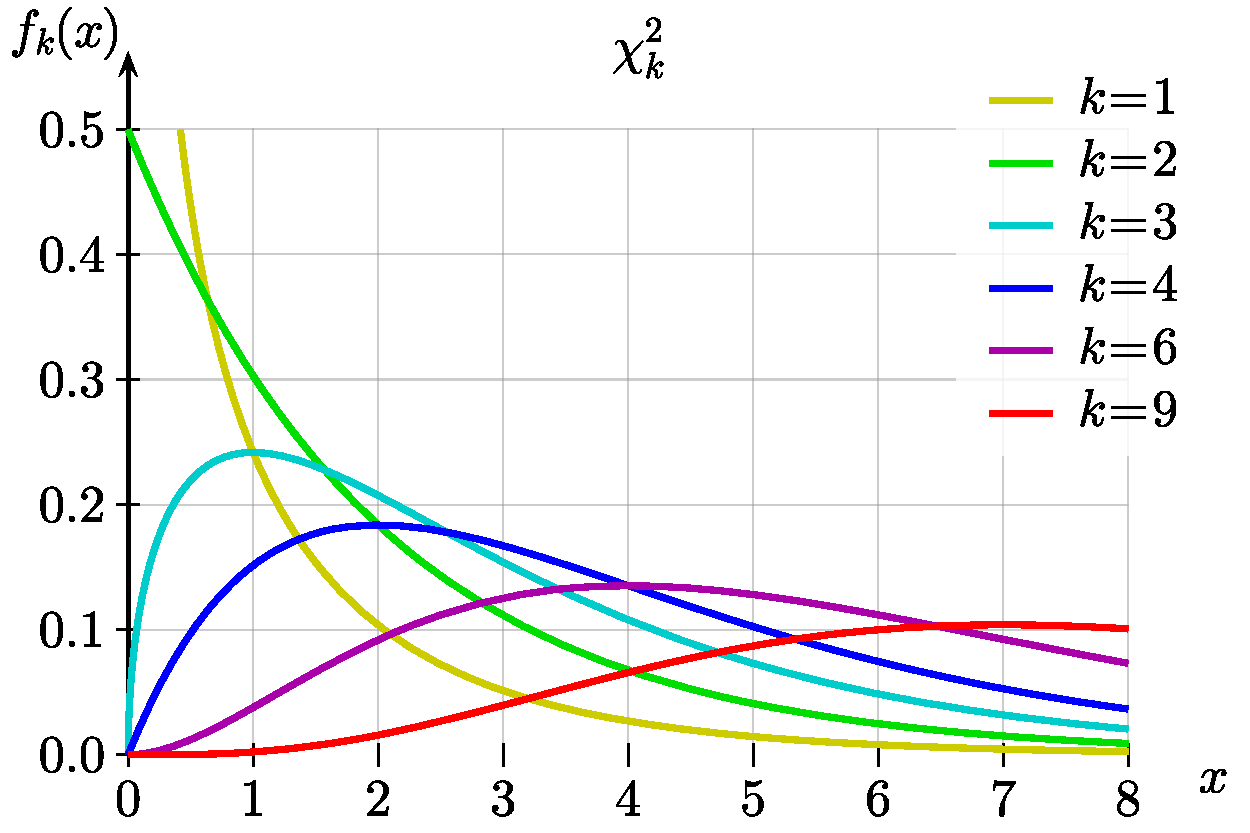
\includegraphics[width=0.7\textwidth]{figures/stats/dist/chi2_pdf}
\caption{
$\chi^{2}$-distribution PDF,
by \href{https://en.wikipedia.org/wiki/File:Chi-square_pdf.svg}{Geek3}.
Here $k$ is being used in lieu of $\nu$ for the number of degrees of freedom.
}
\label{fig:dist:chi2}
\end{figure}

\begin{figure}
\centering
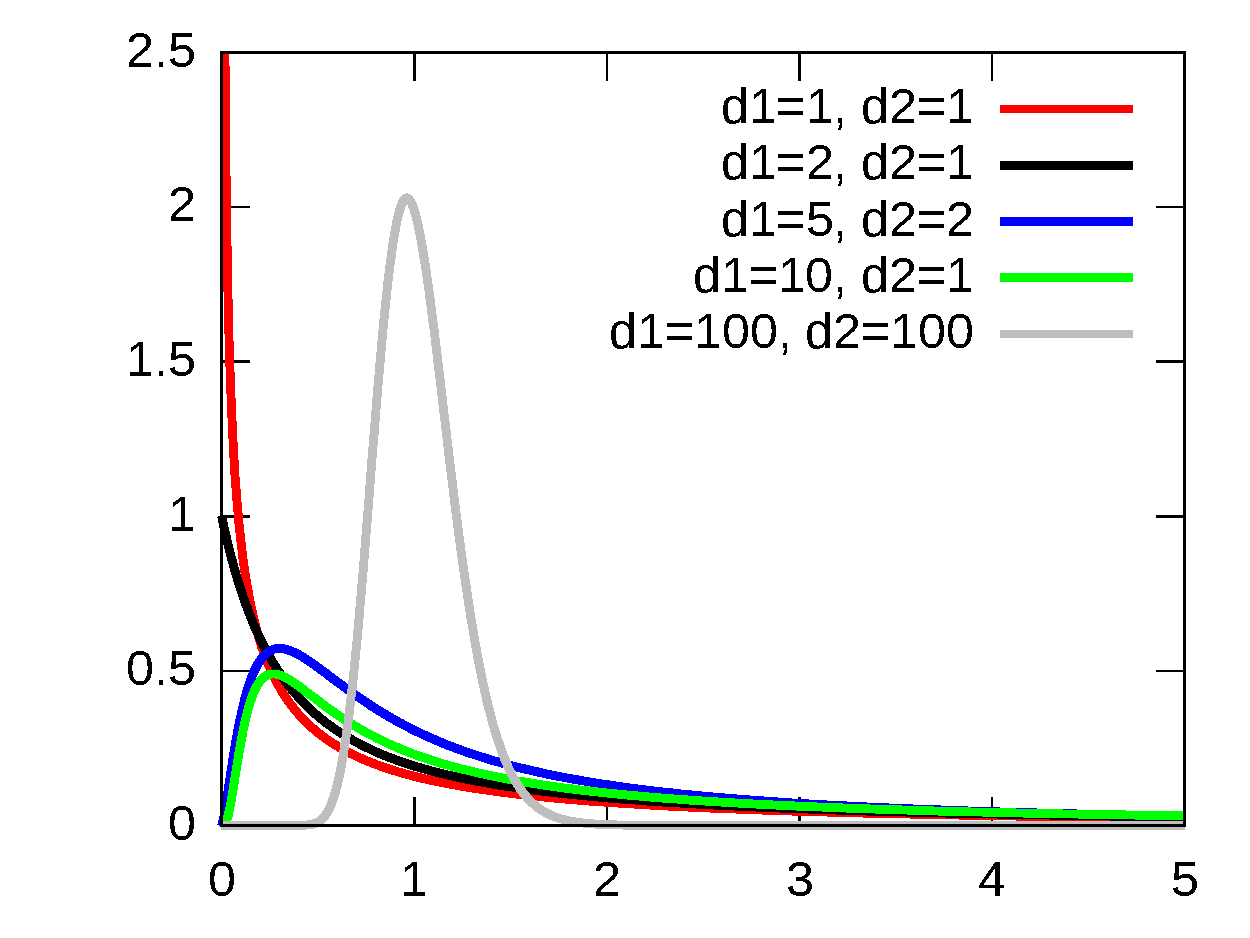
\includegraphics[width=0.7\textwidth,trim={1.5cm 0.1cm 0.1cm 0.1cm},clip]{figures/stats/dist/F_pdf}% trim={<left> <lower> <right> <upper>}
\caption{
$F$-distribution PDF,
by \href{https://en.wikipedia.org/wiki/File:F-distribution_pdf.svg}{IkamusumeFan}.
}
\label{fig:dist:F}
\end{figure}
}
%%%%%%%%%%%%%%%%%%%%%%%%%%%%%%%%%%%%%%%%%%%%%%%%%%%%%%%%%
%%%%%%%%%%%%%%%%%%%%%%%%%%%%%%%%%%%%%%%%%%%%%%%%%%%%%%%%
%%%%%%%%%%%%%%%%%%%%%%%%%%%%%%%%%%%%%%%%%%%%%%%%%%%%%%%%
\chapter{Concepts for Finance}
\label{finance}

%%%%%%%%%%%%%%%%%%%%%%%%%%%%%%%%%%%%%%%%%%%%%%%%%%%%%%%%
%%%%%%%%%%%%%%%%%%%%%%%%%%%%%%%%%%%%%%%%%%%%%%%%%%%%%%%%
\section{Stochastic Processes}
\label{finance:sp}
% TODO

%%%%%%%%%%%%%%%%%%%%%%%%%%%%%%%%%%%%%%%%%%%%%%%%%%%%%%%%
%%%%%%%%%%%%%%%%%%%%%%%%%%%%%%%%%%%%%%%%%%%%%%%%%%%%%%%%
\section{Martingale}
\label{finance:martingale}
% TODO

%%%%%%%%%%%%%%%%%%%%%%%%%%%%%%%%%%%%%%%%%%%%%%%%%%%%%%%%
%%%%%%%%%%%%%%%%%%%%%%%%%%%%%%%%%%%%%%%%%%%%%%%%%%%%%%%%
\section{Wiener Processes}
\label{finance:wiener}
% TODO

%%%%%%%%%%%%%%%%%%%%%%%%%%%%%%%%%%%%%%%%%%%%%%%%%%%%%%%%
%%%%%%%%%%%%%%%%%%%%%%%%%%%%%%%%%%%%%%%%%%%%%%%%%%%%%%%%
\section{Brownian Motion}
\label{finance:brownian}
% TODO

%%%%%%%%%%%%%%%%%%%%%%%%%%%%%%%%%%%%%%%%%%%%%%%%%%%%%%%%
%%%%%%%%%%%%%%%%%%%%%%%%%%%%%%%%%%%%%%%%%%%%%%%%%%%%%%%%
\section{Random Walks}
\label{finance:rand_walk}
% TODO

%%%%%%%%%%%%%%%%%%%%%%%%%%%%%%%%%%%%%%%%%%%%%%%%%%%%%%%%
%%%%%%%%%%%%%%%%%%%%%%%%%%%%%%%%%%%%%%%%%%%%%%%%%%%%%%%%
\section{It\^o's Lemma}
\label{finance:ito_lemma}
% TODO

%%%%%%%%%%%%%%%%%%%%%%%%%%%%%%%%%%%%%%%%%%%%%%%%%%%%%%%%
%%%%%%%%%%%%%%%%%%%%%%%%%%%%%%%%%%%%%%%%%%%%%%%%%%%%%%%%
\section{Black-Scholes Model}
\label{finance:black_scholes}
% TODO

}

%-----------------------------------------------------------------------------%
% BIBLIOGRAPHY -- Change the style to match your discipline's standards.
%-----------------------------------------------------------------------------%
\bibliographystyle{./bib/atlasBibStyleWithTitle}
\cleardoublepage
\normalbaselines %Fixes spacing of bibliography
% \addcontentsline{toc}{chapter}{Bibliography} % not needed on my system
\bibliography{./bib/bib}
%-----------------------------------------------------------------------------%

%-----------------------------------------------------------------------------
\end{document}
